%%%%%%%%%%%%%%%%%%%%%%%%%%%%%%%%%%%%%%%%%%%%%%%%%%%%%%%%%%%%%%%
%
% Welcome to Overleaf --- just edit your LaTeX on the left,
% and we'll compile it for you on the right. If you open the
% 'Share' menu, you can invite other users to edit at the same
% time. See www.overleaf.com/learn for more info. Enjoy!
%
%%%%%%%%%%%%%%%%%%%%%%%%%%%%%%%%%%%%%%%%%%%%%%%%%%%%%%%%%%%%%%%
\documentclass[12pt,a4paper,oneside]{book}


\usepackage[T1]{fontenc}
\usepackage[utf8]{inputenc}
\usepackage{arabtex}
\usepackage{utf8}
\setcode{utf8}
\usepackage{setspace}
\usepackage[T1]{fontenc}
\usepackage[french]{babel}
\usepackage{svg}
\usepackage{amsmath}
\usepackage{amsthm}
\usepackage{amssymb}
\usepackage{tikz}
\usepackage{tcolorbox}
\usepackage{tabularx}
\usetikzlibrary{calc}
\usepackage[french,ruled,vlined]{algorithm2e}
\usepackage{rotating}
\usepackage{bbding}
\usepackage{cite}
\usepackage{lscape,graphicx}
\usepackage{rotating}
\usepackage{setspace}
\usepackage{sectsty}
\usepackage{dsfont}
\usepackage{ifpdf}
\usepackage{subfigure}
\usepackage{epsfig}
\usepackage{float}
\usepackage{titlesec}
\usepackage{multibib}
\usepackage{fancyhdr}
\usepackage{lipsum}
\usepackage{soul}
\usepackage{fancyhdr}

\usepackage[paperwidth=210mm,paperheight=297mm,tmargin=15mm,lmargin=20mm]{geometry}
%
\renewcommand{\topfraction}{0.9}
\renewcommand{\textfraction}{0.1}
\renewcommand{\floatpagefraction}{0.8}
%

\usepackage{hyperref}

\hypersetup{
    colorlinks=true,
    linkcolor=blue,     % Couleur des liens internes
    citecolor=blue,     % Couleur des citations
    filecolor=magenta,  % Couleur des liens vers des fichiers
    urlcolor=cyan       % Couleur des liens externes
}
\urlstyle{same}

\setlength{\headheight}{30pt}

\pagestyle{fancy}% \renewcommand{\chaptermark}[1]{\markboth{#1}{}}
\renewcommand{\chaptermark}[1]{\markboth{\MakeUppercase{#1}}{}}
\renewcommand{\sectionmark}[1]{\markright{{\thesection.\ #1}}}


%
% \renewcommand{\sectionmark}[1]{\markright{#1}}
%\renewcommand \thesection{\Roman{section}.}
%\renewcommand \thesubsection{\alph{subsection}.}
%
%\newcommand{\helv}{%
%\fontfamily\fontsize{9}{11}\selectfont}

%

% Clear Header Style on the Last Empty Odd pages
\makeatletter
  \def\cleardoublepage{\clearpage\if@twoside \ifodd\c@page\else%
      \hbox{}%
       \thispagestyle{empty}%              % Empty header styles
       \newpage%
       \if@twocolumn\hbox{}\newpage\fi\fi\fi}
\makeatother


% \fancyhead[RE]{\textit{\nouppercase{\leftmark}}}
% \fancyhead[LO]{\textit{\nouppercase{\rightmark}}}
% \fancyhead[LE,RO]{\thepage}

% \renewcommand{\headrulewidth}{0pt}
% \renewcommand{\footrulewidth}{0pt}
%
\setcounter{secnumdepth}{4}
\setcounter{tocdepth}{4}
%

%
\def\ds{\displaystyle}
\def\dir{./figures}

%


%\setlength\topmargin{0in}
%\setlength\topmargin{0in}
%

%
% Remove page numbering from first page Bibliography
%
%%%%%%%%%%%%%%%%%%%%%%%%% Page de titre %%%%%%%%%%%%%%%%%%%%%%%
\def\baselinestretch{1.5}


\usepackage{listings}
\usepackage{caption}
\usepackage{longtable}

\usepackage{geometry}
\usepackage{booktabs}

\geometry{
    letterpaper,
    left=1.5cm,
    right=1.5cm,
    top=1.5cm,
    bottom=1.5cm
}

\usepackage{afterpage}

\newcommand\blankpage{%
    \null
    \thispagestyle{empty}%
    \addtocounter{page}{-1}%
    \newpage}


\usepackage[acronym]{glossaries}

\usepackage{lmodern}


\newenvironment{dedication}
  {%\clearpage           % we want a new page          %% I commented this
   \thispagestyle{empty}% no header and footer
   \vspace*{\stretch{1}}% some space at the top
   \itshape             % the text is in italics
   \raggedleft          % flush to the right margin
  }
  {\par % end the paragraph
   \vspace{\stretch{3}} % space at bottom is three times that at the top
   \clearpage           % finish off the page
  }




  \fancyheadoffset{0pt} % Pas de décalage par rapport à la marge gauche

% En-têtes



%\makenoidxglossaries 

%\newglossaryentry{latex}
%{
       % name=latex,
        %description={Is a mark up language specially suited for scientific documents}
%}



%\selectlanguage{English}



\hypersetup{
    colorlinks=true,
    linkcolor=black,
    filecolor=magenta,      
    urlcolor=cyan,
    pdfauthor={Name},  %put your name here
    pdftitle={PDF_TTILE},  %PDF title
    pdfpagemode=FullScreen,
    }



\begin{document}



\definecolor{codegreen}{rgb}{0,0.6,0}
    \definecolor{codegray}{rgb}{0.5,0.5,0.5}
    \definecolor{codepurple}{rgb}{0.58,0,0.82}
    \definecolor{backcolour}{rgb}{0.95,0.95,0.92}
    
    \lstdefinestyle{mystyle}{
        backgroundcolor=\color{backcolour},   
        keywordstyle=\color{magenta},
        numberstyle=\tiny\color{codegreen},
        stringstyle=\color{codepurple},
        basicstyle=\ttfamily\footnotesize,
        breakatwhitespace=false,         
        breaklines=true,                 
        captionpos=b,                    
        keepspaces=true,                 
        numbers=left,                    
        numbersep=5pt,                  
        showspaces=false,                
        showstringspaces=false,
        showtabs=false,                  
        tabsize=2
    }




%
\thispagestyle{empty}

\includegraphics[scale=0.08]{Logos/Logo_INPT.png} 
         \hspace{11cm}  

\includegraphics[scale=0.1]{Logos/Logo_ANRT.jpg}
        
\vspace{0.9cm}
\begin{center}
{\large \textsc{\textbf{Mémoire du projet de fin d'études}}}\\[0.1cm]
{\large \textsc{Pour L'obtention du Diplôme d'Ingénieur d'État}}\\[0.1cm]
{\large \textsc{\textit{Filière: XXXXXXXXXXXX}}} \\[0.05cm] 
\vspace{-0.04cm}
% Title
\rule{\linewidth}{0.3mm} \\[0.4cm]   % à ajuster l'éspace en cas de besoin: [1cm]
 { \huge \textbf{ Titre de Projet }} \\[0.15cm] 
\rule{\linewidth}{0.3mm} \\[0.4cm]
\vspace{0.4cm}


\includegraphics[scale=0.075]{Logos/Company_Logo_Expl.png}  %change the scale to suit your logo

\vspace{1cm}

% Author and supervisor
\noindent
\begin{minipage}{0.9\textwidth}
    \vspace{-7mm}
  \begin{flushleft} \large
    \emph{Réalisé par :}\\
    Mme / M. Xxxx \textsc{XXXX} %\& Mme / M. Xxxx \textsc{XXXX}  %Au cas de binôme, remove the % \\
  \end{flushleft}
\end{minipage}
\begin{minipage}{0.4\textwidth}

\end{minipage}\\[0.6cm]

{\large \textit{Soutenu le XX Juillet 20XX, devant le jury composé de : }}\\[0.5cm]


\begin{tabular}{p{1cm}lll}
 & \large M / Mme. Xxxx \textsc{XXXX}  & \large INPT & \large - Examinateur/trice \\[0.1cm]
 & \large M / Mme. Xxxx \textsc{XXXX}  & \large INPT & \large - Examinateur/trice \\[0.1cm]
 & \large M / Mme. Xxxx \textsc{XXXX}  & \large INPT & \large - Encadrant/e \\[0.1cm]
  & \large M / Mme. Xxxx \textsc{XXXX}  & \large Entreprise & \large - Encadrant/e \\[0.1cm]
 
\end{tabular}

\vspace{0.5cm}

\includegraphics[scale=0.6]{Logos/ZLAFA.png}


\textsc{Agence National de Réglementation des Télécommunications}\\
\textsc{Institut National des Postes et Télécommunications}
% Bottom of the page

%\vspace{0.3cm}
{\large Promotion : 20XX/20XX}
   
\end{center}


 %FRENCH ONE


\thispagestyle{empty}

\includegraphics[scale=0.08]{Logos/Logo_INPT.png} 
         \hspace{12cm}  
         
\includegraphics[scale=0.35]{Logos/Logo-4D.jpg}
        
\vspace{0.5cm}
\begin{center}
{\large \textsc{\textbf{Mémoire du projet de fin d'études}}}\\[0.1cm]
{\large {Pour l’obtention du Diplôme d’Ingénieur d’État en Télécommunications 
et Technologies de l’Information.}}\\[0.1cm]
{\large \textsc{\textit{Filière:\textbf{ Advanced Software Engineering for Digital Services (A.S.E.D.S)}}}} \\[0.05cm] 
\vspace{0.5cm}
\vspace{-0.04cm}
% Title
\rule{\linewidth}{0.3mm} \\[0.4cm]   % à ajuster l'éspace en cas de besoin: [1cm]
 { \huge \textbf{ Développement d’une plateforme de formation en ligne pour 4D }} \\[0.15cm] 
\rule{\linewidth}{0.3mm} \\[0.4cm]


  %change the scale to suit your logo

\vspace{1cm}

% Author and supervisor
\noindent
\begin{minipage}{0.9\textwidth}
    \vspace{-7mm}
  \begin{flushleft} \large
    \emph{Réalisé par :}\\
    Mme. \textsc{HSAINI} Abir %\& Mr/Mrs/Ms. Xxxx \textsc{XXXX}  %Au cas de binôme, remove the % \\
  \end{flushleft}
\end{minipage}
\begin{minipage}{0.4\textwidth}

\end{minipage}\\[0.4cm]

{\large \textit{Soutenu le 24 Juin 2024, devant les membres de jury : }}\\[0.3cm]


\begin{tabular}{p{1cm}lll}
  & \large Pr. HAFIDDI Hatim & \large INPT & \large - Encadrant interne \\[0.1cm]
  & \large Pr. CHAMI Mouhcine & \large INPT & \large - Examinateur  \\[0.1cm]
  & \large Pr. LAGHOUAOUTA Youness & \large INPT & \large - Examinateur \\[0.1cm]
  & \large M. METWALLI Ayoub & \large 4D & \large - Encadrant externe  \\[0.1cm]
\end{tabular}


\includegraphics[scale=0.65]{Logos/ZLAFA.png}


\textsc{Agence National de Réglementation des Télécommunications}\\
\textsc{Institut National des Postes et Télécommunications}
% Bottom of the page

%\vspace{0.3cm}
{\large Année universitaire : 2023/2024}
   
\end{center}


 % ENGLISH

\afterpage{\blankpage}  %page vide obligatoire

\frontmatter


\chapter*{Dédicace}
\addcontentsline{toc}{chapter}{Dédicaces}
% \begin{center}
%     \emph{To my family, who supported me\\
%     throughout this journey.}
% \end{center}


% Define custom colors
\definecolor{dedicationquote}{RGB}{0, 0, 0}
\definecolor{signature}{RGB}{153, 153, 153}

% Define custom commands for dedication quote and signature
\newcommand{\dedicationquote}[1]{%
    \begin{quote}
    \begin{center}
        \large\itshape\color{dedicationquote}
        #1
    \end{center}
    \end{quote}
}

% \newcommand{\dedicationquote}[1]{
%     \begin{quote}
%         \large\itshape\color{dedicationquote}
%         #1
%     \end{quote}
% }

\newcommand{\signature}[1]{%
    \begin{flushright}
        \color{signature}
        \emph{#1}
    \end{flushright}
}
\vspace{1cm}
\hspace{0.4cm}

\includegraphics[scale=0.02]{Logos/quote2.png}
\hspace{5cm}
    
\dedicationquote{ À Dieu tout puissant mon créateur:\\[0.3cm]
À mes chers parents, Quoi que je fasse ou que je dise, je ne pourrai pas vous remercier comme il se doit. Votre affection me couvre, votre bienveillance me guide et votre présence à mes côtés a été toujours une source de force pour affronter les différents obstacles.\\[0.3cm]
À mon frère Mohammed Amine, qui était comme un père pour moi, et aussi un endroit de sécurité et de soutien. Ce travail est le fruit de ton abnégation tout au long de mes années d’études.\\[0.3cm]
À toute ma famille et mes amis, qui m’ont toujours motivé et à qui je souhaite un succès encore plus grand.\\[0.3cm]
Et à tous ceux qui ont cru en moi,\\[0.3cm]
Je dédie ce travail…\\
}


\hspace{15cm}

\includegraphics[scale=0.02]{Logos/quote1.png}
\vspace{1cm}
\signature{- Abir}




\chapter*{Remerciements}
\addcontentsline{toc}{chapter}{Remerciements}


Tout d’abord, je remercie Allah le tout-puissant de m’avoir donné le courage et la patience nécessaires à mener ce travail à son terme.

\vspace{10pt}
Je tiens à remercier toutes les personnes qui par leur support ou par leur simple présence, m'ont permis de rendre mon travail aussi instructif et bénéfique que plaisant.

\vspace{10pt}
Je transmets mes sincères remerciements à mon encadrant \textbf{M. HAFIDDI \textsc{Hatim}} qui m'a allégé par ses connaissances, son savoir et ses précieuses orientations, pour les conseils qu’il a prodigués, et le suivi pertinent, mais aussi pour la fierté et l’ambition que j'ai acquises suite à l’encouragement et le support intensif, ainsi que l’assistance précieuse.

\vspace{10pt}
Je tiens également à remercier, chaleureusement, mon encadrant externe, \textbf{M. METWALLI \textsc{Ayoub}} pour sa confiance, sa collaboration et son soutien, et de m’avoir supervisé tout au long de mon stage par ses conseils, ses orientations et son sens de rigueur qui m’a guidé durant ce travail et de m’avoir permis de m’intégrer. Je tiens aussi à témoigner toute ma reconnaissance aux membres de l’entreprise 4D, pour l’expérience enrichissante et pleine d’intérêt qu’ils m’ont fait vivre durant ces mois de stage parmi eux.

\vspace{10pt}
Je tiens à remercier également les membres de jury, \textbf{M. LAGHOUAOUTA \textsc{Youness}} et Monsieur \textbf{M. CHAMI \textsc{Mouhcine}}, pour l’évaluation du travail réalisé. Mes remerciements s’adressent aussi à l’ensemble du corps enseignant de l’institut national des postes et télécommunications (INPT), pour le temps qu’ils ont consacré pour nous offrir une formation d’excellence et de polyvalence et à toutes les personnes qui nous ont été d’une aide précieuse.



\chapter*{Résumé}
\addcontentsline{toc}{chapter}{Résumé}


\hspace{10pt}Le présent document constitue une synthèse du travail réalisé dans le cadre de mon projet de fin d’études au sein de la société 4D Logiciels pour l’obtention du diplôme d’ingénieur d’état en développement des services numériques.

\vspace{10pt}

J'ai été chargé par l'entreprise de développer une plateforme de formation en ligne pour 4D. Ce projet interne de l'entreprise vise à fournir aux employées de la société ainsi que les clients un espace partagé où ils peuvent consulter les différentes formations, qu’elles portent sur 4D ou d’autres sujets.

\vspace{10pt}

Pour réussir ce projet, nous avons commencé par une analyse approfondie du projet dans le but d’identifier les besoins fonctionnels et techniques, auxquels la solution doit répondre. Dans une seconde étape, nous avons mené une étude conceptuelle traduite en diagrammes. Finalement, nous avons initié le développement et la mise en œuvre de la solution.

\vspace{10pt}

Le projet a été mis en œuvre en utilisant le Framework React coté Front End et 4D pour le backend.

\vspace{10pt}


\noindent\rule[2pt]{\textwidth}{0.5pt}

{\textbf{Mots clés :}}
React , typescript , 4D, E-learning 
\\
\noindent\rule[2pt]{\textwidth}{0.5pt}

% \cleardoublepage
%

\chapter*{Abstract}
\addcontentsline{toc}{chapter}{Abstract}

Nowadays, the demand for digital transformation is continuously increasing, especially after the COVID-19 pandemic. In this context, digital platforms play a crucial role in digitizing various sectors and creating value.

\vspace{10pt}


This work is part of my end-of-studies project carried out within the company 4D in order to obtain the title of State Engineer in Digital Services Development at the National Institute of Posts and Telecommunications.

\vspace{10pt}

My mission was to develop an online training platform for 4D. This internal project of the company aims to provide employees of the company as well as clients with a shared space where they can access various training sessions, whether they are related to 4D or other subjects.

\vspace{10pt}

To succeed in this project, we started with a thorough analysis of the project in order to identify the functional and technical requirements that the solution must meet. In a second step, we conducted a conceptual study translated into diagrams. Finally, we initiated the development and the implementation of the solution.

\vspace{10pt}

The project was implemented using React framework for frontend and 4D for backend.

\vspace{10pt}

\noindent\rule[2pt]{\textwidth}{0.5pt}

{\textbf{Key Words :}}
React, TypeScript, 4D, E-learning, Tailwind, Frontend, Backend 
\\
\noindent\rule[2pt]{\textwidth}{0.5pt}

% \cleardoublepage
%

\chapter*{\RL{ملخص}}
\addcontentsline{toc}{chapter}{Arabic Abstract}

\begin{RLtext}

 \noindent ملخص بالعربية، تأكد من أن الترجمة منطقية


\end{RLtext}

\noindent\rule[2pt]{\textwidth}{0.5pt}

\begin{RLtext} 

{\textbf{الكلمات المفتاحية}}

مثال
\\

\end{RLtext}

\noindent\rule[2pt]{\textwidth}{0.5pt}

% \cleardoublepage
%






\listoffigures
\addcontentsline{toc}{chapter}{Table des figures} 
%figures are added automatically here

\listoftables
\addcontentsline{toc}{chapter}{Liste des tableaux} 
%tables are added automatically here

\lstlistoflistings
\addcontentsline{toc}{chapter}{Listings} 
%Code snippets are added automatically here


\tableofcontents
\addcontentsline{toc}{chapter}{Table des matières}
%contents are added automatically here



\mainmatter

\chapter*{Introduction générale}
\addcontentsline{toc}{chapter}{Introdcution}


Dans un monde avec une grande évolution, où les technologies changent rapidement, la nécessité d'une formation continue efficace, simple et accessible est devenue primordiale pour rester présent sur le marché du travail. Les entreprises et les individus reconnaissent de plus en plus l’importance d'une formation continue en certains domaines pour améliorer leurs compétences, acquérir de nouvelles connaissances et s'adapter aux changements rapides de l'environnement professionnel.\\

C'est dans ce contexte que s'inscrit notre projet de fin d'études (PFE), qui vise à créer une plateforme de formation continue adaptée aux besoins actuels des employés et des clients de 4D. L’objectif principal de notre projet est de fournir une solution technologique robuste et conviviale qui facilite l'accès aux différentes formations du langage 4D ainsi que les autres langages, tout en offrant des fonctionnalités avancées pour suivre, évaluer et personnaliser le processus d'apprentissage.\\

Ce rapport présente le processus de développement de notre plateforme de formation continue, composé de quatre chapitres. Dans le premier chapitre, nous exposons le contexte général du projet, à savoir, la présentation de l’organisme d’accueil 4D Logiciels, le contexte général et la conduite du projet. Le deuxième chapitre est dédié à l’analyse et à la spécification des besoins pour développer cette plateforme. Le troisième chapitre porte sur la définition des architectures utilisées, ainsi que la modélisation des diagrammes de classes et de séquence. Enfin, dans le quatrième chapitre, nous abordons l’implémentation et la validation de la solution, suivies par une conclusion générale où nous discutons des perspectives d’évolution.\\


%debut of chapters

\chapter{Contexte général du projet}
\label{chap:Contexte général du projet}



Dans ce chapitre, nous situons notre stage de fin d’études dans son environnement organisationnel et contextuel. Nous présentons l’organisme d’accueil 4D logiciel. Ensuite nous expliquons la méthodologie adoptée durant la réalisation de notre projet ainsi que sa planification.

\newpage


\section{Pésentation de l’organisme d’accueil}

\begin{figure}[h]
    \centering
    
\includegraphics[scale=0.5]{Logos/Logo-4D.jpg} % Replace with the actual filename of the IBM logo image
    \caption{Logo 4D }
    \label{fig:Logo4D}
\end{figure}

Fondée en 1984 par Laurent Ribardière, 4D Logiciels est une entreprise de conseil et de développement de logiciels dans le domaine des systèmes d’information, de l’organisation et de l’informatique, dont le siège social se situe à Clichy (Île-de-France). Ribardière a créé 4D avec une seule ambition : simplifier la création des applications professionnelles pour les entreprises grâce à une base de données relationnelles entièrement graphique. 4D est ainsi devenue l’un des premiers éditeurs de logiciels français avec un rayonnement international, grâce à sa présence sur les cinq continents et des filiales dans plus de dix pays, dont le Maroc (4D Logiciels Maroc). Son succès vient de sa capacité à répondre aux enjeux de son époque grâce à une plateforme évolutive, facilitant la création d’expériences clients réussies sur mobile, web et desktop. \cite{ref1}

%%%%%%%%%%%%%%%%%%%% subsection 1 %%%%%%%%%%%%%%%%%%%%%%%

\subsection{Histoire de 4D}


\begin{figure}[h]
    \centering
    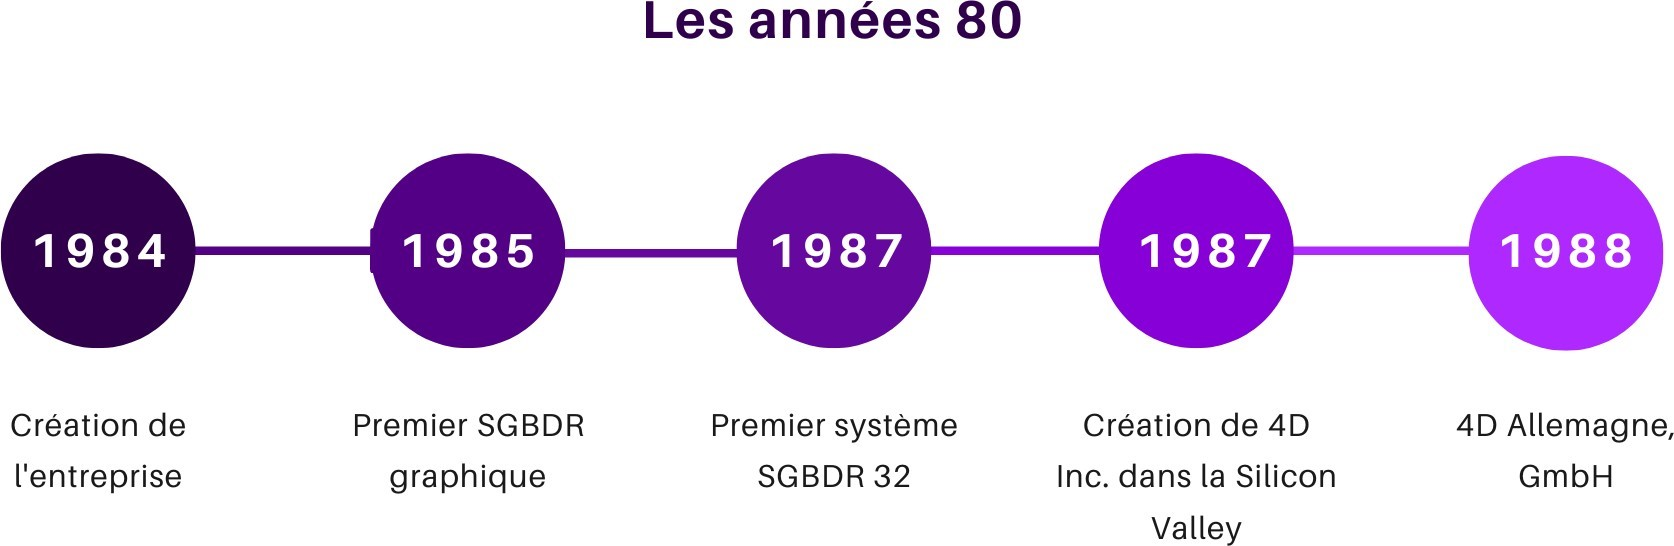
\includegraphics[scale=0.3]{Figures/80.jpg} % Replace with the actual filename of the IBM logo image
    \caption{Les années 80 \cite{4Dhistory}}
    \label{fig:Histoire80}
\end{figure}


En 1987 , 4D Logiciels propose le premier système de gestion de base de données relationnel fonctionnant sur un système 32-bits, puis conserve sa place de leader en offrant le premier :
\begin{itemize}
    \item[$\bullet$]  Client-serveur intégré.
    \item[$\bullet$]  Serveur web intégré.
    \item[$\bullet$]  Système de partage d’applications dynamique intégré.
\end{itemize}
\vspace{1cm}

\begin{figure}[h]
    \centering
    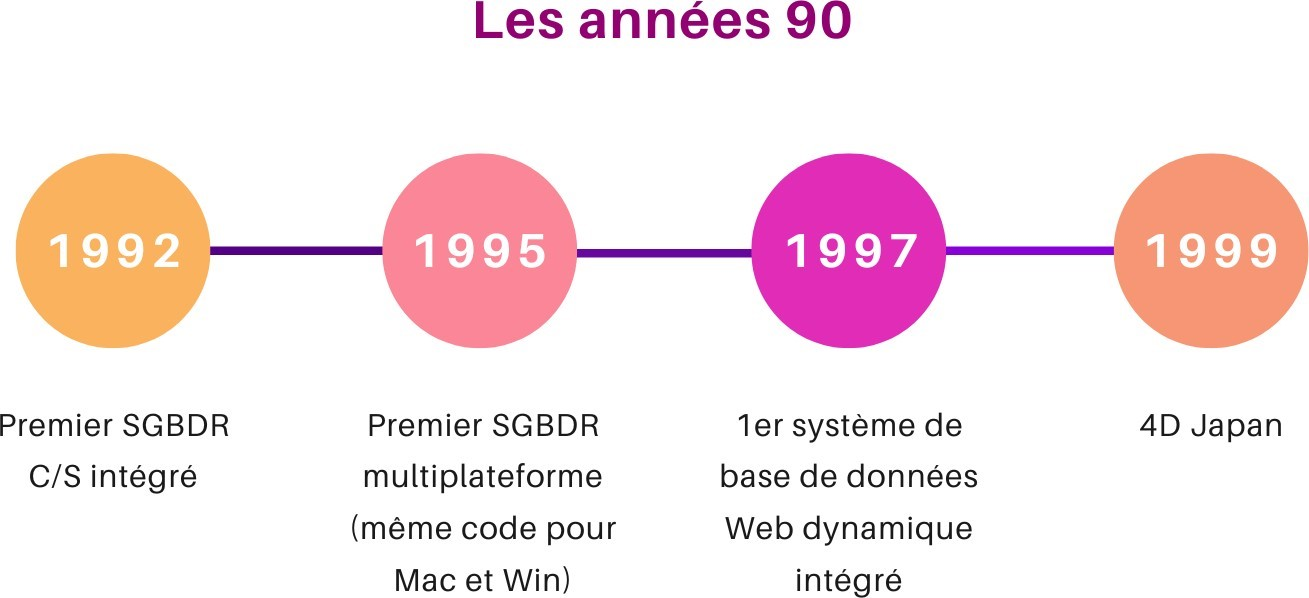
\includegraphics[scale=0.3]{Figures/90.jpg} % Replace with the actual filename of the IBM logo image
    \caption{Les années 90 \cite{4Dhistory}}
    \label{fig:Histoire90}
\end{figure}
% \vspace{lcm}

En 1997, 4D décide de s’investir dans le Web en donnant lieu 
à un serveur Web dynamique. Ce qui aide les développeurs à servir
à la fois des applications client-serveur et des applications
Web sans modifier le code. 4D conserve par la suite ce produit 
en lançant à chaque fois des nouvelles versions.

\begin{figure}[h]
    \centering
    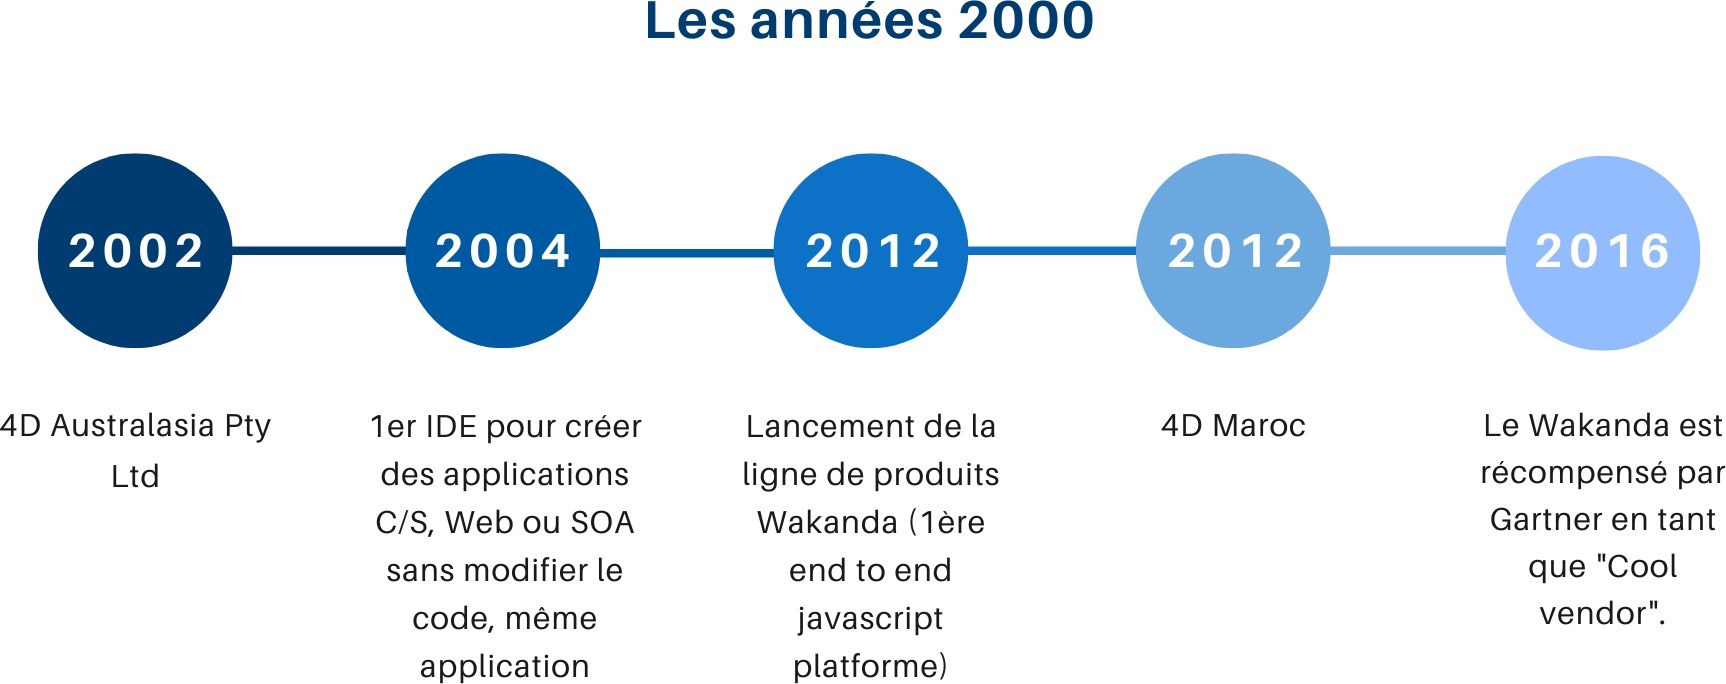
\includegraphics[scale=0.3]{Figures/20.jpg} % Replace with the actual filename of the IBM logo image
    \caption{Les années 2000 \cite{4Dhistory}}
    \label{fig:Histoire90}
\end{figure}

La version 4D 2004 se lance en tant qu’un produit permettant aux développeurs 
de créer à la fois des applications autonomes, client-serveur, Web, 
ainsi que des applications orientées Services (SOA) sans rajouter 
aucun changement au niveau du code.
Plus récemment, 4D dispose d’une plateforme de développement 
en JavaScript qui facilite la création des applications 
professionnelles en utilisant la gamme de produits Wakanda.


%%%%%%%%%%%%%%%%%%%% subsection 2 %%%%%%%%%%%%%%%%%%%%%%%

%%%%%%%%%%%%%%%%%%%% subsection 3 %%%%%%%%%%%%%%%%%%%%%%%

\subsection{La structure du groupe 4D}

Le groupe 4D est composé d’un siège social situé en France, 
et de cinq filiales situées aux États-Unis, en Allemagne, 
en Australie, au Japon, et au Maroc. À l’écoute permanent 
de leurs besoins et des évolutions technologiques, 
la société offre une expérience enrichissante dans un contexte multiculturel grâce à ses différentes implantations internationales (Sydney, Tokyo, San José, Munich, Rabat).

\vspace{1cm}

\begin{figure}[h]
    \centering
    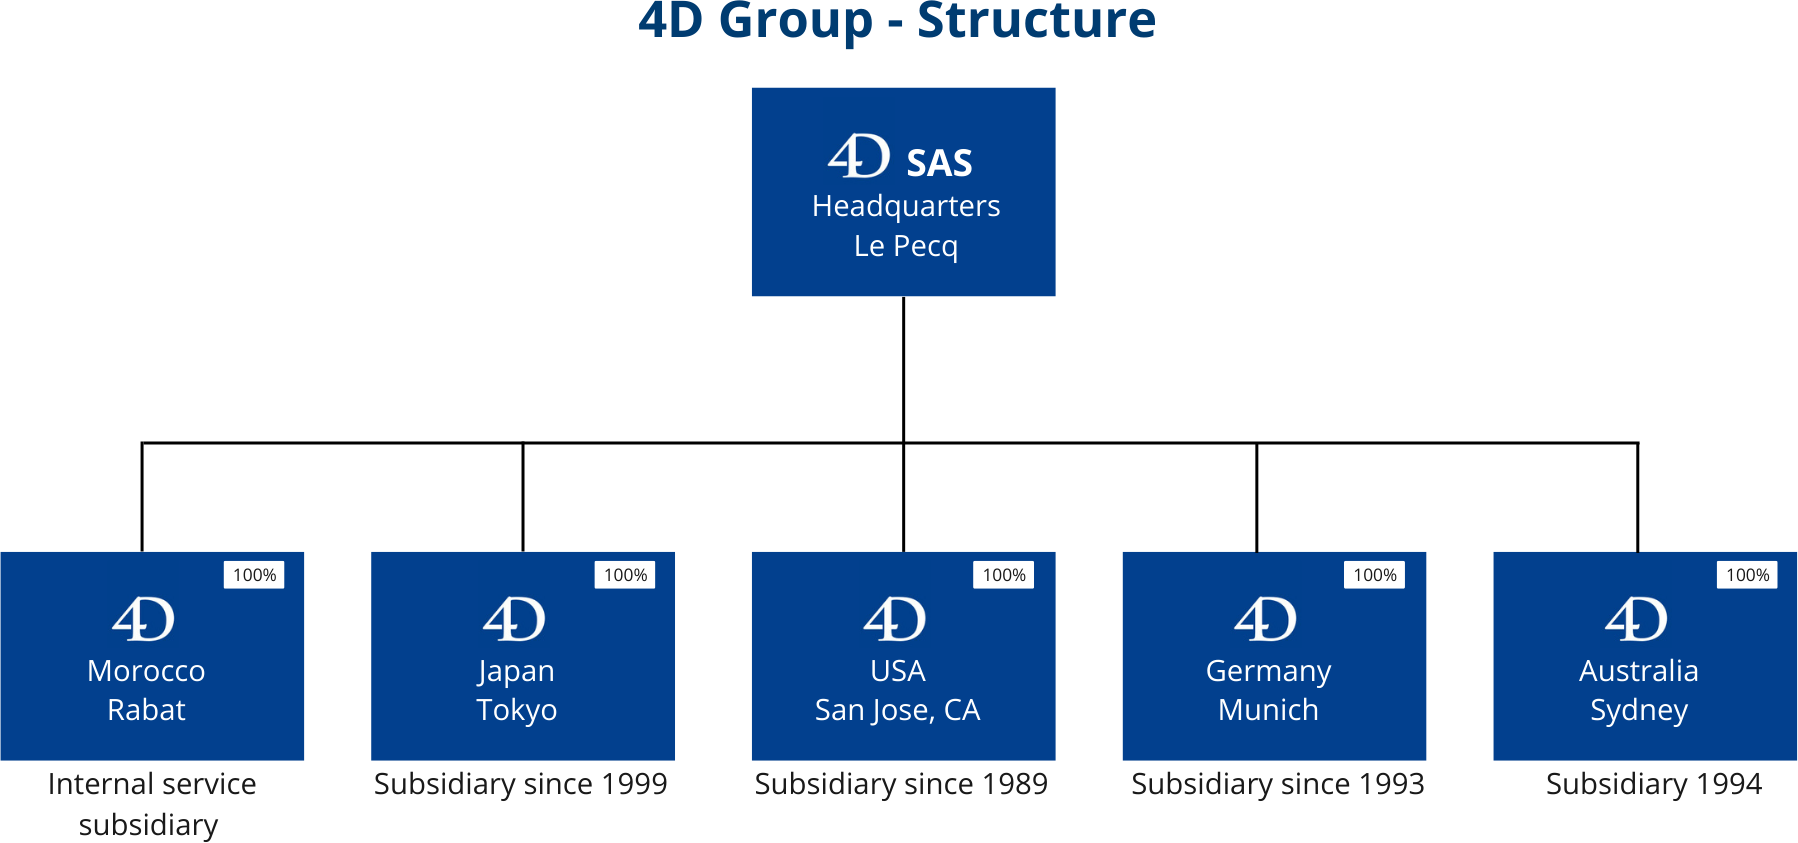
\includegraphics[scale=0.35]{Figures/groupe.png} % Replace with the actual filename of the IBM logo image
    \caption{Le groupe 4D dans le monde}
    \label{fig:groupe}
\end{figure}

Comme toute société renommée, 4D recourt à ses différents partenaires 
pour un rendu meilleur et un niveau d’expertise plus crédible. 4D connaît aussi 
une présence internationale grâce à ses partenaires et ses distributeurs éparpillés 
dans le monde, comme montre la figure suivante :

\begin{figure}[h]
    \centering
    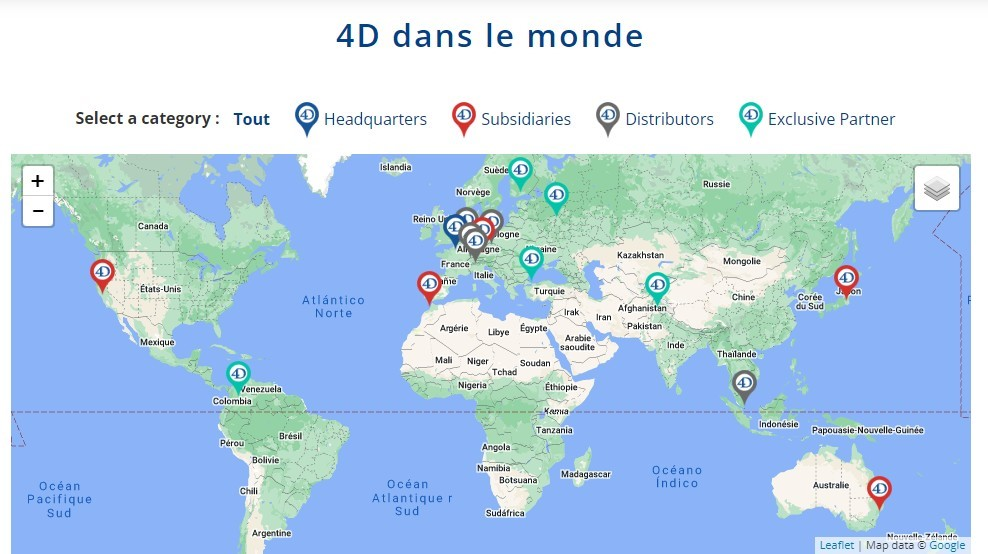
\includegraphics[scale=0.6]{Figures/carte.jpg} % Replace with the actual filename of the IBM logo image
    \caption{Les points de présence des partenaires et des distributeurs de 4D \cite{4Dhistory}}
    \label{fig:carte}
\end{figure}

\vspace{6cm}

La figure ci-dessous montre la direction générale de l’entreprise 4D logiciels :



\begin{figure}[h]
    \centering
    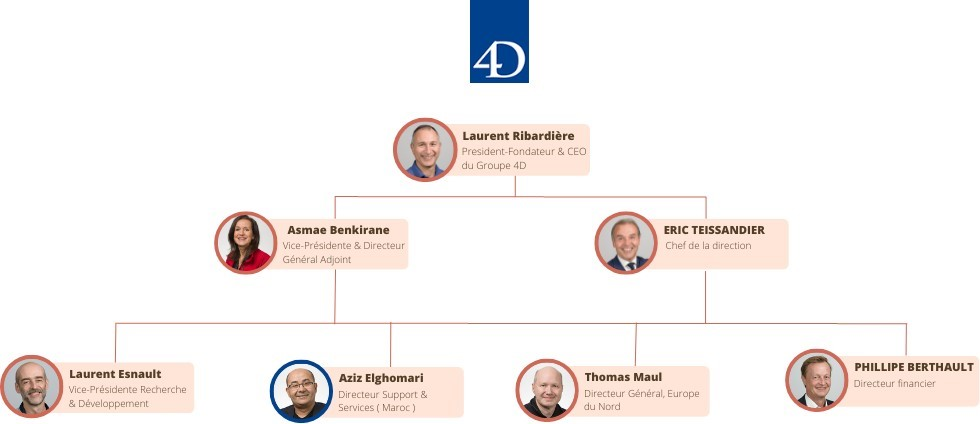
\includegraphics[scale=0.6]{Figures/direction.jpg} % Replace with the actual filename of the IBM logo image
    \caption{La Direction Générale de 4D}
    \label{fig:direction}
\end{figure}

%%%%%%%%%%%%%%%%%%%% subsection 4 %%%%%%%%%%%%%%%%%%%%%%%
\subsection{Les domaines métiers et les clients 4D}
4D intervient dans une diversité de domaines, comme 
la santé, l’éducation, l’administration, la gouvernance, 
et les télécommunications. La figure 1.8 montre le pourcentage 
qu’occupe chaque domaine dans son activité.

\begin{figure}[h]
    \centering
    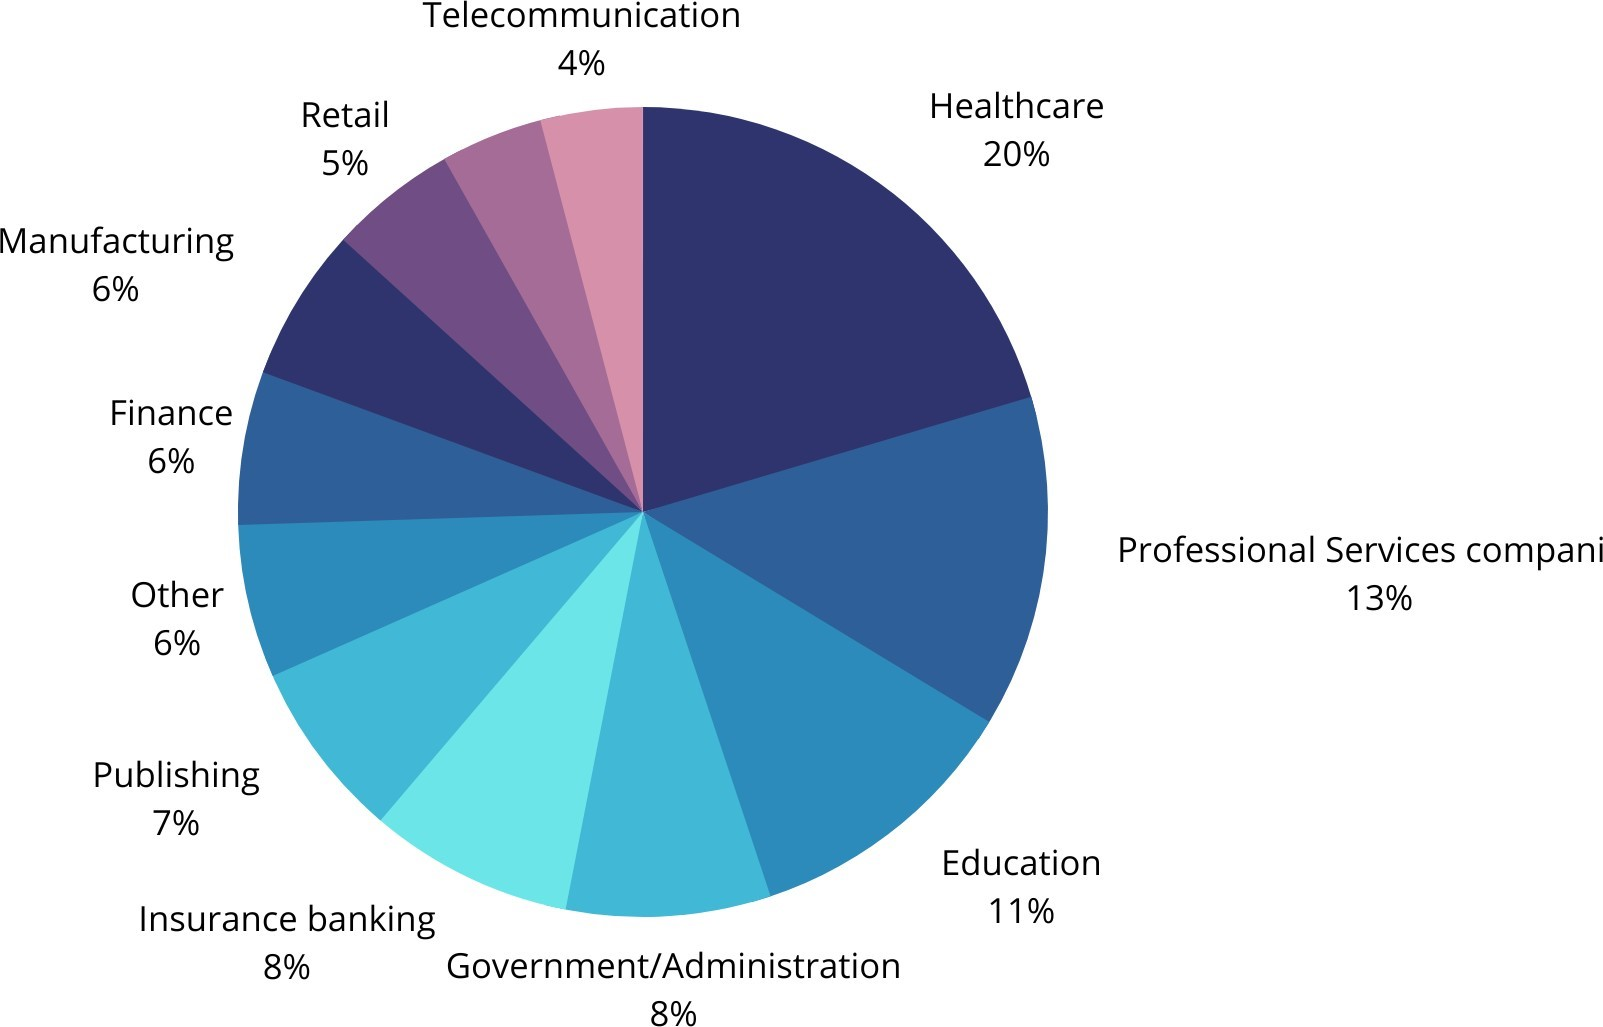
\includegraphics[scale=0.7]{Figures/domaineMetier.jpg} % Replace with the actual filename of the IBM logo image
    \caption{Les domaines métiers de 4D en pourcentage}
    \label{fig:domaineMetier}
\end{figure}


%%%%%%%%%%%%%%%%%%%% SECTION 3 %%%%%%%%%%%%%%%%%%%%%%%


\subsection{Le Langage 4D}

4D est une plateforme de développement productive qui permet aux clients
 de se concentrer sur leur modèle de données et les règles 
 et spécificités de leur métier \cite{ref1}.

 4D Serveur exécute leurs applications simultanément sur les postes de travail
/ clients mobiles et sur le Web. Ils peuvent déployer des applications 
entièrement personnalisées sous leur propre marque.
 4D est un système de gestion de base de données 
 relationnelle disposant d’un langage de programmation 
 de la quatrième génération.

Environnement de développement intégré, 4D intègre :
\begin{itemize}
    \item un compilateur;
    \item un débogueur;
    \item un système de sauvegarde et de réplication;
    \item un serveur Web;
    \item un serveur et client de services web.
\end{itemize}


4D v18 marque un véritable tournant dans l’histoire de 4D. Cette version propose non seulement de
multiples nouvelles fonctionnalités, mais aussi l’amélioration de fonctions existantes. Elle introduit la gestion de version pour changer 
la façon dont les équipes collaborent. Le format texte des bases projets permet désormais de tirer pleinement parti des systèmes de gestion de version
(par exemple, Git, SVN, etc.). Autre fonctionnalité qui fait ses débuts dans cette nouvelle version : une solution intégrée de chiffrement des données, 
offrant en un seul clic une sécurité maximum aux données des clients. Ces outils de chiffrement sont basés sur l’un des algorithmes les plus sûrs : 
Advanced Encryption Standard (AES). ORDA (Object Relational Data Access), la technologie révolutionnaire d’accès et de présentation 
des données, apporte également son lot de nouvelles fonctionnalités, telles que le Datastore distant, ouvrant de nouvelles perspectives et optimisant les 
performances du client/serveur. Les applications métiers peuvent facilement être déployées sur des appareils mobiles avec 4D for iOS, une solution 
entièrement intégrée à 4D. De plus, 4D Write Pro, outil de PAO intégré à 4D, poursuit sa montée en puissance, le langage de programmation 4D s’enrichit et apporte de nouvelles commandes destinées à améliorer l’expérience de développement.

La dernière version du produit 4D, 4D 20 R5, est une version encore plus améliorée qui offre de nouvelles 
fonctionnalités. Cette version est particulièrement intéressante pour les développeurs et les utilisateurs de 4D,
car elle leur permet de bénéficier de performances accrues et d’une expérience utilisateur améliorée.
En effet, les améliorations apportées à cette version ont été conçues pour répondre aux besoins des utilisateurs de manière plus efficace.



\section{Présentation du projet}

\subsection{Cadre du projet}

Dans un monde de plus en plus digitalisé et orienté 
vers l'apprentissage à distance, la formation en ligne est 
devenue une priorité majeure pour les entreprises et 
les institutions. Qu'il s'agisse de cours professionnels,
 de certifications ou de formations continues, la nécessité de concevoir, développer et administrer des plateformes de formation en ligne est cruciale pour atteindre les objectifs pédagogiques et offrir une expérience enrichissante aux apprenants.
 
 Dans ce contexte, notre projet vise à offrir une solution technologique performante pour la formation en ligne. En s'appuyant sur les compétences en ingénierie logicielle et en collaboration avec l'expertise de 4D Logiciel, cette plateforme sera conçue pour répondre aux besoins des employés de 4D dans un premier temps, puis aux clients de 4D, aux entreprises et aux institutions en matière de formation continue et de développement professionnel. Notre objectif est de créer un environnement d'apprentissage interactif et efficace, capable de surmonter les défis actuels de la formation en ligne, tels que la gestion des contenus, l'interactivité, l'engagement des apprenants et le suivi des performances.

 \subsection{Problématique}

 La gestion des formations est devenue de plus en plus complexe au sein de 4D Logiciel. En effet, le nombre de formations augmente face à la diversité technologique, ce qui impose la nécessité d’une plateforme capable de gérer les différents types de cours dispensés aux employés et aux clients.  Jusqu'à présent, le processus consistait à acheter des abonnements sur des sites externes offrant un espace aux formateurs pour déposer leurs formations. Cependant, les charges associées à cette méthode sont devenues de plus en plus lourdes et insoutenables pour l'entreprise. Ainsi, la mise en place d'une plateforme interne de gestion des formations devient une priorité pour répondre aux besoins croissants et améliorer l'efficacité globale du processus de formation au sein de l'organisation.
 
 \subsection{Objectifs du projet}

Dans le contexte de la croissance rapide de l'entreprise 4D Logiciel et de l'évolution constante du paysage technologique, la gestion efficace des formations est devenue une priorité stratégique. Pour répondre à cette demande croissante et garantir le développement continu des compétences de son personnel et de ses clients, 4D Logiciel entreprend le développement d'une plateforme interne de gestion des formations. Les objectifs de ce projet sont les suivants :

\begin{itemize}
    \item[$\bullet$] \textbf{Développer une plateforme interne de gestion des formations :} 
    
    Créer une plateforme dédiée qui permettra à 4D Logiciel de gérer efficacement tous les aspects de ses programmes de formation, depuis la planification jusqu'à la diffusion des cours.

    \item[$\bullet$] \textbf{Centraliser les formations :} 
    
    Réunir toutes les formations dispensées aux employés et aux clients au sein d'une seule plateforme pour une gestion plus cohérente et simplifiée.

    \item[$\bullet$] \textbf{Personnaliser l'expérience de formation :} 
    
    Offrir une expérience de formation personnalisée en proposant des cours adaptés aux besoins spécifiques des employés et des clients de 4D Logiciel.

    \item[$\bullet$] \textbf{Réduire les coûts associés aux formations :} 
    
    Diminuer les dépenses liées à l'achat d'abonnements sur des plateformes externes en développant une solution interne plus rentable sur le long terme.

    \item[$\bullet$] \textbf{Fournir des outils d'analyse et de suivi :} 
    
    Intégrer des fonctionnalités d'analyse et de suivi des progrès des apprenants pour évaluer l'efficacité des programmes de formation et identifier les domaines nécessitant des améliorations.
   
    \item[$\bullet$] \textbf{Assurer la sécurité des données :} 
    
    Garantir la sécurité des données des utilisateurs et des contenus de formation en mettant en place des mesures de protection appropriées.

\end{itemize}

 %%%%%%%%%%%%%%%%%%%% SECTION 4 %%%%%%%%%%%%%%%%%%%%%%%
\section{Conduite de projet}

Le choix de la conduite du projet est une phase déterminante pour accomplir le projet dans les bonnes conditions. Il faut donc bien définir la méthodologie du travail ainsi que le planning du projet que nous allons suivre.

\subsection{Méthodologie de développement}

Nous avons adopté une approche agile pour conduire notre projet, car nous ne disposions pas d'un cahier des charges bien défini. Nous avons donc choisi de livrer notre produit par étapes itératives. Pour cette raison, nous organisons régulièrement des réunions avec le Product Owner pour discuter des besoins du projet et de ses priorités. En fonction de ces échanges, nous déterminons quelle fonctionnalité développer ensuite. Une fois que nous avons sélectionné une fonctionnalité à travailler, nous collaborons avec le Product Owner pour valider les spécifications du projet.
Une fois la fonctionnalité développée, nous la présentons au Product Owner pour validation, avant de passer à la prochaine fonctionnalité, en tenant compte de sa priorité. 


\subsection{Planification du projet}

Mon stage de fin d’année s'est déroulé sur une période de quatre mois. Tout d’abord, nous avons commencé par une formation d’un mois sur le langage 4D afin de bien maîtriser sa syntaxe. Après cela, nous avons défini le contexte et les objectifs du projet. Ensuite, nous avons discuté de la partie conception et de l'architecture du projet, ainsi que de la base de données. Avant de passer à la partie implémentation, nous avons essayé de créer un design Figma pour fixer les points essentiels avec l’équipe. 

Voici le diagramme de Gantt qui décrit la planification de notre projet :

% \begin{figure}[H]
%     \centering
%     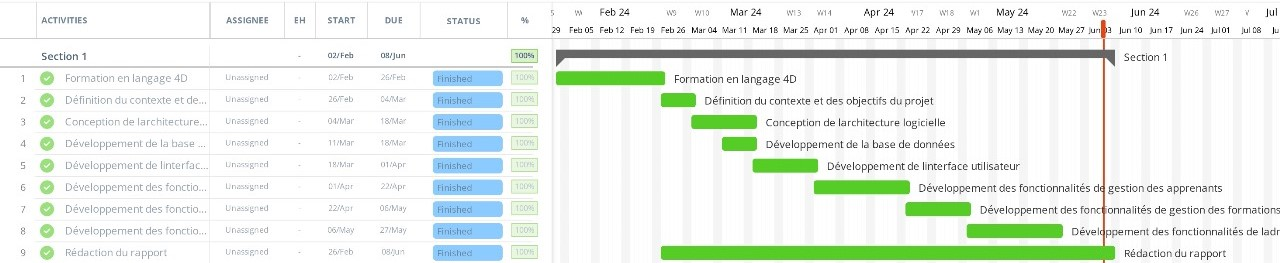
\includegraphics[width=18cm]{Figures/DiagrammeDeGantt.jpg}
%     \caption{Diagramme de Gantt.}
% \end{figure}

\begin{sidewaysfigure}
    \centering
    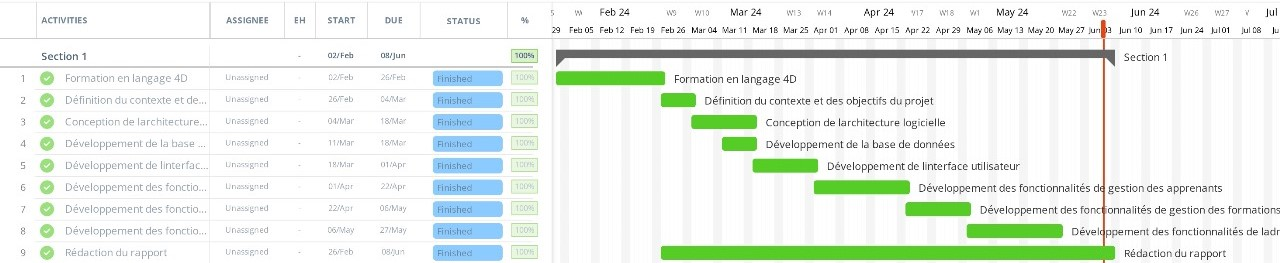
\includegraphics[width=\textheight,height=\textwidth,keepaspectratio]{Figures/DiagrammeDeGantt.jpg}
    \caption{Diagramme de Gantt.}
\end{sidewaysfigure}

\newpage
\subsection{Outils de collaboration:}

\subsubsection{Skype}

\begin{figure}[h]
    \centering
    
\includegraphics[scale=0.02]{Logos/Skype-Logo.png} % Replace with the actual filename of the IBM logo image
    \caption{Skype Logo}
\end{figure}

Skype est un logiciel propriétaire qui permet aux utilisateurs de passer des appels téléphoniques ou vidéo via Internet, ainsi que le partage d'écran. Les appels d’utilisateur à utilisateur sont gratuits, tandis que ceux vers les lignes téléphoniques fixes et les téléphones mobiles sont payants. Il existe des fonctionnalités additionnelles comme la messagerie instantanée, le transfert de fichiers et la visioconférence. 

Grâce à Skype, j'ai pu rester en contact régulier avec mon encadrant, mes collègues et les membres de l'entreprise. De plus, la fonction de partage d'écran de Skype a été extrêmement utile pour effectuer des présentations et des démonstrations de mon travail. Grâce à Skype, j'ai pu maintenir une communication fluide et efficace, ce qui a grandement contribué à la réussite de mon projet de fin d’étude.

\subsubsection{Git}

\begin{figure}[H]
    \centering
    
\includegraphics[scale=0.5]{Logos/git.png}
    \caption{Logo Git}
\end{figure}

Dans notre cas, et afin de conserver nos différentes versions du code source, nous avons
choisi de travailler avec Git comme logiciel de gestion de versions.

Git est un logiciel libre qui appartient au domaine publique (Licence GNU) et qui a
actuellement une communauté englobant près de 96\% des développeurs à travers le monde.

\subsubsection{GitLab}


\begin{figure}[H]
    \centering
    
\includegraphics[scale=0.1]{Logos/gitlab.jpg}
    \caption{Logo GitLab}
\end{figure}

Nous avons aussi opté pour GitLab, une plate-forme d'hébergement de code pour le
contrôle de version et la collaboration. Il permet, à nous et à d'autres, de travailler ensemble sur
des projets où que nous soyons.

\begin{figure}[H]
    \centering
    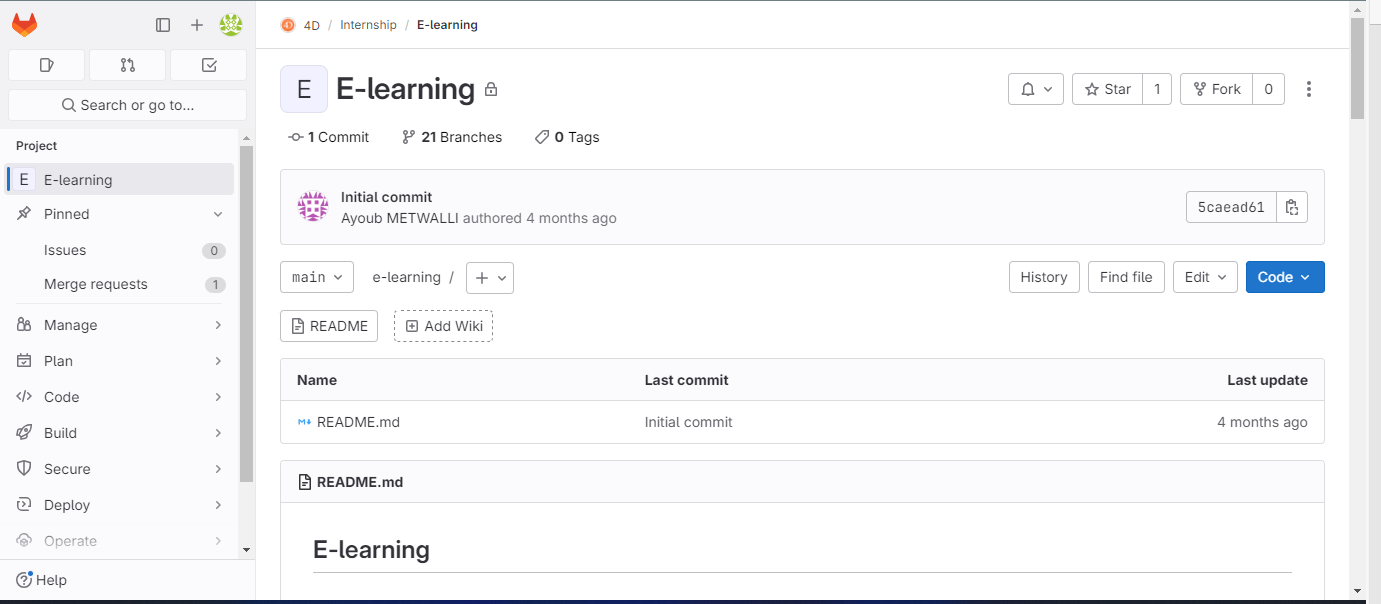
\includegraphics[width=19cm]{Figures/apercu.png}
    \caption{Aperçu globale de l'espace GitLab}
\end{figure}
\newpage

\section*{Conclusion}
Au cours de ce chapitre, nous avons mis l’accent sur le périmètre de notre projet. Nous avons éclairé
la méthodologie et le planning suivis pour mener ce projet. Nous entamerons dans le chapitre suivant
la phase d’analyse et spécification du système à développer au cours de laquelle nous comprenons en
profondeurs les besoins utilisateurs et construisons ainsi un système qui y répond.




\chapter{Analyse et spécification des besoins}
\label{chap:Analyse et spécification des besoins}



Dans ce chapitre, nous abordons l’étape d’analyse et spécification des besoins pour notre projet. Ainsi nous présentons en premier temps les acteurs ainsi que les exigences fonctionnelles et non-fonctionnelles du projet. Puis, nous utilisons les diagrammes de cas d’utilisations avec leurs descriptions textuelles pour décrire les scénarios possibles. Cela nous permettra de guider le développement du système de manière efficace et d’assurer sa conformité aux exigences.

\pagebreak

\section{Étude de l’existant}

Reconnu depuis 30 ans comme un partenaire privilégié du monde de l'éducation, 4D accompagne les directeurs d'établissements, les enseignants, les chercheurs et les responsables administratifs dans la réussite de leurs parcours. L'entreprise offre deux types de formation : la formation sur mesure et la formation standard. La formation sur mesure est adaptée spécifiquement aux besoins individuels de l'apprenant, permettant une personnalisation maximale du contenu et des méthodes d'enseignement. En revanche, la formation standard est une offre prédéfinie par l'entreprise, accessible à tout apprenant intéressé. Ces formations peuvent être suivies en ligne, à travers des plateformes telles que Zoom ou Google Meet, ou en présentiel, selon les modalités fixées par l'entreprise.

Avant la pandémie de COVID-19, la plupart des formations se déroulaient en mode présentiel. Cependant, avec la montée en puissance du travail à distance, les entreprises ont découvert qu'il était possible de tout faire en ligne. En conséquence, 4D a décidé de migrer vers les formations à distance. Cependant, l'utilisation des outils de visioconférences présente plusieurs limitations. La gestion des formations nécessite un grand effort manuel, et les formations ne sont pas regroupées dans un seul endroit où l'utilisateur peut consulter et choisir ce qui est adéquat pour ses besoins. la formation à travers ces outils n'est pas très productif pour l'apprenant. Il est donc nécessaire de trouver une solution plus efficace pour gérer et proposer les formations en ligne

\section{Spécification des exigences}

Cette phase de l’application vise à définir la frontière fonctionnelle entre le système et son environnement. Pour affiner les objectifs définis dans le contexte général du projet, il est essentiel de répondre à deux questions principales : Quels sont les utilisateurs du système ? Qu'attendent-ils de ce système ?

Pour trouver la réponse, nous avons opté pour la démarche suivante : 

- Définir les acteurs du système. 

- Lister ce que doit offrir le système à son utilisateur.


\subsection{Identification des acteurs}

Un acteur représente l’abstraction d’un rôle joué par des entités externes qui
interagissent directement avec le système étudié. Un acteur peut consulter et/ou
modifier directement l’état du système, en émettant et/ou en recevant des messages
susceptibles d'être porteur de données.

\begin{table}[htbp]
    \centering
    \begin{tabular}{|m{5cm}|m{10cm}|}
        \hline
        \textbf{Acteur} & \textbf{Rôle dans l'application} \\
        \hline
        Administrateur & Responsable de la gestion technique et opérationnelle de l'application, de la gestion des comptes des utilisateurs (Formateurs et Apprenants), de la sécurité des données et du support technique. Ainsi la création, gestion et mise à jour des cours. \\
        \hline
        Apprenant & Utilisateur principal de la plateforme, pouvant accéder aux cours, suivre les chapitres de formation, évaluer les contenus. \\
        \hline
    \end{tabular}
    \caption{Rôles dans l'application}
    \label{tab:roles}
\end{table}

\subsection{Exigences fonctionnelles}


\begin{itemize}
    \item[$\bullet$] \textbf{Authentification:} C’est l’étape primordiale pour toutes les fonctionnalités. Il s’agit de saisir un identifiant (email ou nom d'utilisateur) et un mot de passe puis de valider pour pouvoir exploiter les autres services.
    \item[$\bullet$] \textbf{Gestion des Abonnements:} Permettre aux apprenants de payer un abonnement pour accéder aux formations.
    \item[$\bullet$] \textbf{Gestion des Formations pour les Apprenants:}
    \begin{itemize}
        \item  S'inscrire à une formation: Permettre aux apprenants de s'inscrire à une formation après s'être authentifiés et avoir payé l'abonnement si nécessaire.
        \item  Consulter une formation: Permettre aux apprenants de consulter les détails d'une formation à laquelle ils sont inscrits.
        \item  Évaluer une formation: Permettre aux apprenants d'évaluer une formation après l'avoir suivie.
        \item  Chercher une formation: Permettre aux apprenants de rechercher des formations disponibles sur la plateforme.
        \item  Consulter le profil d'un formateur: Permettre aux apprenants de consulter les profils des formateurs sur la plateforme.
    \end{itemize}
    \item[$\bullet$] \textbf{Gestion des Profils Apprenants:}
    \begin{itemize}
        \item  Modifier son profil: Permettre aux apprenants de modifier leurs informations personnelles sur leur profil.
    \end{itemize}
    \item[$\bullet$] \textbf{Gestion des Formations pour les Administrateurs:}
    \begin{itemize}
        \item  Ajouter une formation: Permettre aux administrateurs d'ajouter une nouvelle formation sur la plateforme.
        \item  Modifier une formation: Permettre aux administrateurs de modifier une formation existante.
        \item  Supprimer une formation: Permettre aux administrateurs de supprimer une formation existante.
    \end{itemize}
    \item[$\bullet$] \textbf{Gestion des Apprenants pour les Administrateurs:}
    \begin{itemize}
        \item  Ajouter un apprenant: Permettre aux administrateurs d'ajouter un nouveau apprenant sur la plateforme.
        \item  Modifier un apprenant: Permettre aux administrateurs de modifier un apprenant existant.
        \item  Supprimer un apprenant: Permettre aux administrateurs de supprimer un apprenant existant.
    \end{itemize}
    \item[$\bullet$] \textbf{Gestion des Formateurs pour les Administrateurs:}
    \begin{itemize}
        \item  Ajouter un formateur: Permettre aux administrateurs d'ajouter un nouveau un formateur sur la plateforme.
        \item  Modifier un formateur: Permettre aux administrateurs de modifier un formateur existant.
        \item  Supprimer un formateur: Permettre aux administrateurs de supprimer un formateur existant.
    \end{itemize}
    \item[$\bullet$] \textbf{Gestion des Statistiques:}
    \begin{itemize}
        \item  Consulter les statistiques: Permettre aux administrateurs de consulter les statistiques de la plateforme.
    \end{itemize}
\end{itemize}


\subsection{Exigences non-fonctionnelles}


Ce sont les besoins qui permettent d’améliorer la qualité des services de la plateforme comme la convivialité et l’ergonomie des interfaces et l’amélioration du temps de réponse. Parmi ces besoins, on cite :

\begin{itemize}
    \item[$\bullet$] \textbf{Convivialité:} La future application doit être facile à utiliser. En effet, les interfaces utilisateur doivent être conviviales c’est-à-dire simples, ergonomiques et adaptées à l’utilisateur.
    \item[$\bullet$] \textbf{Scalabilité:} Toute architecture est exposée à des évolutions au niveau de la technologie d’implémentation. La solution doit avoir un grand niveau d’abstraction pour faciliter les nouvelles implémentations.
    \item[$\bullet$] \textbf{Performance:} Le temps de réponse doit être le plus court possible.
    \item[$\bullet$] \textbf{Disponibilité:} Lorsque n’importe quel utilisateur désire consulter la plateforme, elle doit être disponible.
    \item[$\bullet$] \textbf{Sécurité} la plateforme doit protéger les données personnelles des utilisateurs, garantir l'intégrité des cours et du contenu.
\end{itemize}

\section{Identification de cas d’utilisation}

\subsection{Diagramme de cas d’utilisation}

Les diagrammes de cas d'utilisation décrivent les fonctions générales et la portée d'un système. Ces diagrammes identifient également les interactions entre le système et ses acteurs.

Nous synthétisons dans ce paragraphe tout ce qui a été dit dans la phase d’analyse. Nous présentons le diagramme de cas d’utilisation de notre application et introduisons les cas d’utilisation qui le composent.

\begin{figure}[H]
    \centering
    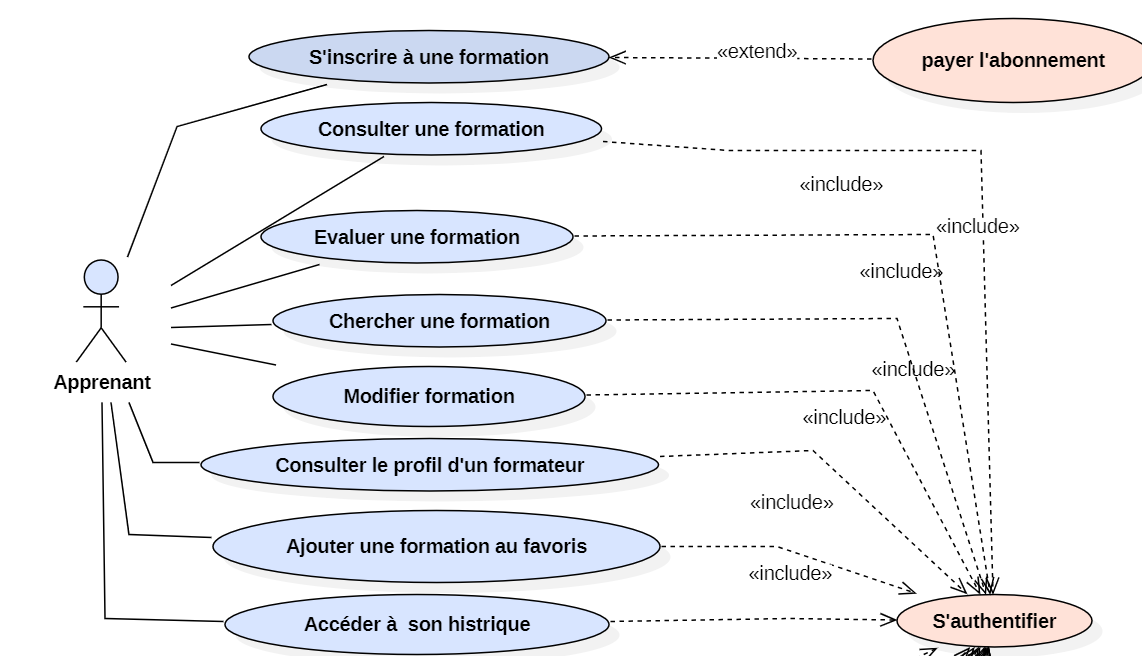
\includegraphics[width=15cm]{Figures/apprenant.PNG}
    \caption{Diagramme de cas d’utilisation d'apprenant}
\end{figure}

\begin{figure}[H]
    \centering
    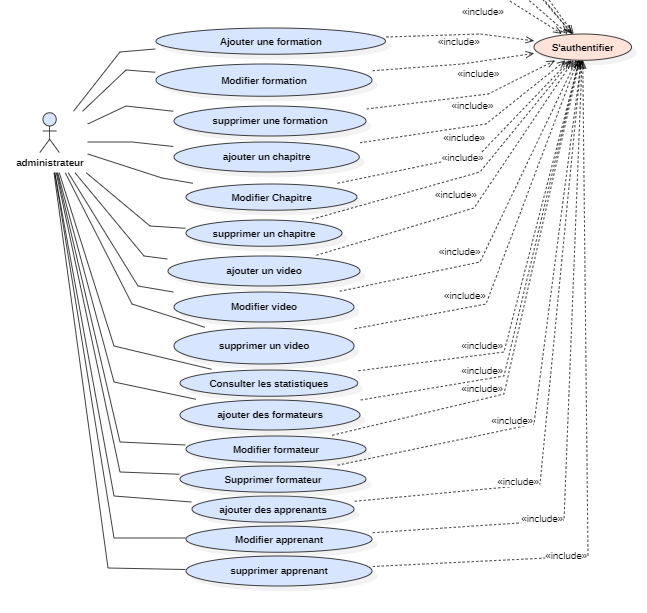
\includegraphics[width=13cm]{Figures/administrateur.PNG}
    \caption{Diagramme de cas d’utilisation d'administrateur}
\end{figure}

\subsection{Description textuelle de cas d’utilisation}

\begin{minipage}{\textwidth}
\begin{table}[H]
\centering
\begin{tabular}{| m{8cm} | m{8cm} |}
\hline
\multicolumn{2}{|c|}{\textbf{UC 1:} Payer l'abonnement d'une formation} \\ \hline
\textbf{Acteurs} & Utilisateur \\ \hline
\textbf{But} & Permettre à un utilisateur d'accéder à une formation disponible sur la plateforme et voir les vidéos \\ \hline
\textbf{Préconditions} & \textbf{Postconditions} \\ \hline
- S'authentifier. & - Voir les vidéos \\ \hline
\textbf{Scénario Principal} & \textbf{Scénario Alternatif} \\ \hline
\begin{enumerate}
    \item S'authentifier.
    \item Naviguer vers la page de la formation.
    \item Choisir la formation.
    \item Cliquer sur "S'inscrire".
    \item Effectuer le paiement.
    \item Si le paiement est autorisé.
    \item Le client est redirigé vers la page de confirmation de paiement.
\end{enumerate} & 
\begin{enumerate}
    \item S'authentifier.
    \item Naviguer vers la page de la formation.
    \item Choisir la formation.
    \item Cliquer sur "S'inscrire".
    \item Effectuer le paiement.
    \item Si le paiement n'est pas autorisé.
    \item Le client est redirigé vers la page d’erreur.
\end{enumerate} \\ \hline
\end{tabular}
\caption{Description Textuelle du Cas d'Utilisation "Payer l'abonnement d'une formation"}
\label{tab:use_case_description_1}
\end{table}
\end{minipage}

\newpage

\begin{minipage}{\textwidth}
\begin{table}[H]
\centering
\begin{tabular}{| m{8cm} | m{8cm} |}
\hline
\multicolumn{2}{|c|}{\textbf{UC 2:} Ajouter une formation} \\ \hline
\textbf{Acteurs} & Administrateur \\ \hline
\textbf{But} & Permettre à un administrateur d'ajouter une formation à la plateforme avec ses chapitres et ses vidéos \\ \hline
\textbf{Préconditions} & \textbf{Postconditions} \\ \hline
- S'authentifier. & - \\ \hline
\textbf{Scénario Principal} & \textbf{Scénario Alternatif} \\ \hline
\begin{enumerate}
    \item S'authentifier.
    \item Naviguer vers la page d'ajout de formation.
    \item Remplir les informations nécessaires pour la formation.
    \item Ajouter les chapitres.
    \item Ajouter les vidéos.
    \item Cliquer sur le bouton "Enregistrer".
    \item Un message de confirmation est affiché.
\end{enumerate} & 
\begin{enumerate}
    \item S'authentifier.
    \item Naviguer vers la page d'ajout de formation.
    \item Remplir les informations nécessaires pour la formation.
    \item Ajouter les chapitres.
    \item Ajouter les vidéos.
    \item Cliquer sur le bouton "Enregistrer".
    \item Un message d'erreur spécifiant les champs incorrects ou manquants est affiché.
\end{enumerate} \\ \hline
\end{tabular}
\caption{Description Textuelle du Cas d'Utilisation "Ajouter une formation"}
\label{tab:use_case_description_2}
\end{table}
\end{minipage}

\newpage

\begin{minipage}{\textwidth}
\begin{table}[H]
\centering
\begin{tabular}{| m{8cm} | m{8cm} |}
\hline
\multicolumn{2}{|c|}{\textbf{UC 3:} Ajouter un chapitre} \\ \hline
\textbf{Acteurs} & Administrateur \\ \hline
\textbf{But} & Permettre à un administrateur d'ajouter un chapitre à une formation existante \\ \hline
\textbf{Préconditions} & \textbf{Postconditions} \\ \hline
- S'authentifier. & - \\ \hline
\textbf{Scénario Principal} & \textbf{Scénario Alternatif} \\ \hline
\begin{enumerate}
    \item S'authentifier.
    \item Naviguer vers la page des formations.
    \item Remplir les informations nécessaires pour le chapitre.
    \item Ajouter les vidéos.
    \item Cliquer sur le bouton "Enregistrer".
    \item Un message de confirmation est affiché.
\end{enumerate} & 
\begin{enumerate}
    \item S'authentifier.
    \item Naviguer vers la page des formations.
    \item Remplir les informations nécessaires pour le chapitre.
    \item Ajouter les vidéos.
    \item Cliquer sur le bouton "Enregistrer".
    \item Un message d'erreur spécifiant les champs incorrects ou manquants est affiché.
\end{enumerate} \\ \hline
\end{tabular}
\caption{Description Textuelle du Cas d'Utilisation "Ajouter un chapitre"}
\label{tab:use_case_description_3}
\end{table}
\end{minipage}

\newpage

\begin{minipage}{\textwidth}
\begin{table}[H]
\centering
\begin{tabular}{| m{8cm} | m{8cm} |}
\hline
\multicolumn{2}{|c|}{\textbf{UC 4:} Ajouter un apprenant} \\ \hline
\textbf{Acteurs} & Administrateur \\ \hline
\textbf{But} & Permettre à un administrateur d'ajouter un apprenant pour qu'il puisse s'authentifier à la plateforme. \\ \hline
\textbf{Préconditions} & \textbf{Postconditions} \\ \hline
- S'authentifier. & - \\ \hline
\textbf{Scénario Principal} & \textbf{Scénario Alternatif} \\ \hline
\begin{enumerate}
    \item S'authentifier.
    \item Naviguer vers la page des apprenants.
    \item Remplir les informations nécessaires pour l'apprenant.
    \item Cliquer sur le bouton "Enregistrer".
    \item Un message de confirmation est affiché.
\end{enumerate} & 
\begin{enumerate}
    \item S'authentifier.
    \item Naviguer vers la page des apprenants.
    \item Remplir les informations nécessaires pour l'apprenant.
    \item Cliquer sur le bouton "Enregistrer".
    \item Un message d'erreur spécifiant les champs incorrects ou manquants est affiché.
\end{enumerate} \\ \hline
\end{tabular}
\caption{Description Textuelle du Cas d'Utilisation "Ajouter un apprenant"}
\label{tab:use_case_description_4}
\end{table}
\end{minipage}

\clearpage

\section*{Conclusion}

La phase d’analyse est critique pour le succès d’un projet logiciel. Nous avons abordé cette phase en identifiant les acteurs et les cas d’utilisations, et nous avons représenté notre analyse en utilisant un diagramme de cas d’utilisations accompagné par des descriptions textuelles. Nous enchaînerons par la suite sur la conception du projet.


\chapter{Conception de la solution}
\label{Conception de la solution}



Dans cette partie, nous allons commencer d’abord par le prototype de notre application. Ensuite, nous allons se concentrer sur la  vue architecturale du projet.Finalement, nous allons détailler la conception en présentant les
diagrammes de séquence et les diagrammes de classe. Ces diagrammes permettent de visualiser les différentes étapes du processus et la structure du système.

\pagebreak
\section{Prototypage}

Le prototypage est une étape importante dans le processus de développement de notre application. Il permet de créer une version préliminaire de
 l'application pour tester ces fonctionnalités, recueillir des retours utilisateurs, et identifier d'éventuelles améliorations avant de passer à la phase de développement complète.

 Dans cette section, nous décrirons les étapes de création du prototype

\subsection{Choix de l'outil}

\begin{figure}[H]
    \centering
    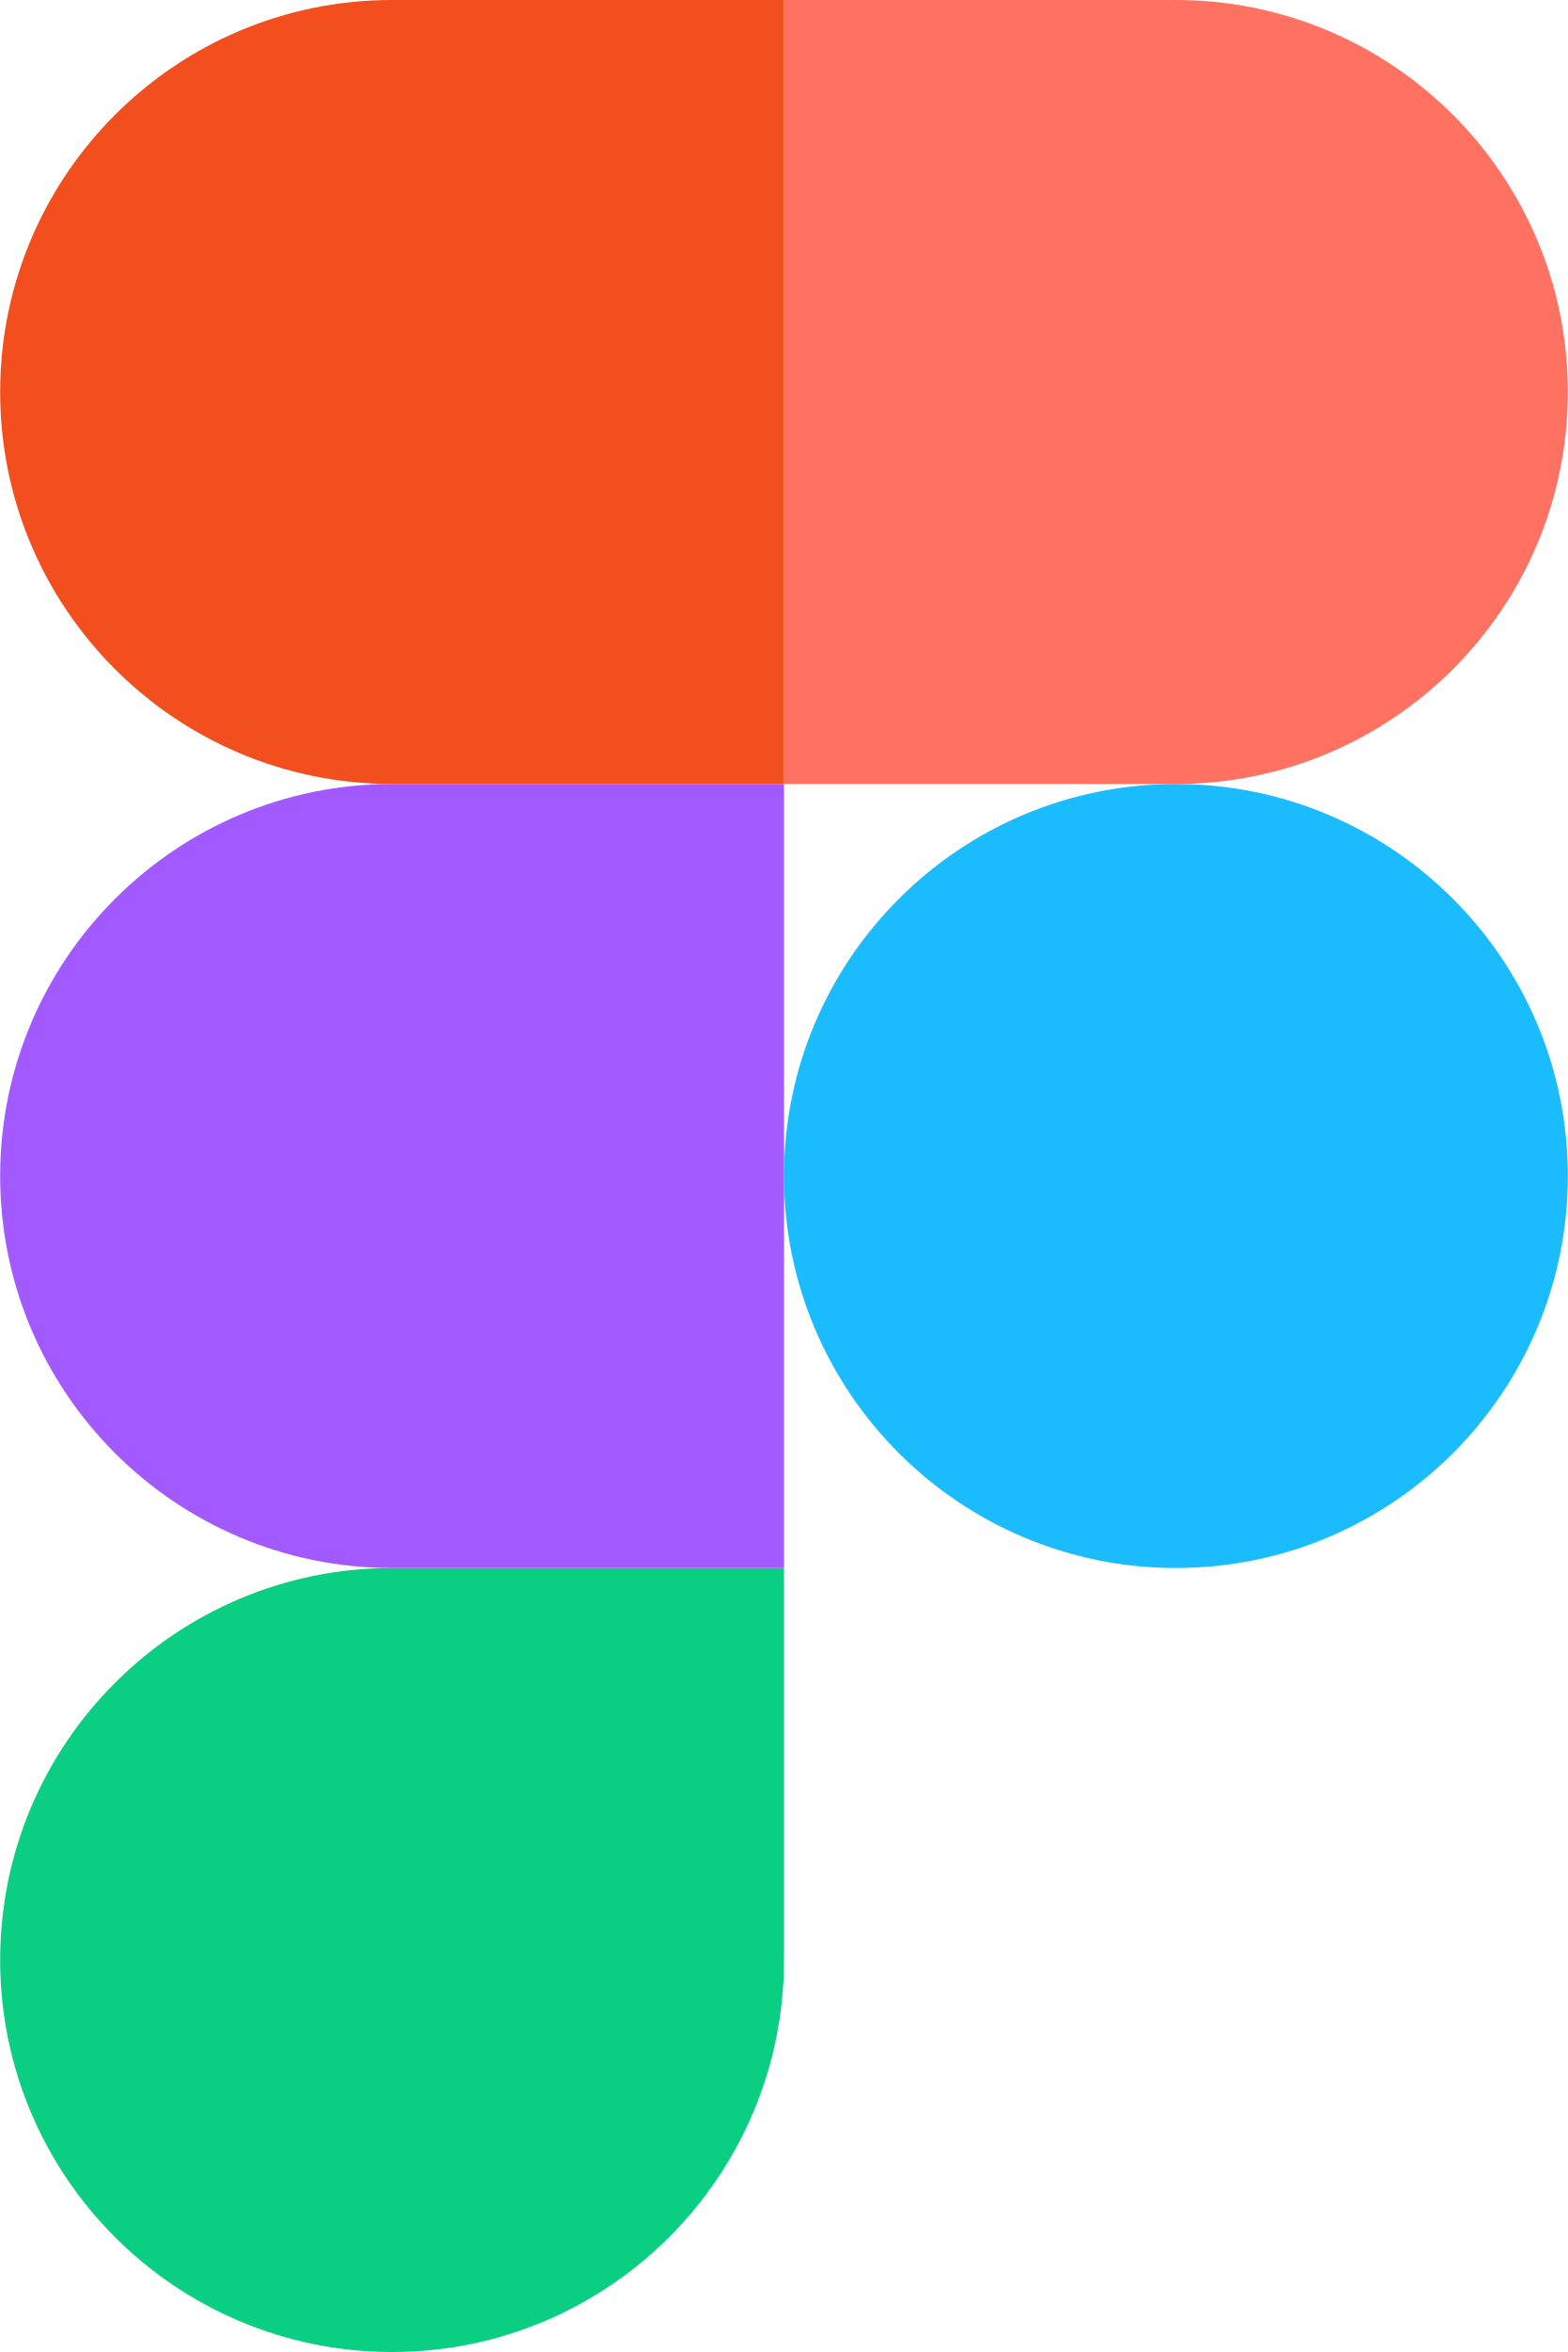
\includegraphics[scale=0.05]{Logos/Figma.png}
    \caption{Logo Figma}
\end{figure} 

Figma est une plateforme collaborative pour éditer des graphiques vectoriels et faire du prototypage. Elle permet de concevoir des design systems pour faciliter la création de sites web et d’applications mobiles. C’est une solution à destination des UI et UX designers et des développeurs. L’interface propose de nombreuses fonctionnalités :

\begin{itemize}
    \item[$\bullet$] \textbf{Design:} avec des outils de conception pour le web, des fonctions de mise en page automatique, des plugins pour réduire les tâches répétitives.
    \item[$\bullet$] \textbf{Prototypage:} pour tester les concepts très tôt en cours de design.
    \item[$\bullet$] \textbf{Design system:} pour concevoir des design cohérents avec des bibliothèques mises à jour en permanence.
    \item[$\bullet$] \textbf{Collaboration:} pour travailler à plusieurs et en même temps sur un projet, revenir sur une version antérieure si nécessaire ou encore afficher le travail d’un seul collaborateur par exemple.
\end{itemize}

\subsection{Interface}

\subsubsection{Espace apprenant}

\begin{figure}[H]
    \centering
    \begin{minipage}{0.45\textwidth}
        \centering
        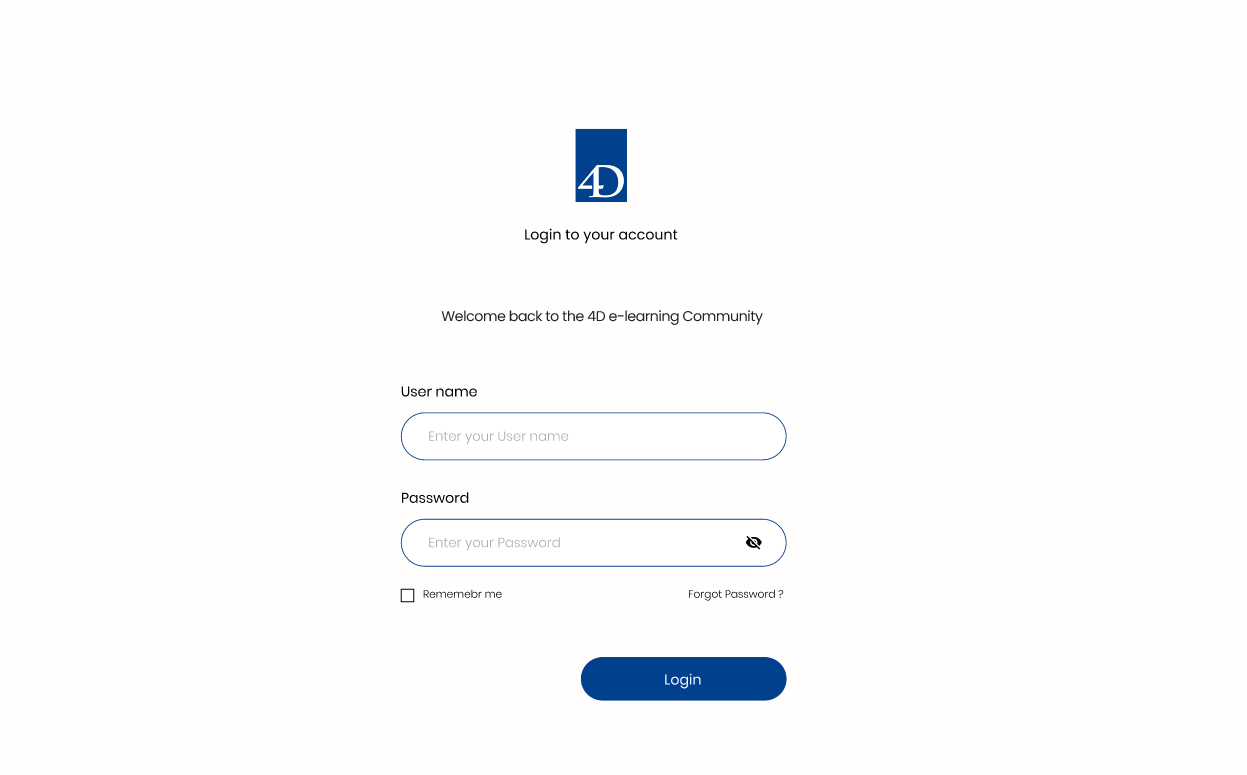
\includegraphics[width=\textwidth]{Figures/login.PNG}
        \caption{Figma: Page Login}
    \end{minipage}
    \hfill
    \begin{minipage}{0.45\textwidth}
        \centering
        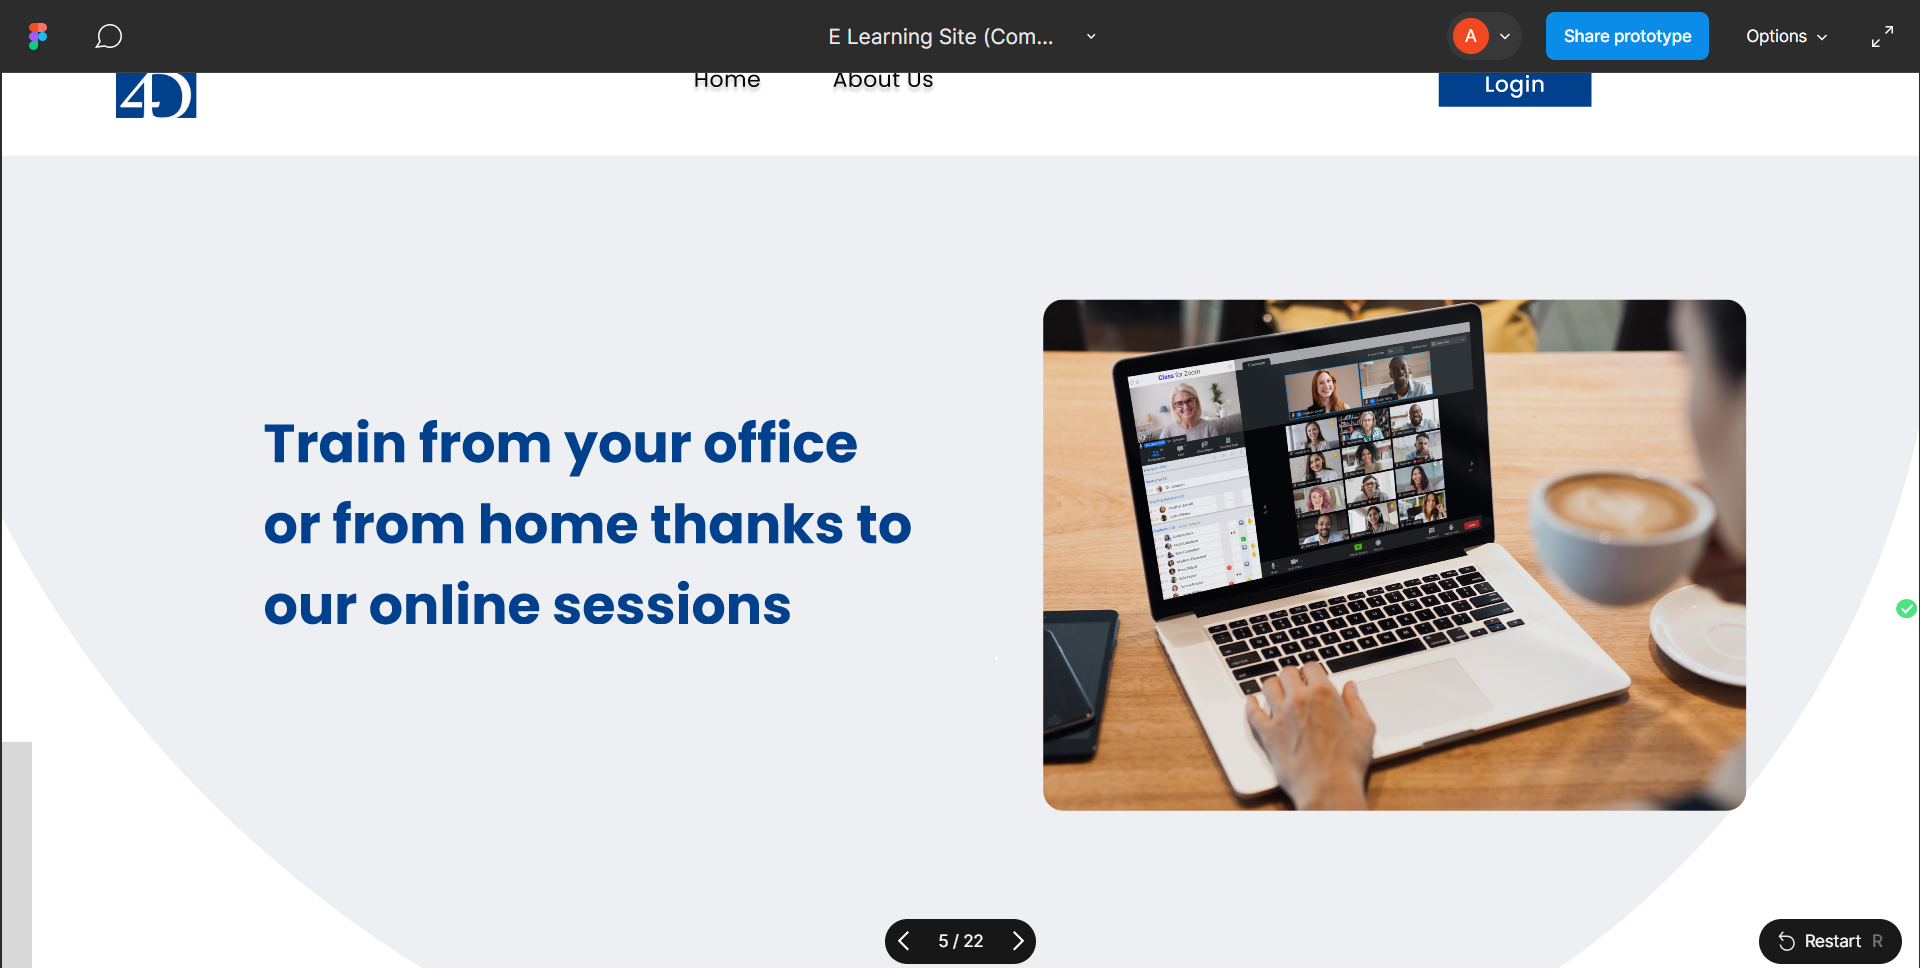
\includegraphics[width=\textwidth]{Figures/home.PNG}
        \caption{Figma: Page Home}
    \end{minipage}
\end{figure}

\begin{figure}[H]
    \centering
    \begin{minipage}{0.45\textwidth}
        \centering
        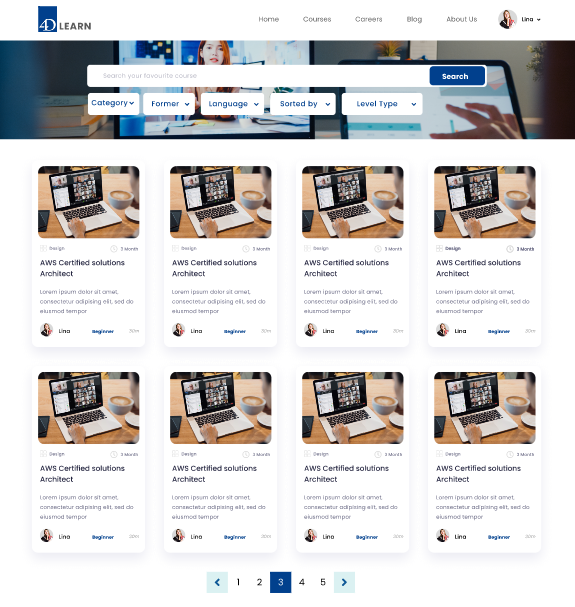
\includegraphics[width=\textwidth]{Figures/explorer.PNG}
        \caption{Figma: Page des Formations}

    \end{minipage}
    \hfill
    \begin{minipage}{0.45\textwidth}
        \centering
        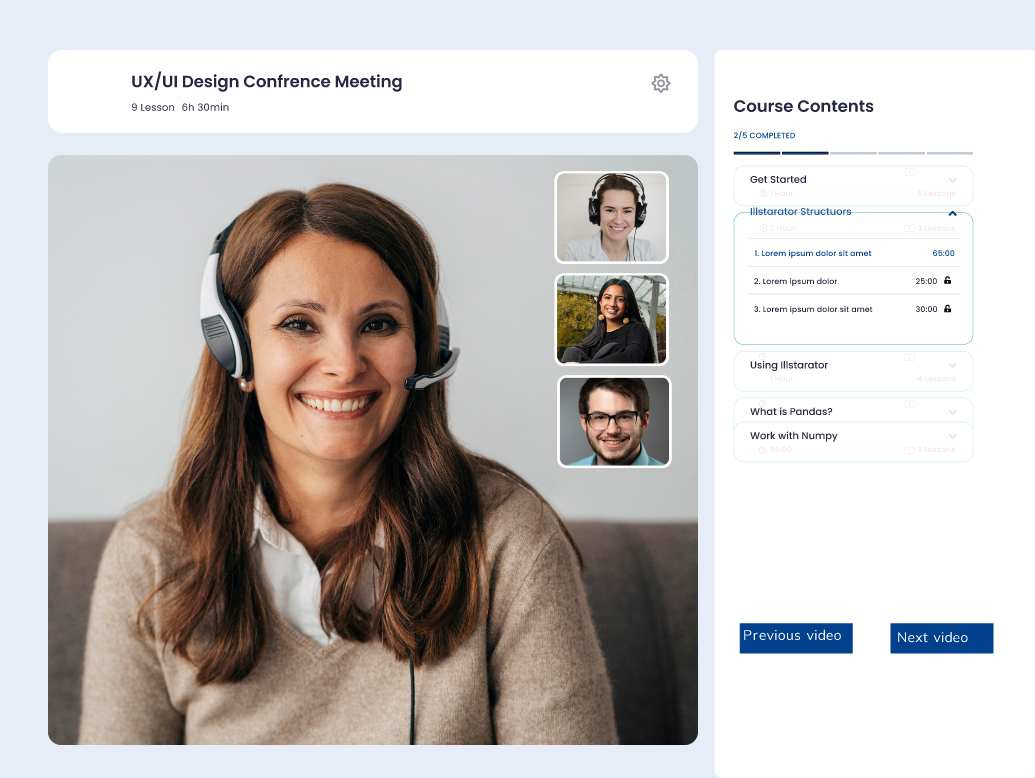
\includegraphics[width=\textwidth]{Figures/watchVideo.PNG}
        \caption{Figma: Page Suivre Formation }
        
    \end{minipage}
\end{figure}


\begin{figure}[H]
    \centering
    \begin{minipage}{0.45\textwidth}
        \centering
        
\includegraphics[width=\textwidth]{Figures/overview.PNG}
        \caption{Figma: Page Overview}
    \end{minipage}
    \hfill
    \begin{minipage}{0.45\textwidth}
        \centering
        
\includegraphics[width=\textwidth]{Figures/Chapter.PNG}
        \caption{Figma: Page des Chapitres }
    \end{minipage}
    
\end{figure}

\begin{figure}[H]
    \centering
    \begin{minipage}{0.45\textwidth}
        \centering
        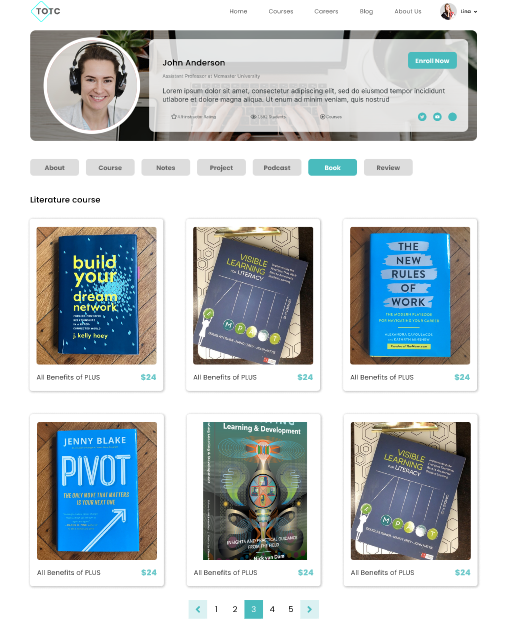
\includegraphics[width=\textwidth]{Figures/AuthorDetails.PNG}
        \caption{Figma: Page Détails d'un Formateur}
    \end{minipage}
    \hfill
    \begin{minipage}{0.45\textwidth}
        \centering
        
\includegraphics[width=\textwidth]{Figures/comment.PNG}
        \caption{Figma: Page des Chapitres}
    \end{minipage}
    
\end{figure}

\subsubsection{Espace administrateur}

\begin{figure}[H]
    \centering
    \begin{minipage}{0.45\textwidth}
        \centering
        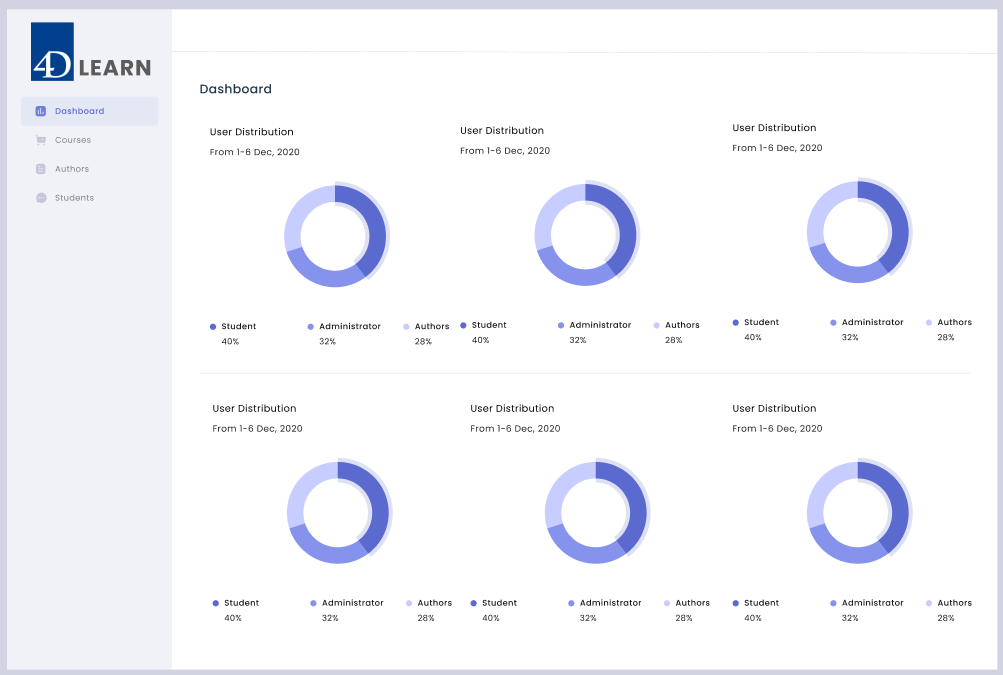
\includegraphics[width=\textwidth]{Figures/figmaDashoboard.PNG}
        \caption{Figma: Page Tableau De Board}
    \end{minipage}
    \hfill
    \begin{minipage}{0.45\textwidth}
        \centering
        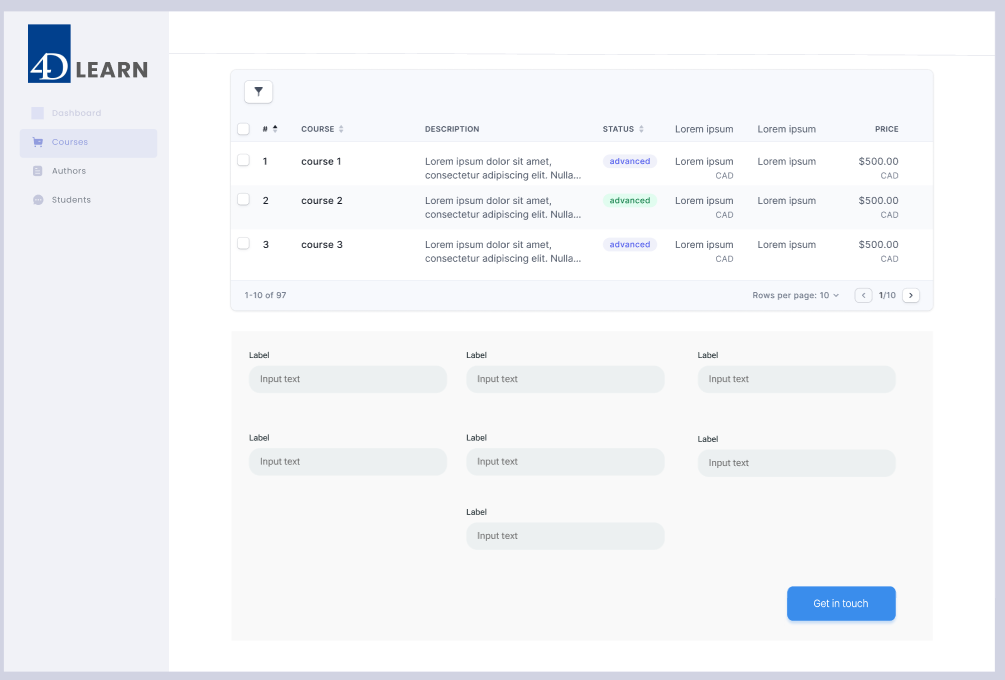
\includegraphics[width=\textwidth]{Figures/addCourseDashboard.png}
        \caption{Figma: Page D'ajout De Formation}
    \end{minipage}
    
\end{figure}

\section{Architecture de l’application}

\subsection{Architecture physique}

Nous avons opté pour l’architecture client/serveur multi-tiers. En effet, l’accès à l’application exige le passage à
travers des requêtes HTTP afin de récupérer et de déposer des versions dans le dépôt
central. De plus, la gestion de la base de données du système doit être centralisée et délocalisée de l’endroit de la couche métier, ce qui aide à garder une aisance de maintenance.
Et enfin, il faut que l’application soit distribuée sur plusieurs serveurs et chaque serveur
s’occupe d’une tâche. En effet, grâce au partage des tâches entre les différents serveurs,
nous pourrons garantir une grande souplesse, des bonnes performances et un temps de
réponse réduit. La figure suivante illustre l’architecture physique que nous avons :

\begin{figure}[H]
    \centering
    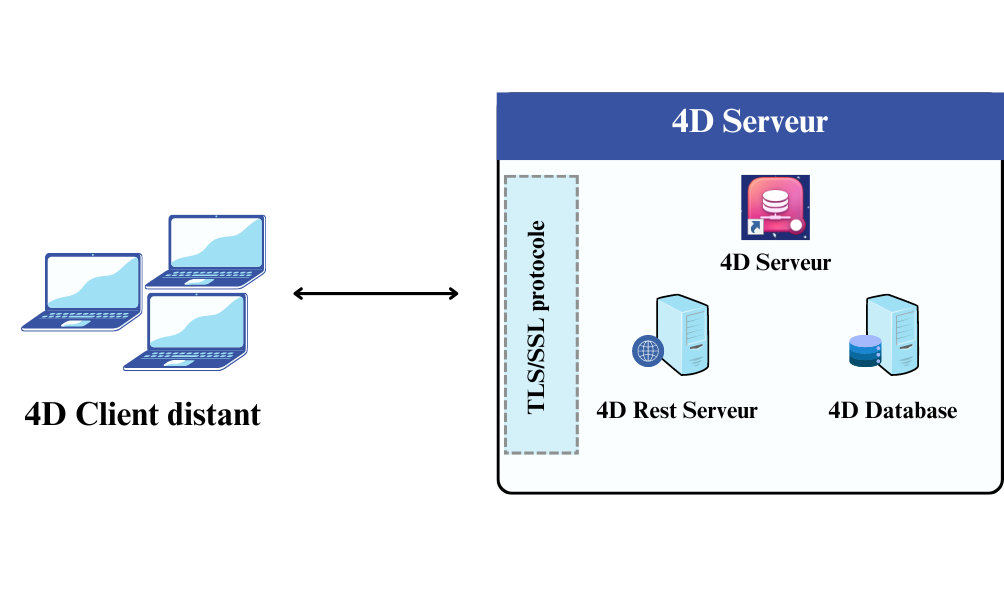
\includegraphics[width=15cm]{Figures/architecturePhysique.png}
    \caption{Architecture physique de système.}
\end{figure}

Cette architecture se compose principalement des éléments suivants :

\begin{itemize}
    \item[$\bullet$] \textbf{Serveur REST} : Un serveur web qui suit les principes de l'architecture REST et expose des ressources via des URI, permettant aux clients d'effectuer des opérations standardisées sur ces ressources pour accéder aux données et fonctionnalités du serveur.
    \item[$\bullet$] \textbf{Serveur 4D} : Ce serveur contient la couche métier de notre application.
    \item[$\bullet$] \textbf{Serveur de base de données} : Ce serveur se charge de la gestion du stockage des données.
    \item[$\bullet$] \textbf{Couche réseau} : Le protocole TLS sécurise les connexions client/serveur en cryptant les données échangées, permettant ainsi de renforcer la sécurité de notre application 4D Server.
\end{itemize}

\subsection{Architecture logique}

Dans notre architecture, nous avons utilisé le principe
de « Couche » pour séparer au maximum les différents types de traitement de l’application. L’environnement de travail n’est pas dépendant à une technologie spécifique.
Pour cette raison, nous avons utilisé plusieurs technologies afin de développer une solution multicouches  qui s’intègre parfaitement. La figure suivante
illustre l’architecture logicielle proposée pour le système développé, en présentant quatre
couches: couche présentation, couche controlleur, couche métier qui s’occupe des différents traitements
et couche accès aux données.


\begin{figure}[H]
    \centering
    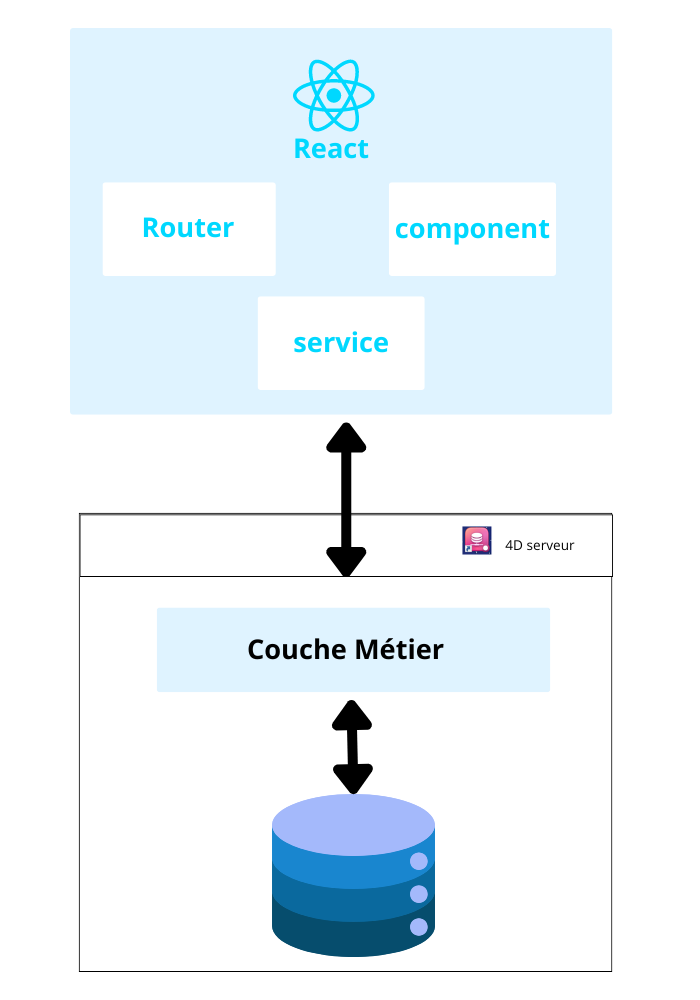
\includegraphics[width=9cm]{Figures/architectureLogique.png}
    \caption{Architecture logique de système.}
\end{figure}

Au niveau 4D Server, notre développement s’est concentré principalement sur la couche
métier. En effet, 4D Server offre un environnement de développement qui simplifie considérablement la création d’applications. Les autres couches, telles que la couche d’accès
aux données et la couche controlleur, sont déjà implémentées et intégrées dans 4D.Ainsi, les développeurs peuvent se concentrer sur la logique métier de leurs applications
sans avoir à se soucier des détails techniques des autres couches. Cette approche permet
un développement rapide et efficace, tout en offrant des fonctionnalités avancées pour
répondre aux besoins spécifiques des projets.

Aussi, nous avons travaillé avec ORDA (Object Relational Data Access), qui est une technologie spécifique qui facilite
l’accès à une base de données relationnelle en tant qu’objets. Elle permet de manipuler les
données de la base de données à l’aide d’un langage de programmation orienté objet ou
d’interfaces utilisateur spécifiques. ORDA simplifie l’interaction avec la base de données
en fournissant des abstractions supplémentaires et en masquant certaines complexités liées
aux requêtes SQL.

ORDA nous permet de créer des fonctions de classe de haut niveau au-dessus du modèle de données. Cela nous permet d'écrire du code orienté métier et de le «publier» comme une API. Le datastore, les dataclasses, les entity selections et les entités sont tous disponibles en tant qu'objets de classe pouvant contenir des fonctions.

\begin{figure}[H]
    \centering
    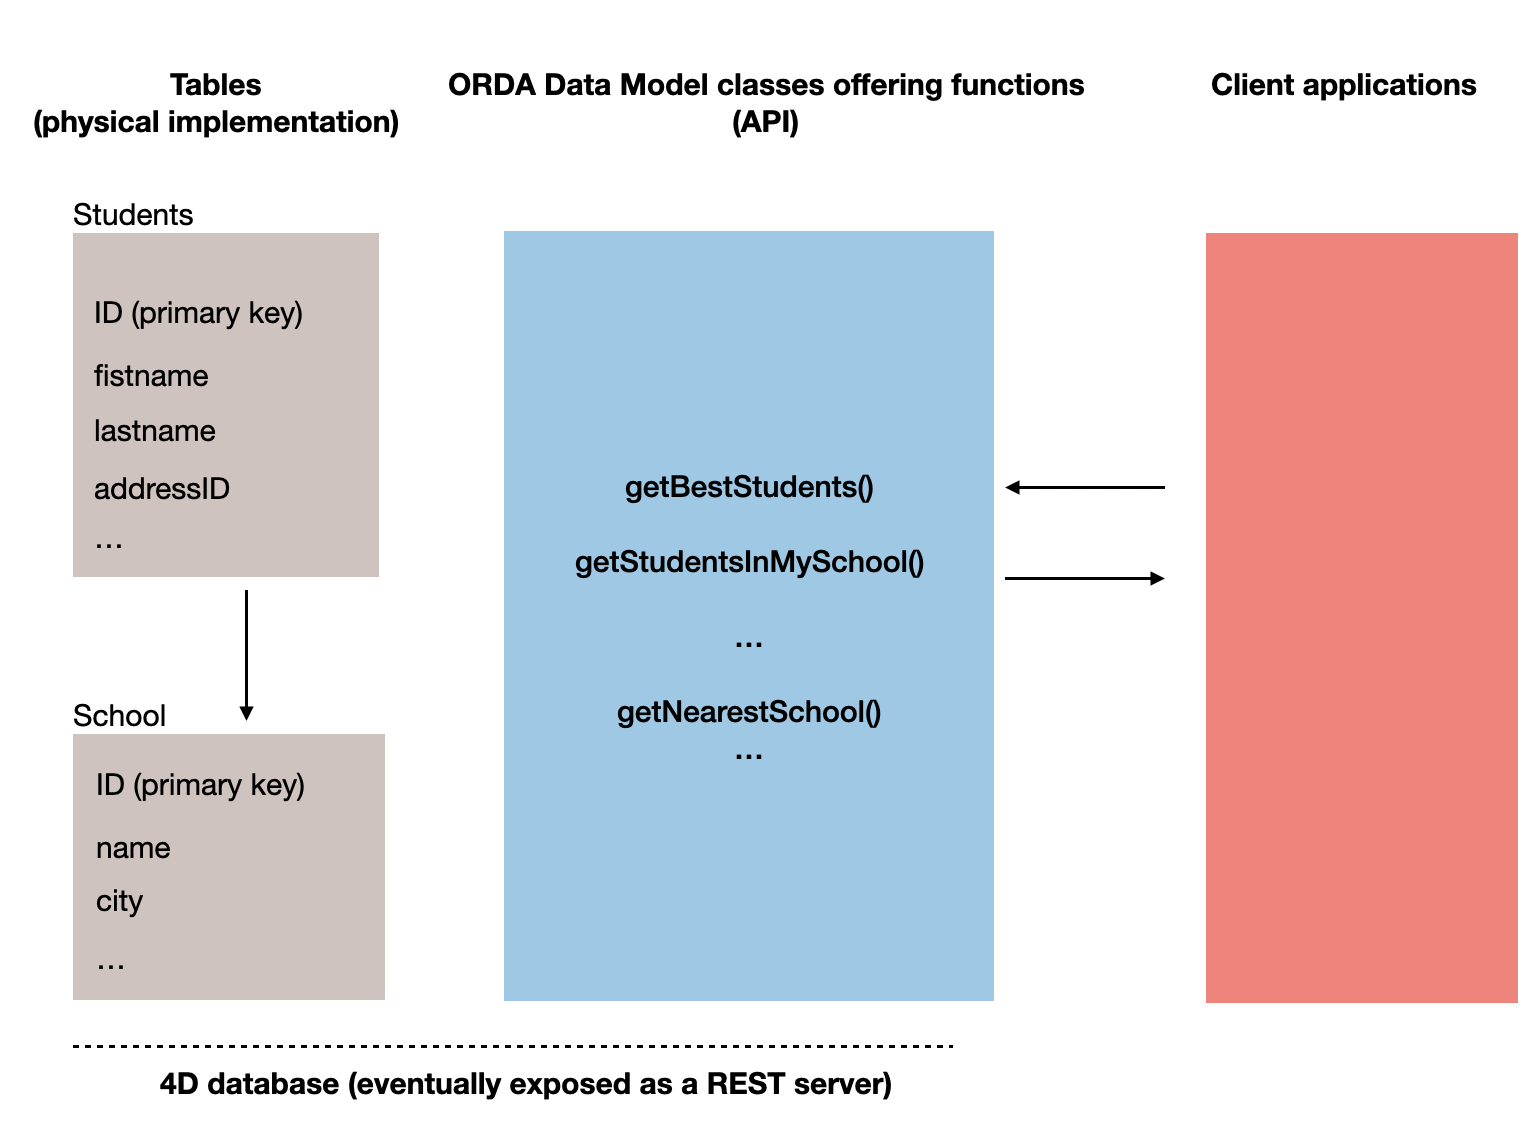
\includegraphics[width=15cm]{Figures/orda.png}
    \caption{Orda Data Model Class}
\end{figure}

Grâce à 4D, les développeurs peuvent se concentrer sur l’essentiel et créer des applications puissantes et performantes en toute simplicité.


\section{Conception Détaillée}

\subsection{Diagramme de Classe}
Le diagramme de classe est l’un des diagrammes statiques d’UML. Il permet de décrire
la structure d’un système informatique tout en montrant les différentes classes, leurs
attributs, leurs méthodes ainsi que les relations entre eux.

\begin{figure}[H]
    \centering
    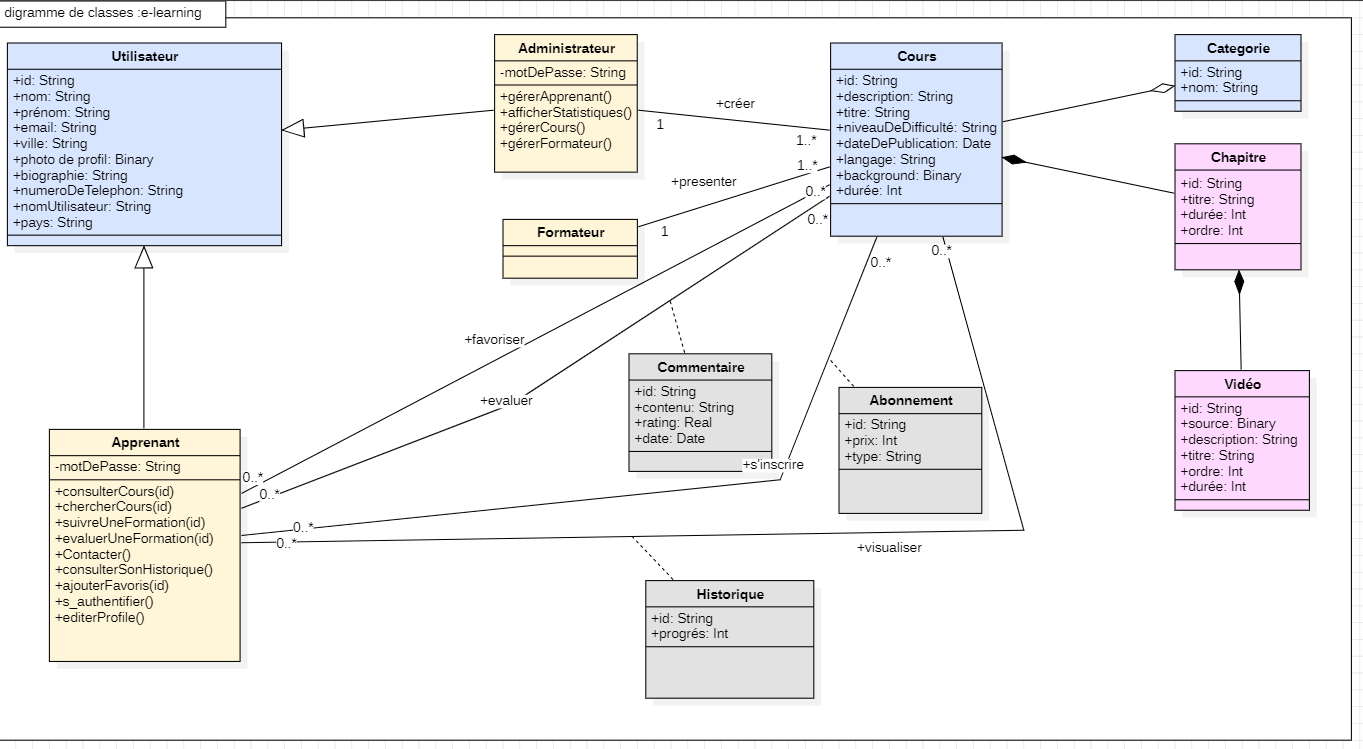
\includegraphics[width=19cm]{Figures/diagramme de classe.PNG}
    \caption{Diagramme de Classe}
\end{figure}

\subsection{Diagramme de séquence détaillé}

\subsubsection*{Diagramme de séquence de l'authentification}

Dans ce diagramme, nous avons essayé de montrer de manière plus détaillée comment un utilisateur peut s'identifier sur notre plateforme.

\begin{figure}[H]
    \centering
    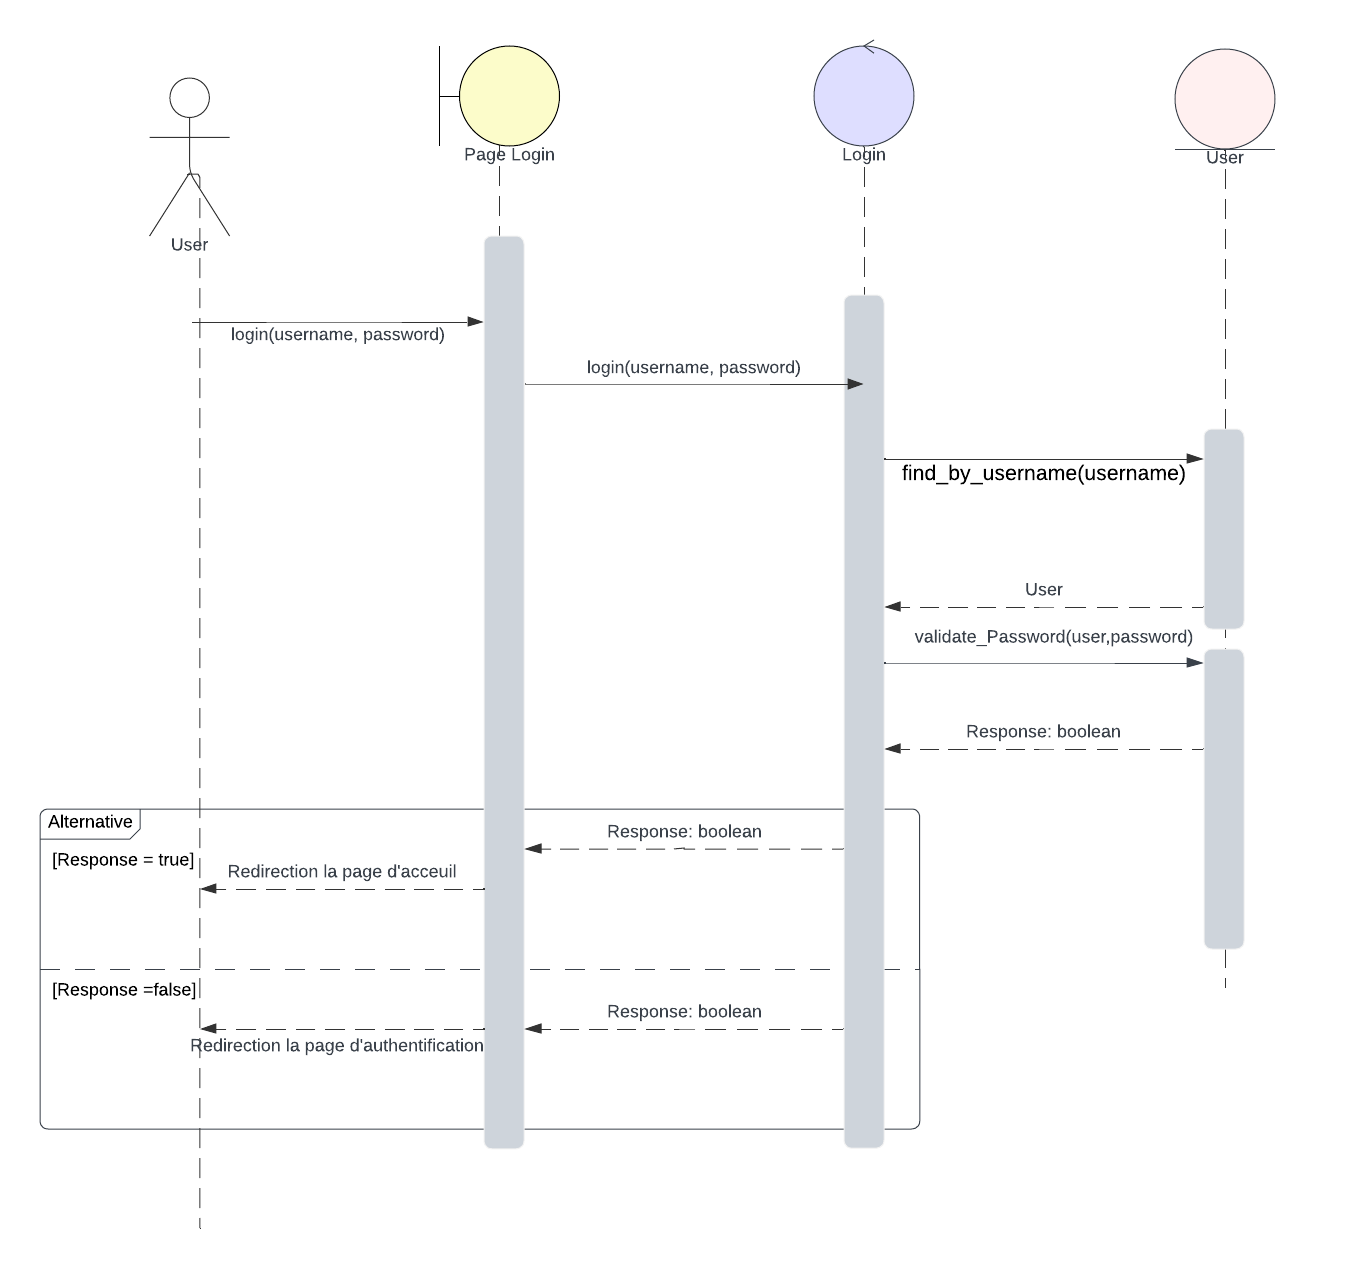
\includegraphics[width=19cm]{Figures/authdetaille.png}
    \caption{Diagramme de séquence détaillé de l'authentification}
\end{figure}

\subsubsection*{Diagramme de séquence d’ajouter une formation}

Ce diagramme montre comment le système ajoute une formation. D'abord, après avoir cliqué sur le bouton "Add Course", le système essaie d'abord d'enregistrer les informations de la formation. Ensuite, grâce à l'ID de la formation, on peut ajouter les chapitres liés à cette formation, ainsi que les vidéos. Tout cela se fait de manière transactionnelle pour s'assurer que le cours est ajouté correctement. 

\begin{figure}[H]
    \centering
    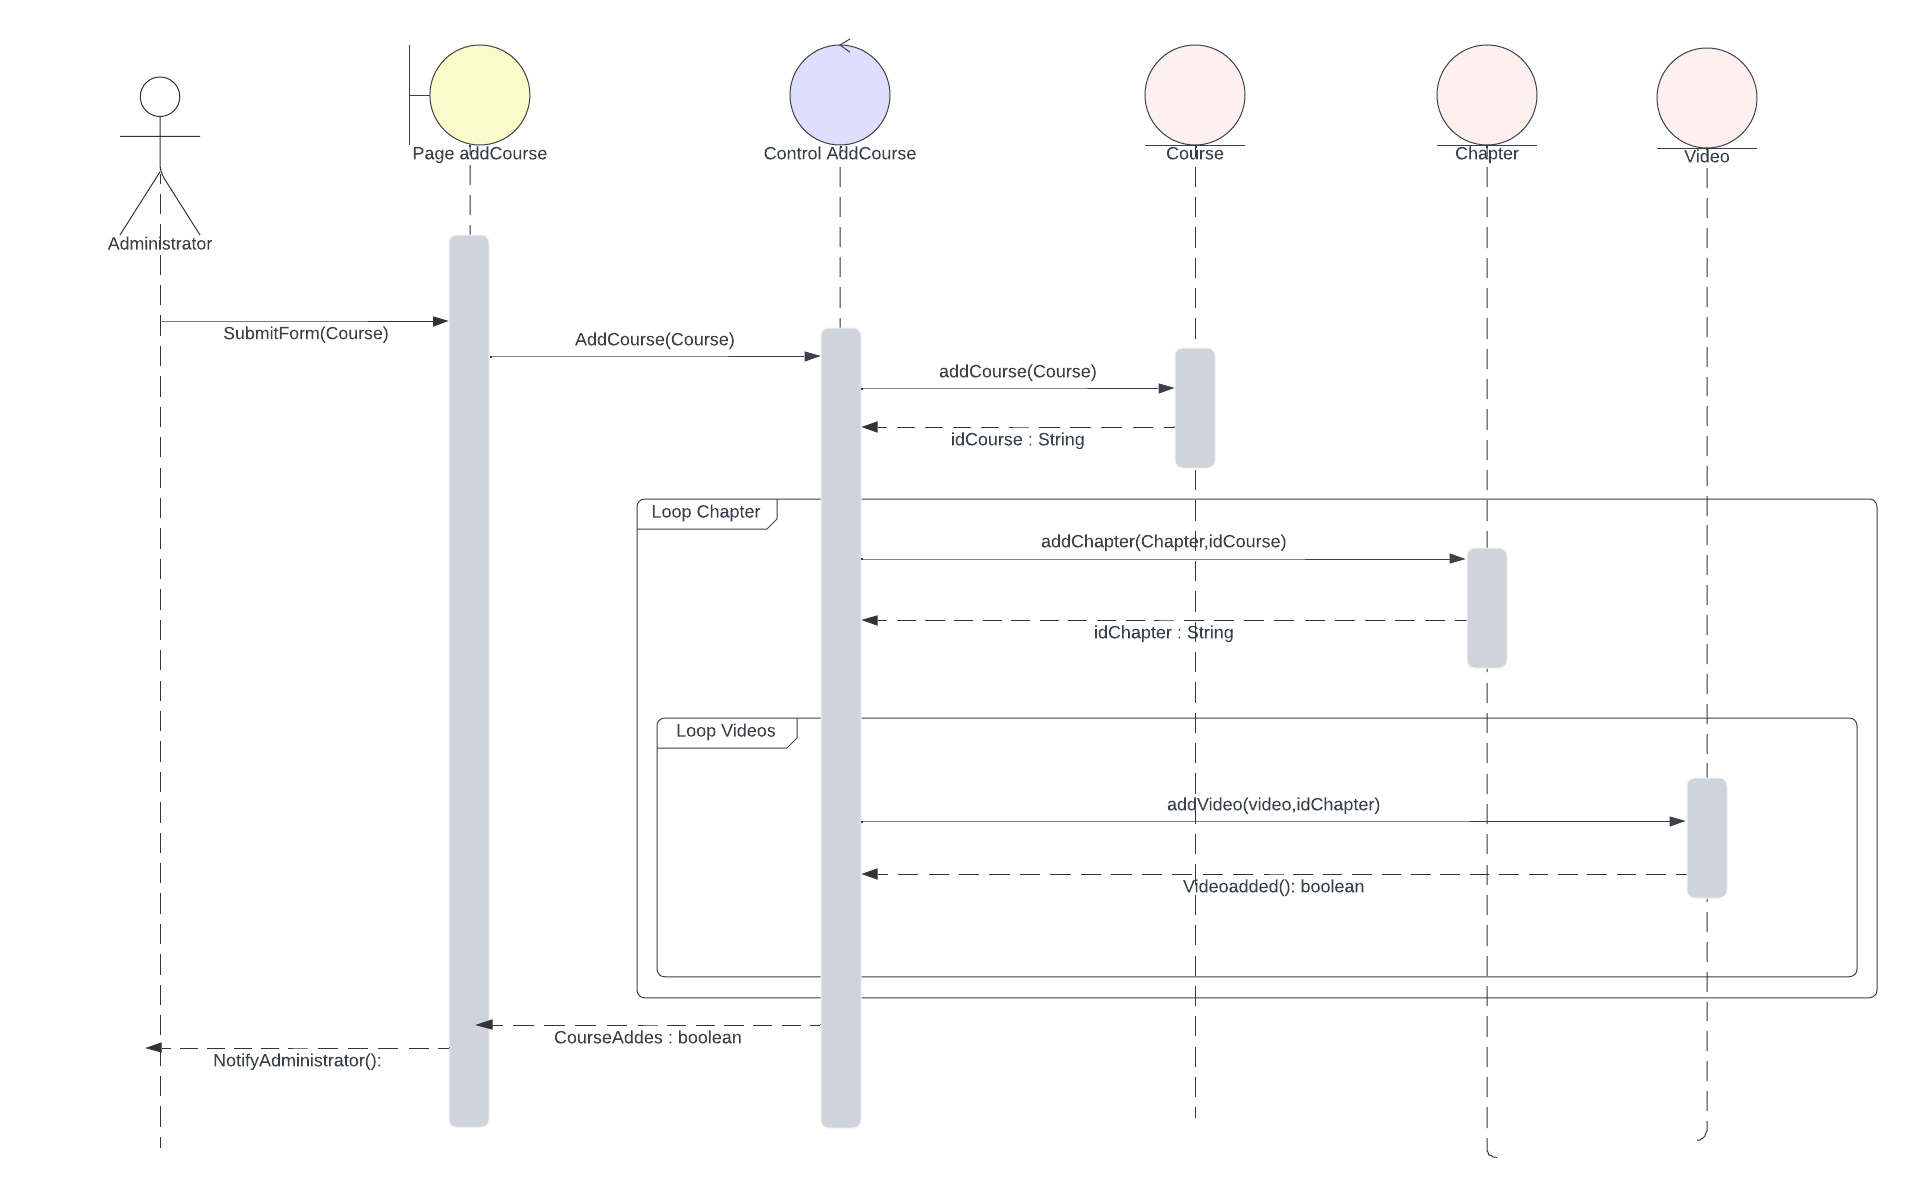
\includegraphics[width=19cm]{Figures/addcourseSequence.png}
    \caption{Diagramme de séquence détaillé d’ajouter une formation}
\end{figure}
\newpage
\subsection*{Conclusion}
Au cours de ce chapitre, nous avons d'abord présenté le prototype de notre application. Ensuite, nous avons examiné les architectures utilisées ainsi que les diagrammes de classes et de séquences. Nous allons maintenant entamer la partie de l'implémentation et la validation de notre solution.


\chapter{Réalisation}
\label{chap:Réalisation}


Dans ce chapitre, nous présentons l’implémentation de notre travail. Nous décrivons brièvement en premier temps les technologies utilisées, puis nous enchaînons sur les captures d’écran des différents fonctionnalités réalisées. Par la suite, nous passons à la partie de la validation des exigences.
\pagebreak
\section{Langages et technologies utilisés}


\subsection{Modélisation : Langage UML}

\begin{figure}[H]
    \centering
    
\includegraphics[scale=0.15]{Logos/UML_logo.png}
    \caption{Logo UML}
\end{figure}

Pour concevoir notre système, nous avons choisi UML comme un
langage de modélisation, notre choix s’est basé sur les points forts de
ce langage comme la standardisation et les divers diagrammes qu’il
propose.En effet, Le langage UML (Unified Modeling Language, ou langage de modélisation unifié) a été pensé pour être un langage de modélisation visuelle commun, et riche sémantiquement et syntaxiquement. Il est destiné à l'architecture, la conception et la mise en œuvre de systèmes logiciels complexes par leur structure aussi bien que leur comportement. L'UML a des applications qui vont au-delà du développement logiciel, notamment pour les flux de processus dans l'industrie \cite{UML}.

\subsection{Couche présentation}

\subsubsection{HTML}

\begin{figure}[H]
    \centering
    
\includegraphics[scale=0.3]{Logos/html.png}
    \caption{Logo HTML}
\end{figure}

HTML est un langage de balisage conçu pour représenter
les pages web. C’est un langage permettant d’écrire de l’hypertexte, d’où son nom. HTML permet également de structurer sémantiquement et logiquement et de mettre en forme
le contenu des pages, d’inclure des ressources multimédias
dont des images, des formulaires de saisie et des programmes
informatiques.

\subsubsection{CSS}

\begin{figure}[H]
    \centering
    
\includegraphics[scale=0.3]{Logos/css.png}
    \caption{Logo CSS}
\end{figure}

CSS (pour Cascading Style Sheets en anglais), soit feuilles de style en cascade, est un langage de feuille de style utilisé pour décrire la présentation d'un document écrit en HTML ou XML (y compris les dialects XML que sont SVG, MathML, ou XHTML). CSS décrit la façon dont les éléments doivent être affichés à l'écran, sur papier, à l'oral ou sur d'autres médias.

\subsubsection{TypeScript}

\begin{figure}[H]
    \centering
    
\includegraphics[scale=0.05]{Logos/Typescript.png}
    \caption{Logo TypeScript}
\end{figure}

TypeScript est un langage de programmation libre et open-source développé par Microsoft qui a pour but d'améliorer et de sécuriser la production de code JavaScript. Il s'agit d'un sur-ensemble syntaxique strict de JavaScript.

TypeScript a une relation inhabituelle avec JavaScript. TypeScript offre toutes les fonctionnalités de JavaScript, avec une couche supplémentaire de fonctionnalités : le système de typage.

JavaScript fournit des primitives, comme string et number, mais aucune vérification n’est faite pour s’assurer que les assignations que vous faites sont correctes. TypeScript le fait.

Cela signifie que le code JavaScript existant est également du code TypeScript. L’avantage principal de TypeScript est sa capacité à exposer les comportements imprévus dans le code, diminuant les risques de bugs.\cite{Typescript}

\subsection{Couche traitement : 4D}

\begin{figure}[H]
    \centering
    
\includegraphics[scale=0.8]{Logos/Logo-4D.jpg}
    \caption{Logo 4D}
\end{figure}

Le langage 4D est un langage de programmation spécifique à la plateforme utilisé dans l’environnement de développement 4D pour créer des applications professionnelles et
des bases de données. Il est conçu pour simplifier le développement d’applications en fournissant des fonctionnalités
spécifiques à la gestion des données et des interfaces utilisateur.

\section{Librairies et frameworks utilisés}

\subsection{Couche présentation}

\subsubsection{React}


\begin{figure}[H]
    \centering
    
\includegraphics[scale=0.2]{Logos/react.png}
    \caption{Logo React}
\end{figure}

React est une bibliothèque JavaScript frontale open
source permettant de créer des interfaces utilisateur ou des
composants d’interface utilisateur. Il est maintenu par Facebook et une communauté de développeurs individuels et
d’entreprises. React peut être utilisé comme base dans le développement d’applications monopages ou mobiles.

\subsubsection{Tailwind}

\begin{figure}[H]
    \centering
    
\includegraphics[scale=0.5]{Logos/tailwind.png}
    \caption{Logo Tailwind}
\end{figure}

Tailwind CSS est un framework CSS open source. La fonctionnalité principale de cette bibliothèque est, contrairement à d'autres frameworks CSS comme Bootstrap, qu'elle ne procure pas une série de classes prédéfinies pour des éléments tels que des boutons ou des tables. À la place, Tailwind crée une liste de classes CSS « utilitaires » pouvant être utilisés pour ajouter un style à chaque élément en les mélangeant et en les agençant.

\subsubsection{Axios}

\begin{figure}[H]
    \centering
    
\includegraphics[scale=0.5]{Logos/axios.png}
    \caption{Logo Axios}
\end{figure}

Axios est un client HTTP basé sur les promesses compatible avec node.js et les navigateurs. Il est isomorphique (c’est à dire qu’il peut opérer dans le navigateur et dans node.js avec le même code). Côté serveur, il utilise le module natif http de node.js, et côté client (navigateur) il utilise les XMLHttpRequests. \cite{axios}
\section{Environnements et outils de développement utilisés}

\subsection{Visual Studio Code }

\begin{figure}[H]
    \centering
    \includegraphics[scale=0.25]{Logos/VS.jpg}
    \caption{Logo Visual Studio Code }
\end{figure}

Visual Studio Code est un éditeur de texte open source, gratuit et multiplateforme (Windows, Mac et Linux), développé
par Microsoft. Principalement conçu pour le développement
d’application avec JavaScript, Type script et Node.js, l’éditeur peut s’adapter à d’autres types de langages grâce à un
Système d’extension bien fourni. \cite{VS}

\subsection{4D Client}

\begin{figure}[H]
    \centering
    \includegraphics[scale=0.5]{Logos/4dClient.PNG}
    \caption{Logo  4D Client}
\end{figure}
4D  permet de construire des applications client-serveur personnalisées qui sont homogènes, multiplateformes
et avec une option de mise à jour automatique. Les applications client et serveur sont configurées dans la page
Client/Serveur de la boîte de dialogue Construire une application.

\subsection{4D Serveur}


\begin{figure}[H]
    \centering
    \includegraphics[scale=1.5]{Logos/4dServeyr.PNG}
    \caption{Logo 4D Serveur}
\end{figure}

4D Server est un composant logiciel de la plateforme de
développement 4D qui permet le déploiement et la gestion d’applications client-serveur. Il offre un environnement robuste et évolutif pour héberger des applications 4D, permettant à plusieurs utilisateurs d’y accéder et d’interagir avec
l’application simultanément. 4D Server agit comme un hub centralisé, gérant le stockage
des données, le traitement et la communication entre le serveur et les applications clientes
connectées. Il prend en charge des fonctionnalités telles que l’accès simultané aux données partagées, la gestion des transactions, les contrôles de sécurité et la collaboration
multi-utilisateur.

\subsection{Postman}

\begin{figure}[H]
    \centering
    \includegraphics[scale=0.5]{Logos/postman.png}
    \caption{Logo  Postman}
\end{figure}

Postman est la solution la plus populaire pour tester / appeler une API Web. Postman offre un environnement graphique complet qui permet de gérer toutes les interactions avec les API Web. Les requêtes construites et exécutées sont stockées dans une historique facilitant ainsi leur ré-exécution. \cite{Postman}

\subsection{GitLab}

\begin{figure}[H]
    \centering
    \includegraphics[scale=0.1]{Logos/gitlab.jpg}
    \caption{Logo GitLab}
\end{figure}

GitLab est une plateforme DevOps complète proposée
sous la forme d’une application unique. Elle révolutionne le
développement, la sécurité, l’exploitation et la collaboration
entre les équipes. Créez, testez et déployez des logiciels plus
rapidement en n’utilisant qu’une seule solution. \cite{GitLab}

\subsection{Git}

\begin{figure}[H]
    \centering
    \includegraphics[scale=0.5]{Logos/git.png}
    \caption{Logo Git}
\end{figure}

Git est un logiciel qui permet d’effectuer un contrôle de
 version. Ce grand projet nécessitait un 
 logiciel pour suivre toutes les modifications apportées à une base de code afin de suivre des choses comme : Qui a édité un certain fichier, ce qu'on a changé et comment revenir au code d'origine si nécessaire.

 \subsection{StarUML}

 \begin{figure}[H]
    \centering
    \includegraphics[scale=0.4]{Logos/starUml.png}
    \caption{Logo  StarUML}
\end{figure}
 
 StarUML est un logiciel de modélisation UML (Unified Modeling Language) open source
qui peut remplacer dans bien des situations des logiciels commerciaux et coûteux
comme Rational Rose1 ou Together2
. Étant simple d’utilisation, nécessitant peu de
ressources système, supportant UML 2, ce logiciel constitue une excellente option pour
une familiarisation à la modélisation. Cependant, seule une version Windows est disponible. \cite{StarUml}

\section{Base de données }

La plateforme 4D intègre un système de gestion de base de données (SGBD) qui permet le stockage, la gestion et la manipulation des données. Nous utilisons le composant structure pour créer graphiquement les tables de notre base de données, en suivant un ensemble de règles propres à 4D.

Nous séparons la catégorie des cours dans une table distincte. Cela permet de gérer les catégories de manière centralisée et de faciliter leur mise à jour. Si la catégorie des cours change, il suffit de modifier la table des catégories et les modifications seront automatiquement répercutées sur tous les cours qui y sont associés.

De même, nous séparons la table des rôles pour prendre en compte l’ajout de nouveaux rôles. Cela permet de gérer les rôles de manière indépendante et de faciliter leur gestion. Si un nouveau rôle est ajouté, il suffit de créer une nouvelle entrée dans la table des rôles et de lui associer les permissions nécessaires.

Enfin, nous séparons également la table "administrateur" pour faciliter la gestion des privilèges et des rôles. Cela permet de gérer les administrateurs de manière indépendante et de leur attribuer des permissions spécifiques. De plus, en séparant cette table, nous garantissons que ses données ne peuvent pas être accessibles par un autre utilisateur.

La figure suivante représente notre base de données :

\begin{figure}[H]
    \centering
\includegraphics[width=19cm]{Figures/database.PNG}

    \caption{Création de la base de données en 4D}
\end{figure}

La gestion des relations entre les tables est un peu différente dans le SGBD 4D. Elle ne se fait pas seulement à travers les clés mais aussi via la création de liens avec des règles spécifiques à 4D. D’ailleurs, on peut seulement utiliser les liens N vers 1.

Lorsqu’on trace un lien entre deux tables, la table contenant le champ clé primaire de la relation est appelée la Table 1, et la table contenant le champ clé d’appel de la relation est appelée la Table N. Ces tables sont appelées Table 1 et Table N car un enregistrement de la Table 1 est relié à N enregistrements de la Table N et inversement. Ce type de relation est appelé une relation de N vers 1.

Les liens 1 vers 1 ne sont pas utilisés car les tables liées par ce type de lien peuvent être combinées dans une table unique.

Pour manipuler les relations plusieurs-à-plusieurs, nous utilisons ce qu’on appelle "Attribut Alias". En effet, ils apportent plus de lisibilité et de simplicité dans le code et dans les recherches en permettant de s’appuyer sur des concepts métier plutôt que sur des détails d’implémentation.

Considérant le modèle suivant :

\begin{figure}[H]
    \centering
\includegraphics[width=19cm]{Figures/exemple.PNG}
    \caption{Exemple de relation N vers N}
\end{figure}

Dans la dataclasse Course, l’attribut alias "client" renvoie tous les utilisateurs d’une formation

\begin{figure}[H]
    \centering
\includegraphics[width=10cm]{Figures/alias.PNG}
    \caption{Attribut Alias}
\end{figure}

\section{Sécurité}

\subsection{Implémentation des sessions}
Lorsque les sessions sont activées, des mécanismes automatiques sont mis en œuvre, basés sur un cookie privé défini par 4D lui-même : « 4DSID\_AppName », où AppName est le nom du projet d'application. Ce cookie fait référence à la session Web en cours pour l'application. 

Le nom du cookie peut être obtenu à l'aide de la propriété \texttt{.sessionCookieName}.



\begin{itemize}[label=$\checkmark$]
    \item Dans chaque requête du client web, le serveur Web vérifie la présence et la valeur du cookie privé "4DSID\_AppName".
    \item Si le cookie a une valeur, 4D recherche la session qui a créé ce cookie parmi les sessions existantes ; si cette session est trouvée, elle est réutilisée pour l'appel.
    \item Si la demande du client ne correspond pas à une session déjà ouverte :
    \begin{itemize}[label=$\bullet$]
        \item Une nouvelle session avec un cookie privé "4DSID\_AppName" est créée sur le serveur web.
        \item Un nouvel objet Session Invité est créé et est dédié à la session web évolutive.
    \end{itemize}
\end{itemize}

L'objet Session courant est alors accessible via la commande Session dans le code de n'importe quel processus Web.


\begin{figure}[H]
    \centering
    \includegraphics[width=19cm]{Figures/session.png}
    \caption{Schéma des sessions extensibles}
\end{figure}

\subsection{Roles et privilèges }

L'architecture de sécurité ORDA est basée sur les concepts de privilèges, d'actions d'autorisation (lecture, création, etc.) et de ressources.

Lorsque les utilisateurs sont connectés, leur session est automatiquement chargée avec les privilèges associés. Les privilèges sont attribués à la session à l’aide de la fonction \texttt{session.setPrivileges()}.

En roles.json : Chaque demande d'utilisateur envoyée au cours de la session est évaluée par rapport aux privilèges définis dans le fichier du projet .

Si un utilisateur tente d'exécuter une action et ne dispose pas des droits d'accès appropriés, une erreur de privilège est générée ou, en cas d'autorisation de lecture manquante sur les attributs, ceux-ci ne sont pas envoyés.


\begin{figure}[H]
    \centering
    \includegraphics[width=19cm]{Figures/privilege.png}
    \caption{Schéma des privilèges en 4D}
\end{figure}

\section{Captures d'écran}


\subsection{Authentification}

Pour accéder à leur espace personnel, les utilisateurs doivent s'authentifier en utilisant leur adresse électronique ou nom d'utilisateur et un mot de passe. Cette étape d'authentification permet de sécuriser l'accès à la plateforme et de diriger les utilisateurs vers leur interface spécifique selon leur rôle : apprenant ou administrateur.


\begin{figure}[H]
    \centering
    \includegraphics[width=19cm]{Figures/authntification.png}
    \caption{La page d'authentification}
\end{figure}

\subsection{Espace Apprenant }

L'Espace Apprenant est conçu pour offrir aux apprenants une interface intuitive et fonctionnelle, leur permettant d'accéder aux différentes ressources et fonctionnalités de la plateforme.

\subsubsection{Liste des formations}

Cette page présente une liste des formations disponibles. Les utilisateurs peuvent rechercher et filtrer les formations en fonction de divers critères tels que la catégorie, la langue, le niveau de difficulté et l’ordre.


\begin{figure}[H]
    \centering
    \includegraphics[width=19cm]{Figures/formations.png}
    \caption{Liste des formations}
\end{figure}

\subsubsection{Détails de la formation}

Cette page fournit des informations détaillées sur une formation spécifique, y compris le contenu du cours, infos générales et les évaluations.

\begin{figure}[H]
    \centering
    \includegraphics[width=19cm]{Figures/formation.png}
    \caption{Détails d'une formation}
\end{figure}

\subsubsection{Suivre une formation}

Cette page permet aux apprenants de suivre une formation qu'ils ont choisie. Elle comprend les chapitres, les vidéos et les documents à télécharger.

\begin{figure}[H]
    \centering
    \includegraphics[width=19cm]{Figures/video.png}
    \caption{Regarder Formation}
\end{figure}

\subsubsection{Liste des formateurs}

Cette page offre une vue d'ensemble du profil de l'apprenant, incluant ses informations personnelles et ses préférences.

\begin{figure}[H]
    \centering
    \includegraphics[width=19cm]{Figures/authors.png}
    \caption{la liste Des Formateurs}
\end{figure}

\subsubsection{Historique}

Cette page affiche l’historique des formations suivies par l’apprenant, incluant sa progression.

\begin{figure}[H]
    \centering
    \includegraphics[width=19cm]{Figures/historique.png}
    \caption{ Page D'Historique}
\end{figure}

\subsubsection{Favoris}

Cette page permet aux apprenants de sauvegarder leurs formations préférées pour un accès rapide ultérieur.

\begin{figure}[H]
    \centering
    \includegraphics[width=19cm]{Figures/favoris.png}
    \caption{ Page de Favoris}
\end{figure}

\subsubsection{Page de profil}
Cette page offre une vue d'ensemble du profil de l'apprenant, incluant ses informations personnelles.

\begin{figure}[H]
    \centering
    \includegraphics[width=19cm]{Figures/profil.png}
    \caption{ Page de Profil}
\end{figure}


\subsubsection{Page de profile d’un formateur}

Cette page offre une vue détaillée du profil d'un auteur, incluant ses informations personnelles, ses qualifications, et les formations qu'il propose sur la plateforme.

\begin{figure}[H]
    \centering
    \includegraphics[width=19cm]{Figures/detailsAuthor.png}
    \caption{Page de profil d’un formateur}
\end{figure}

\subsection{Espace Administrateur}

L'Espace Administrateur est conçu pour permettre aux administrateurs de gérer la plateforme, les utilisateurs et les contenus de manière efficace.

\subsubsection{Tableau de bord}

Cette page fournit une vue d'ensemble des statistiques de la plateforme, y compris le nombre de formations, d'apprenants, d'auteurs, et autres indicateurs clés de performance.

\begin{figure}[H]
    \centering
    \includegraphics[width=19cm]{Figures/dashboard.png}
    \caption{ Page de tableau de bord}
\end{figure}

\subsubsection{Liste des formations et ajout formation}

Cette page permet aux administrateurs de visualiser toutes les formations disponibles et d'ajouter de nouvelles formations.

\begin{figure}[H]
    \centering
    \includegraphics[width=19cm]{Figures/addCourse.png}
    \caption{ Page de Liste des formations et ajout formation}
\end{figure}

\subsubsection{Liste des formateurs et ajout formateur }

Cette page présente la liste des formateurs et permet l'ajout de nouveaux formateurs.

\begin{figure}[H]
    \centering
    \includegraphics[width=19cm]{Figures/addAuthor.png}
    \caption{ Page de liste des formateurs et ajout formateur }
\end{figure}

\subsubsection{Liste des apprenants et ajout apprenant}

Cette page affiche la liste des apprenants inscrits sur la plateforme et permet l'ajout de nouveaux apprenants.

\begin{figure}[H]
    \centering
    \includegraphics[width=19cm]{Figures/addStudent.png}
    \caption{ Page de liste des apprenants et ajout apprenant}
\end{figure}
\section{Validation des exigences}

\subsection{Exigences Fonctionnelles}

La validation des exigences est une étape cruciale pour s’assurer que toutes les fonctionnalités et les besoins du système sont correctement mis en œuvre. Voici les exigences fonctionnelles que nous avons pu intégrer dans notre plateforme :

\subsubsection{Authentification}

Pour valider l'exigence d'authentification, nous avons mis en place un système de connexion où les utilisateurs doivent saisir leur identifiant (email ou nom d'utilisateur) et leur mot de passe. Nous avons testé différentes combinaisons d'identifiants et de mots de passe pour vérifier que seuls les utilisateurs enregistrés peuvent accéder aux services.

\subsubsection{Apprenant}

\paragraph{Gestion des Abonnements}

L'exigence de gestion des abonnements n'a pas encore été totalement intégrée, notamment en ce qui concerne le paiement. Actuellement, les utilisateurs peuvent s'inscrire aux formations sans payer. La validation de cette exigence a été faite en vérifiant que les utilisateurs peuvent s'inscrire à une formation après s'être authentifiés.

\paragraph{Gestion des Formations pour les Apprenants}

Pour chaque sous-fonctionnalité de la gestion des formations, nous avons effectué des tests utilisateurs :
\begin{itemize}
\item Inscription à une formation : Les utilisateurs ont pu s'inscrire à une formation après s'être authentifiés.
\item Consultation d'une formation : Les utilisateurs inscrits ont pu accéder aux détails des formations.
\item Évaluation d'une formation : Les utilisateurs ont pu laisser des évaluations après avoir suivi une formation.
\item Recherche de formations : Les utilisateurs ont pu rechercher et trouver des formations spécifiques sur la plateforme.
\item Consultation du profil d'un formateur : Les utilisateurs ont pu accéder aux profils des formateurs et consulter leurs informations.
\end{itemize}

\paragraph{Gestion de Profil}

Les utilisateurs ont pu modifier leurs informations personnelles, et les modifications ont été enregistrées et affichées correctement.

\subsubsection{Administrateur}

\paragraph{Gestion des Formations pour les Administrateurs}

Les administrateurs ont pu ajouter et supprimer des formations. Chaque action a été testée pour s'assurer que les modifications sont correctement reflétées sur la plateforme. Cependant, la fonctionnalité de modification des formations n'a pas encore été implémentée. La validation des exigences a donc été partiellement réalisée pour cette section, en attendant l'ajout de la fonctionnalité de modification.

\paragraph{Gestion des Apprenants pour les Administrateurs}

Les administrateurs ont la capacité de gérer les apprenants en ajoutant, modifiant et supprimant leurs profils.

\paragraph{Gestion des Formateurs pour les Administrateurs}

Les administrateurs ont la capacité de gérer les formateurs en ajoutant, modifiant et supprimant leurs profils.

\paragraph{Consultation des Statistiques}

Les administrateurs ont pu accéder aux statistiques de la plateforme, y compris le nombre d'abonnés, les formations les plus populaires et les évaluations des formations.

\subsection{Exigences Non Fonctionnelles}

Les exigences non fonctionnelles définies pour la plateforme ont été évaluées afin de garantir leur intégrité et leur conformité. Voici les résultats de la validation pour chaque exigence :

\begin{itemize}
\item \textbf{Convivialité :} Pour assurer une facilité d'utilisation optimale, des tests d'utilisabilité ont été menés avec un panel d'utilisateurs représentatifs. Les interfaces utilisateur ont été évaluées selon des critères de simplicité, d'ergonomie et d'adaptabilité. Les résultats ont confirmé que les interfaces sont conviviales et répondent aux attentes des utilisateurs.
\item \textbf{Maintenabilité :} L'architecture mise en œuvre a été conçue avec une forte abstraction, permettant une intégration aisée de nouvelles fonctionnalités et une évolution technologique sans perturbation majeure de l'infrastructure existante.
\item \textbf{Performance :} Nous avons optimisé les requêtes envoyées au serveur afin de minimiser le temps de réponse du système en les regroupant en une seule requête.
\item \textbf{Disponibilité :} Pour garantir une disponibilité maximale, nous envisageons d'utiliser plusieurs serveurs simultanément. Cette approche permettra de répartir la charge et d'assurer une continuité de service robuste même en cas de défaillance d'un serveur.
\item \textbf{Sécurité :} Les requêtes ont été sécurisées en utilisant le protocole TLS (Transport Layer Security), assurant ainsi le chiffrement des données échangées entre les utilisateurs et la plateforme. Cette mesure renforce la protection des données personnelles des utilisateurs et garantit l'intégrité du contenu de la plateforme, conforme aux normes et régulations en vigueur.
\end{itemize}


\newpage
\section*{Conclusion}
Ce chapitre a été consacré à l’implémentation et à la validation de notre solution. Après une
présentation des outils utilisés et des captures d’écran réalisés, nous avons passé en revue l'étape de validation.








% \chapter{General Project Context}
\label{chap:General Project Context}

% "*" makes the section unnumbered

\section*{Introduction}

Use this template as you wish, change what you want to change, the section titles are only examples, you don't have to follow them to the letter.


This is an example of me citing the 1st reference in the bibliography at the end of this report \cite{ref1}. Use it well!

The next section contains the README text that's also found in the left part along with the other files.


\newpage

\section{READ\_ME}

Hi! 

This template is a combination of multiple student and teacher PFE report templates that I have compiled into one that hopefully will satisfy your needs.
\\

It is in English, but I have included the french "Page de garde" if you want to use it, and the rest of the paper is easily translatable.
\\

This document is compiled using pdfLatex Compiler, so make sure you select it in the menu on the top left of the page. You can change the font size there along with other things.
\\

Some table, figure, list or formatting codes can be found in the "Codes\_needed.tex" file in this same folder, use them well.
\\

The organisation of this template is as follows: 
\\
The main compilation file is main.tex, any file you want to add, should be added there using, %\chapter{General Project Context}
\label{chap:General Project Context}

% "*" makes the section unnumbered

\section*{Introduction}

Use this template as you wish, change what you want to change, the section titles are only examples, you don't have to follow them to the letter.


This is an example of me citing the 1st reference in the bibliography at the end of this report \cite{ref1}. Use it well!

The next section contains the README text that's also found in the left part along with the other files.


\newpage

\section{READ\_ME}

Hi! 

This template is a combination of multiple student and teacher PFE report templates that I have compiled into one that hopefully will satisfy your needs.
\\

It is in English, but I have included the french "Page de garde" if you want to use it, and the rest of the paper is easily translatable.
\\

This document is compiled using pdfLatex Compiler, so make sure you select it in the menu on the top left of the page. You can change the font size there along with other things.
\\

Some table, figure, list or formatting codes can be found in the "Codes\_needed.tex" file in this same folder, use them well.
\\

The organisation of this template is as follows: 
\\
The main compilation file is main.tex, any file you want to add, should be added there using, %\chapter{General Project Context}
\label{chap:General Project Context}

% "*" makes the section unnumbered

\section*{Introduction}

Use this template as you wish, change what you want to change, the section titles are only examples, you don't have to follow them to the letter.


This is an example of me citing the 1st reference in the bibliography at the end of this report \cite{ref1}. Use it well!

The next section contains the README text that's also found in the left part along with the other files.


\newpage

\section{READ\_ME}

Hi! 

This template is a combination of multiple student and teacher PFE report templates that I have compiled into one that hopefully will satisfy your needs.
\\

It is in English, but I have included the french "Page de garde" if you want to use it, and the rest of the paper is easily translatable.
\\

This document is compiled using pdfLatex Compiler, so make sure you select it in the menu on the top left of the page. You can change the font size there along with other things.
\\

Some table, figure, list or formatting codes can be found in the "Codes\_needed.tex" file in this same folder, use them well.
\\

The organisation of this template is as follows: 
\\
The main compilation file is main.tex, any file you want to add, should be added there using, %\input{Chapters/Chapter1} for example. 

Remember to change the PDF Title and author name before the begin document command.
\\

Packages.tex is where you import packages and could modify their options.
\\

The frontmatter folder contains unnumbered chapters that come before the actual chapters, so the resumes and acknowledgments are there. The pages are numbered in Roman numbers.
\\

The chapters folder obviously contains the main chapters of the report, usually the first one is an intro, of both the project and the company, the last one is a conclusion chapter, I made it unnumbered here but you do you.
\\

The endmatter folder contains the appendices, acronyms, glossary, and Complementary figures, tables and codes. Consider checking this link \url{https://libguides.usc.edu/writingguide/appendices} for more info. Usually you add an appendix for each subject you'll talk about it, each with its own codes, tables, figures and text.
\\

The bibliography can be found at the end of main.tex file.
\\

And to organise your figures better, upload the logos to the logos folder, and content related figures should go in the figures folder, where you can add sub folders.
\\

Along the template, make sure to read my comments, they can be helpful to understand the purpose of a command or option. 
\\

When you finish writing your thesis, make sure to verify that you didn't leave any generic line or link. Revise it well.
\\

There are 10 warnings that show up in this template, some I couldn't manage to solve (or understand), and some I left since they are necessary for what I intend of this template.
\\

Obviously this template is only a suggestion, it is not perfect in any sense, you can improve it in the way that suits you, so search away, and get used to reading the documentation.
\\

Also consult with your supervisor, as each teacher has their own opinion on what constitutes the ideal report.
\\

Finally, I hope you have enjoyed your time at INPT as much as I did, and Good Luck :D
\\

-Mery


\subsection{Codes\_Needed}

This subsection includes codes for different elements you will need: figures, tables, lists...

Copy the codes you want and test them in the chapter files.

if you want symbols and other text styles, visit this link: 

\href{https://www.cmor-faculty.rice.edu/~heinken/latex/symbols.pdf}{Symbols}

Read the comments !!

% Content division

%\chapter{Comes first}, then \section{}, then \subsection{}, then \subsubsection{}.

\subsubsection{Text formatting}

\textbf{This text is bold}

\textit{This text is italic}

\underline{This text is underlined.}

\st{This text is struck out.}

\textsc{This text is capitalized.}

%Use \paragraph{To start a paragraph}


Some characters like "\%", "\$" and "\&" are significant in Latex code, so to include them in normal text, use the backslash character before them.
To print out backslash, use \symbol{92}


Documentation: \href{https://www.overleaf.com/learn/latex/Bold%2C_italics_and_underlining}{Italics and underlining}


\subsubsection{Figures} 

\begin{figure}[H] 
    \centering
    \includegraphics[width=4cm]{Logos/Logo_INPT.png}
    \caption{Caption}
    \label{fig:my_label} %Optional (If you want to reference the figure in later chapters)
\end{figure}

%[width=7cm] you control the size of the image. other options include: 
%[height=7cm] or [scale=0.5] (means half the size of the original image)


Documentation: \href{https://www.overleaf.com/learn/latex/Inserting_Images}{Images}


\subsubsection{Tables} 

Simple table without borders:
\\

\begin{tabular}{ll}
  First & Second \\
  Third & Fourth
\end{tabular}
\\

More complex table with borders:
\\

\begin{tabular}{|l|c|r|} \hline
  Left aligned column & Centered column & Right aligned column \\ \hline
  Text & Text & Text \\ \hline
\end{tabular}
\\

Example of a short table

%{5cm} is the cell length, you can change it to suit your own table

\begin{table}[H]
    \centering
    \begin{tabular}{|m{5cm}|m{10cm}|}
        \hline
          Column1 & Column2 \\
        \hline
          Element11 & Element21 \\
        \hline
          Element12 & Element22 \\
        \hline
          Element13 & Element23 \\
        \hline
    \end{tabular}
    \caption{Table Example}
\end{table}


Example of a long table (that spans 2 pages or more), Latex will automatically split the table when it reaches the end of the page:

\begin{longtable}[c]{| m{4.4cm} | m{11cm} |}
\caption{Long table}\\
 \hline

 Cell & Description  \\ 
 \hline
 \endfirsthead

 \hline
 
 Cell & Description  \\ 
 \hline
 \endhead

        \hline
          Element11 & Element21 \\
        \hline
          Element12 & Element22 \\
        \hline
          Element13 & Element23 \\
        \hline
          Element14 & Element24 \\
        \hline
          Element15 & Element25 \\
        \hline
          Element16 & Element26 \\
        \hline
          Element17 & Element27 \\
        \hline
          Element18 & Element28 \\
        \hline
          Element19 & Element29 \\
        \hline
          Element110 & Element210 \\
        \hline
          Element111 & Element211 \\
        \hline
          Element112 & Element212 \\
        \hline
          Element113 & Element213 \\
        \hline
          Element114 & Element214 \\
        \hline

 \end{longtable}


Documentation: \href{https://www.overleaf.com/learn/latex/Tables}{Tables}


\subsubsection{Lists}

To start an unnumbered list, use:

\begin{itemize}
    \item 
    \item 
    \item 
\end{itemize}

To start a numbered list, use:

\begin{enumerate}
    \item 
    \item 
    \item 
\end{enumerate}



Documentation: \href{https://www.overleaf.com/learn/latex/Lists}{Lists}


\subsubsection{Code scripts or terminal}

Say you have a script or terminal command you want to include, you use the following code:

    \lstset{style=mystyle} %this style is already defined in Packages.tex
    
    \begin{lstlisting}[language=bash, caption= Code caption]
    
    root@eve-ng:~# mkdir -p /opt/unetlab/addons/qemu/timos-20.10.R12

    \end{lstlisting}


Documentation: \href{https://www.overleaf.com/learn/latex/Code_listing}{Code Listing}

\subsubsection{Math}

Some math formulas for you, test them in your chapters:

These are inline formulas: $x$, $a_i^2 + b_i^2 \le a_{i+1}^2$. Afterwards...

These are centered formulas: $$x,$$ $$a_i^2 + b_i^2 \le a_{i+1}^2.$$ Afterwards...

Some complex formula: $$P(|S - E[S]| \ge t) \le 2 \exp \left( -\frac{2 t^2 n^2}{\sum_{i = 1}^n (b_i - a_i)^2} \right).$$

Also you can use the first link for math symbols and other useful stuff:

Documentation: \href{https://www.cmor-faculty.rice.edu/~heinken/latex/symbols.pdf}{Symbols file again}



\newpage


\section{Presentation of host organization}



\subsection{Company Overview}

\begin{figure}[H] 
    \centering
    \includegraphics[width=7cm]{Logos/Company_Logo_Expl.png}
    \caption{Company logo}
    %\label{fig:my_label} %Optional (If you want to reference the figure in later chapters)
\end{figure}



\subsection{Organizational Chart}


\begin{figure}[H] 
    \centering
    \includegraphics[width=12cm]{Figures/Organizational_Chart.png}
    \caption{Organizational Chart}
    %\label{fig:my_label} %Optional (If you want to reference the figure in later chapters)
\end{figure}










\section{Presentation of the project}


\subsection{Project Framework}



\subsection{Project objectives}





\subsection{Project Planning}

\begin{figure}[H] 
    \centering
    \includegraphics[width=12cm]{Figures/Gantt_Diagram.png}
    \caption{Gantt Diagram}
    %\label{fig:my_label} %Optional (If you want to reference the figure in later chapters)
\end{figure}

\newpage

\section*{Conclusion}

Lorem ipsum dolor sit amet, consectetur adipiscing elit. Praesent nec dapibus justo. Donec sagittis vulputate ante sed porttitor. Suspendisse sit amet nisl massa. Curabitur nec nisl condimentum, egestas ex vitae, dapibus enim. Etiam iaculis, erat faucibus pellentesque sagittis, nisi justo sollicitudin nibh, et condimentum augue massa non turpis. Proin commodo enim fermentum suscipit condimentum. Maecenas molestie, dui nec vestibulum rhoncus, arcu nisl faucibus neque, a ornare nisi massa ac eros. Aenean id velit sit amet lacus mattis varius. Donec fringilla massa sed nisi eleifend, a aliquet mi tempus. Nunc posuere euismod est, nec tristique augue lobortis non. Sed sodales sem ut metus tempus ullamcorper.
 for example. 

Remember to change the PDF Title and author name before the begin document command.
\\

Packages.tex is where you import packages and could modify their options.
\\

The frontmatter folder contains unnumbered chapters that come before the actual chapters, so the resumes and acknowledgments are there. The pages are numbered in Roman numbers.
\\

The chapters folder obviously contains the main chapters of the report, usually the first one is an intro, of both the project and the company, the last one is a conclusion chapter, I made it unnumbered here but you do you.
\\

The endmatter folder contains the appendices, acronyms, glossary, and Complementary figures, tables and codes. Consider checking this link \url{https://libguides.usc.edu/writingguide/appendices} for more info. Usually you add an appendix for each subject you'll talk about it, each with its own codes, tables, figures and text.
\\

The bibliography can be found at the end of main.tex file.
\\

And to organise your figures better, upload the logos to the logos folder, and content related figures should go in the figures folder, where you can add sub folders.
\\

Along the template, make sure to read my comments, they can be helpful to understand the purpose of a command or option. 
\\

When you finish writing your thesis, make sure to verify that you didn't leave any generic line or link. Revise it well.
\\

There are 10 warnings that show up in this template, some I couldn't manage to solve (or understand), and some I left since they are necessary for what I intend of this template.
\\

Obviously this template is only a suggestion, it is not perfect in any sense, you can improve it in the way that suits you, so search away, and get used to reading the documentation.
\\

Also consult with your supervisor, as each teacher has their own opinion on what constitutes the ideal report.
\\

Finally, I hope you have enjoyed your time at INPT as much as I did, and Good Luck :D
\\

-Mery


\subsection{Codes\_Needed}

This subsection includes codes for different elements you will need: figures, tables, lists...

Copy the codes you want and test them in the chapter files.

if you want symbols and other text styles, visit this link: 

\href{https://www.cmor-faculty.rice.edu/~heinken/latex/symbols.pdf}{Symbols}

Read the comments !!

% Content division

%\chapter{Comes first}, then \section{}, then \subsection{}, then \subsubsection{}.

\subsubsection{Text formatting}

\textbf{This text is bold}

\textit{This text is italic}

\underline{This text is underlined.}

\st{This text is struck out.}

\textsc{This text is capitalized.}

%Use \paragraph{To start a paragraph}


Some characters like "\%", "\$" and "\&" are significant in Latex code, so to include them in normal text, use the backslash character before them.
To print out backslash, use \symbol{92}


Documentation: \href{https://www.overleaf.com/learn/latex/Bold%2C_italics_and_underlining}{Italics and underlining}


\subsubsection{Figures} 

\begin{figure}[H] 
    \centering
    \includegraphics[width=4cm]{Logos/Logo_INPT.png}
    \caption{Caption}
    \label{fig:my_label} %Optional (If you want to reference the figure in later chapters)
\end{figure}

%[width=7cm] you control the size of the image. other options include: 
%[height=7cm] or [scale=0.5] (means half the size of the original image)


Documentation: \href{https://www.overleaf.com/learn/latex/Inserting_Images}{Images}


\subsubsection{Tables} 

Simple table without borders:
\\

\begin{tabular}{ll}
  First & Second \\
  Third & Fourth
\end{tabular}
\\

More complex table with borders:
\\

\begin{tabular}{|l|c|r|} \hline
  Left aligned column & Centered column & Right aligned column \\ \hline
  Text & Text & Text \\ \hline
\end{tabular}
\\

Example of a short table

%{5cm} is the cell length, you can change it to suit your own table

\begin{table}[H]
    \centering
    \begin{tabular}{|m{5cm}|m{10cm}|}
        \hline
          Column1 & Column2 \\
        \hline
          Element11 & Element21 \\
        \hline
          Element12 & Element22 \\
        \hline
          Element13 & Element23 \\
        \hline
    \end{tabular}
    \caption{Table Example}
\end{table}


Example of a long table (that spans 2 pages or more), Latex will automatically split the table when it reaches the end of the page:

\begin{longtable}[c]{| m{4.4cm} | m{11cm} |}
\caption{Long table}\\
 \hline

 Cell & Description  \\ 
 \hline
 \endfirsthead

 \hline
 
 Cell & Description  \\ 
 \hline
 \endhead

        \hline
          Element11 & Element21 \\
        \hline
          Element12 & Element22 \\
        \hline
          Element13 & Element23 \\
        \hline
          Element14 & Element24 \\
        \hline
          Element15 & Element25 \\
        \hline
          Element16 & Element26 \\
        \hline
          Element17 & Element27 \\
        \hline
          Element18 & Element28 \\
        \hline
          Element19 & Element29 \\
        \hline
          Element110 & Element210 \\
        \hline
          Element111 & Element211 \\
        \hline
          Element112 & Element212 \\
        \hline
          Element113 & Element213 \\
        \hline
          Element114 & Element214 \\
        \hline

 \end{longtable}


Documentation: \href{https://www.overleaf.com/learn/latex/Tables}{Tables}


\subsubsection{Lists}

To start an unnumbered list, use:

\begin{itemize}
    \item 
    \item 
    \item 
\end{itemize}

To start a numbered list, use:

\begin{enumerate}
    \item 
    \item 
    \item 
\end{enumerate}



Documentation: \href{https://www.overleaf.com/learn/latex/Lists}{Lists}


\subsubsection{Code scripts or terminal}

Say you have a script or terminal command you want to include, you use the following code:

    \lstset{style=mystyle} %this style is already defined in Packages.tex
    
    \begin{lstlisting}[language=bash, caption= Code caption]
    
    root@eve-ng:~# mkdir -p /opt/unetlab/addons/qemu/timos-20.10.R12

    \end{lstlisting}


Documentation: \href{https://www.overleaf.com/learn/latex/Code_listing}{Code Listing}

\subsubsection{Math}

Some math formulas for you, test them in your chapters:

These are inline formulas: $x$, $a_i^2 + b_i^2 \le a_{i+1}^2$. Afterwards...

These are centered formulas: $$x,$$ $$a_i^2 + b_i^2 \le a_{i+1}^2.$$ Afterwards...

Some complex formula: $$P(|S - E[S]| \ge t) \le 2 \exp \left( -\frac{2 t^2 n^2}{\sum_{i = 1}^n (b_i - a_i)^2} \right).$$

Also you can use the first link for math symbols and other useful stuff:

Documentation: \href{https://www.cmor-faculty.rice.edu/~heinken/latex/symbols.pdf}{Symbols file again}



\newpage


\section{Presentation of host organization}



\subsection{Company Overview}

\begin{figure}[H] 
    \centering
    \includegraphics[width=7cm]{Logos/Company_Logo_Expl.png}
    \caption{Company logo}
    %\label{fig:my_label} %Optional (If you want to reference the figure in later chapters)
\end{figure}



\subsection{Organizational Chart}


\begin{figure}[H] 
    \centering
    \includegraphics[width=12cm]{Figures/Organizational_Chart.png}
    \caption{Organizational Chart}
    %\label{fig:my_label} %Optional (If you want to reference the figure in later chapters)
\end{figure}










\section{Presentation of the project}


\subsection{Project Framework}



\subsection{Project objectives}





\subsection{Project Planning}

\begin{figure}[H] 
    \centering
    \includegraphics[width=12cm]{Figures/Gantt_Diagram.png}
    \caption{Gantt Diagram}
    %\label{fig:my_label} %Optional (If you want to reference the figure in later chapters)
\end{figure}

\newpage

\section*{Conclusion}

Lorem ipsum dolor sit amet, consectetur adipiscing elit. Praesent nec dapibus justo. Donec sagittis vulputate ante sed porttitor. Suspendisse sit amet nisl massa. Curabitur nec nisl condimentum, egestas ex vitae, dapibus enim. Etiam iaculis, erat faucibus pellentesque sagittis, nisi justo sollicitudin nibh, et condimentum augue massa non turpis. Proin commodo enim fermentum suscipit condimentum. Maecenas molestie, dui nec vestibulum rhoncus, arcu nisl faucibus neque, a ornare nisi massa ac eros. Aenean id velit sit amet lacus mattis varius. Donec fringilla massa sed nisi eleifend, a aliquet mi tempus. Nunc posuere euismod est, nec tristique augue lobortis non. Sed sodales sem ut metus tempus ullamcorper.
 for example. 

Remember to change the PDF Title and author name before the begin document command.
\\

Packages.tex is where you import packages and could modify their options.
\\

The frontmatter folder contains unnumbered chapters that come before the actual chapters, so the resumes and acknowledgments are there. The pages are numbered in Roman numbers.
\\

The chapters folder obviously contains the main chapters of the report, usually the first one is an intro, of both the project and the company, the last one is a conclusion chapter, I made it unnumbered here but you do you.
\\

The endmatter folder contains the appendices, acronyms, glossary, and Complementary figures, tables and codes. Consider checking this link \url{https://libguides.usc.edu/writingguide/appendices} for more info. Usually you add an appendix for each subject you'll talk about it, each with its own codes, tables, figures and text.
\\

The bibliography can be found at the end of main.tex file.
\\

And to organise your figures better, upload the logos to the logos folder, and content related figures should go in the figures folder, where you can add sub folders.
\\

Along the template, make sure to read my comments, they can be helpful to understand the purpose of a command or option. 
\\

When you finish writing your thesis, make sure to verify that you didn't leave any generic line or link. Revise it well.
\\

There are 10 warnings that show up in this template, some I couldn't manage to solve (or understand), and some I left since they are necessary for what I intend of this template.
\\

Obviously this template is only a suggestion, it is not perfect in any sense, you can improve it in the way that suits you, so search away, and get used to reading the documentation.
\\

Also consult with your supervisor, as each teacher has their own opinion on what constitutes the ideal report.
\\

Finally, I hope you have enjoyed your time at INPT as much as I did, and Good Luck :D
\\

-Mery


\subsection{Codes\_Needed}

This subsection includes codes for different elements you will need: figures, tables, lists...

Copy the codes you want and test them in the chapter files.

if you want symbols and other text styles, visit this link: 

\href{https://www.cmor-faculty.rice.edu/~heinken/latex/symbols.pdf}{Symbols}

Read the comments !!

% Content division

%\chapter{Comes first}, then \section{}, then \subsection{}, then \subsubsection{}.

\subsubsection{Text formatting}

\textbf{This text is bold}

\textit{This text is italic}

\underline{This text is underlined.}

\st{This text is struck out.}

\textsc{This text is capitalized.}

%Use \paragraph{To start a paragraph}


Some characters like "\%", "\$" and "\&" are significant in Latex code, so to include them in normal text, use the backslash character before them.
To print out backslash, use \symbol{92}


Documentation: \href{https://www.overleaf.com/learn/latex/Bold%2C_italics_and_underlining}{Italics and underlining}


\subsubsection{Figures} 

\begin{figure}[H] 
    \centering
    \includegraphics[width=4cm]{Logos/Logo_INPT.png}
    \caption{Caption}
    \label{fig:my_label} %Optional (If you want to reference the figure in later chapters)
\end{figure}

%[width=7cm] you control the size of the image. other options include: 
%[height=7cm] or [scale=0.5] (means half the size of the original image)


Documentation: \href{https://www.overleaf.com/learn/latex/Inserting_Images}{Images}


\subsubsection{Tables} 

Simple table without borders:
\\

\begin{tabular}{ll}
  First & Second \\
  Third & Fourth
\end{tabular}
\\

More complex table with borders:
\\

\begin{tabular}{|l|c|r|} \hline
  Left aligned column & Centered column & Right aligned column \\ \hline
  Text & Text & Text \\ \hline
\end{tabular}
\\

Example of a short table

%{5cm} is the cell length, you can change it to suit your own table

\begin{table}[H]
    \centering
    \begin{tabular}{|m{5cm}|m{10cm}|}
        \hline
          Column1 & Column2 \\
        \hline
          Element11 & Element21 \\
        \hline
          Element12 & Element22 \\
        \hline
          Element13 & Element23 \\
        \hline
    \end{tabular}
    \caption{Table Example}
\end{table}


Example of a long table (that spans 2 pages or more), Latex will automatically split the table when it reaches the end of the page:

\begin{longtable}[c]{| m{4.4cm} | m{11cm} |}
\caption{Long table}\\
 \hline

 Cell & Description  \\ 
 \hline
 \endfirsthead

 \hline
 
 Cell & Description  \\ 
 \hline
 \endhead

        \hline
          Element11 & Element21 \\
        \hline
          Element12 & Element22 \\
        \hline
          Element13 & Element23 \\
        \hline
          Element14 & Element24 \\
        \hline
          Element15 & Element25 \\
        \hline
          Element16 & Element26 \\
        \hline
          Element17 & Element27 \\
        \hline
          Element18 & Element28 \\
        \hline
          Element19 & Element29 \\
        \hline
          Element110 & Element210 \\
        \hline
          Element111 & Element211 \\
        \hline
          Element112 & Element212 \\
        \hline
          Element113 & Element213 \\
        \hline
          Element114 & Element214 \\
        \hline

 \end{longtable}


Documentation: \href{https://www.overleaf.com/learn/latex/Tables}{Tables}


\subsubsection{Lists}

To start an unnumbered list, use:

\begin{itemize}
    \item 
    \item 
    \item 
\end{itemize}

To start a numbered list, use:

\begin{enumerate}
    \item 
    \item 
    \item 
\end{enumerate}



Documentation: \href{https://www.overleaf.com/learn/latex/Lists}{Lists}


\subsubsection{Code scripts or terminal}

Say you have a script or terminal command you want to include, you use the following code:

    \lstset{style=mystyle} %this style is already defined in Packages.tex
    
    \begin{lstlisting}[language=bash, caption= Code caption]
    
    root@eve-ng:~# mkdir -p /opt/unetlab/addons/qemu/timos-20.10.R12

    \end{lstlisting}


Documentation: \href{https://www.overleaf.com/learn/latex/Code_listing}{Code Listing}

\subsubsection{Math}

Some math formulas for you, test them in your chapters:

These are inline formulas: $x$, $a_i^2 + b_i^2 \le a_{i+1}^2$. Afterwards...

These are centered formulas: $$x,$$ $$a_i^2 + b_i^2 \le a_{i+1}^2.$$ Afterwards...

Some complex formula: $$P(|S - E[S]| \ge t) \le 2 \exp \left( -\frac{2 t^2 n^2}{\sum_{i = 1}^n (b_i - a_i)^2} \right).$$

Also you can use the first link for math symbols and other useful stuff:

Documentation: \href{https://www.cmor-faculty.rice.edu/~heinken/latex/symbols.pdf}{Symbols file again}



\newpage


\section{Presentation of host organization}



\subsection{Company Overview}

\begin{figure}[H] 
    \centering
    \includegraphics[width=7cm]{Logos/Company_Logo_Expl.png}
    \caption{Company logo}
    %\label{fig:my_label} %Optional (If you want to reference the figure in later chapters)
\end{figure}



\subsection{Organizational Chart}


\begin{figure}[H] 
    \centering
    \includegraphics[width=12cm]{Figures/Organizational_Chart.png}
    \caption{Organizational Chart}
    %\label{fig:my_label} %Optional (If you want to reference the figure in later chapters)
\end{figure}










\section{Presentation of the project}


\subsection{Project Framework}



\subsection{Project objectives}





\subsection{Project Planning}

\begin{figure}[H] 
    \centering
    \includegraphics[width=12cm]{Figures/Gantt_Diagram.png}
    \caption{Gantt Diagram}
    %\label{fig:my_label} %Optional (If you want to reference the figure in later chapters)
\end{figure}

\newpage

\section*{Conclusion}

Lorem ipsum dolor sit amet, consectetur adipiscing elit. Praesent nec dapibus justo. Donec sagittis vulputate ante sed porttitor. Suspendisse sit amet nisl massa. Curabitur nec nisl condimentum, egestas ex vitae, dapibus enim. Etiam iaculis, erat faucibus pellentesque sagittis, nisi justo sollicitudin nibh, et condimentum augue massa non turpis. Proin commodo enim fermentum suscipit condimentum. Maecenas molestie, dui nec vestibulum rhoncus, arcu nisl faucibus neque, a ornare nisi massa ac eros. Aenean id velit sit amet lacus mattis varius. Donec fringilla massa sed nisi eleifend, a aliquet mi tempus. Nunc posuere euismod est, nec tristique augue lobortis non. Sed sodales sem ut metus tempus ullamcorper.


% \chapter{Chapter 2 title}
\label{chap:Chapter 2 title}
\section*{Introduction}


Lorem ipsum dolor sit amet, consectetur adipiscing elit. Praesent nec dapibus justo. Donec sagittis vulputate ante sed porttitor. Suspendisse sit amet nisl massa. Curabitur nec nisl condimentum, egestas ex vitae, dapibus enim. Etiam iaculis, erat faucibus pellentesque sagittis, nisi justo sollicitudin nibh, et condimentum augue massa non turpis. Proin commodo enim fermentum suscipit condimentum. Maecenas molestie, dui nec vestibulum rhoncus, arcu nisl faucibus neque, a ornare nisi massa ac eros. Aenean id velit sit amet lacus mattis varius. Donec fringilla massa sed nisi eleifend, a aliquet mi tempus. Nunc posuere euismod est, nec tristique augue lobortis non. Sed sodales sem ut metus tempus ullamcorper.


\pagebreak


\section{Section1}

\subsection{Subsection1}
\begin{longtable}[c]{| m{4.4cm} | m{11cm} |}
\caption{Long table 1}\\
 \hline

 Cell & Description  \\ 
 \hline
 \endfirsthead

 \hline
 
 Cell & Description  \\ 
 \hline
 \endhead

        \hline
          Element11 & Element21 \\
        \hline
          Element12 & Element22 \\
        \hline
          Element13 & Element23 \\
        \hline
          Element14 & Element24 \\
        \hline
          Element15 & Element25 \\
        \hline
          Element16 & Element26 \\
        \hline
          Element17 & Element27 \\
        \hline
          Element18 & Element28 \\
        \hline
          Element19 & Element29 \\
        \hline
          Element110 & Element210 \\
        \hline
          Element111 & Element211 \\
        \hline
          Element112 & Element212 \\
        \hline
          Element113 & Element213 \\
        \hline
          Element114 & Element214 \\
        \hline

 \end{longtable}

 
\subsection{Subsection2}

\subsubsection{Subsubsection1}

\subsubsection{Subsubsection2}

\paragraph{Paragraph a}

\paragraph{Paragraph b}

\section{Section2}

\subsection{Subsection1}

\subsection{Subsection2}

\subsubsection{Subsubsection1}

\subsubsection{Subsubsection2}

\paragraph{Paragraph a}

\paragraph{Paragraph b}


\newpage

\section*{Conclusion}


Lorem ipsum dolor sit amet, consectetur adipiscing elit. Praesent nec dapibus justo. Donec sagittis vulputate ante sed porttitor. Suspendisse sit amet nisl massa. Curabitur nec nisl condimentum, egestas ex vitae, dapibus enim. Etiam iaculis, erat faucibus pellentesque sagittis, nisi justo sollicitudin nibh, et condimentum augue massa non turpis. Proin commodo enim fermentum suscipit condimentum. Maecenas molestie, dui nec vestibulum rhoncus, arcu nisl faucibus neque, a ornare nisi massa ac eros. Aenean id velit sit amet lacus mattis varius. Donec fringilla massa sed nisi eleifend, a aliquet mi tempus. Nunc posuere euismod est, nec tristique augue lobortis non. Sed sodales sem ut metus tempus ullamcorper.




























% \chapter{Chapter 3 title}
\label{chap:Chapter 3 title}
\section*{Introduction}

Lorem ipsum dolor sit amet, consectetur adipiscing elit. Praesent nec dapibus justo. Donec sagittis vulputate ante sed porttitor. Suspendisse sit amet nisl massa. Curabitur nec nisl condimentum, egestas ex vitae, dapibus enim. Etiam iaculis, erat faucibus pellentesque sagittis, nisi justo sollicitudin nibh, et condimentum augue massa non turpis. Proin commodo enim fermentum suscipit condimentum. Maecenas molestie, dui nec vestibulum rhoncus, arcu nisl faucibus neque, a ornare nisi massa ac eros. Aenean id velit sit amet lacus mattis varius. Donec fringilla massa sed nisi eleifend, a aliquet mi tempus. Nunc posuere euismod est, nec tristique augue lobortis non. Sed sodales sem ut metus tempus ullamcorper.

\newpage


\section{Section1}

\subsection{Subsection1}

\begin{table}[H]
    \centering
    \begin{tabular}{|m{5cm}|m{10cm}|}
        \hline
          Column1 & Column2 \\
        \hline
          Element11 & Element21 \\
        \hline
          Element12 & Element22 \\
        \hline
          Element13 & Element23 \\
        \hline
    \end{tabular}
    \caption{Table 1}
\end{table}


\subsection{Subsection2}

\subsubsection{Subsubsection1}

\subsubsection{Subsubsection2}

\paragraph{Paragraph a}

\paragraph{Paragraph b}

\section{Section2}

\subsection{Subsection1}

\subsection{Subsection2}

\subsubsection{Subsubsection1}

\subsubsection{Subsubsection2}

\paragraph{Paragraph a}

\paragraph{Paragraph b}


\newpage

\section*{Conclusion}

Lorem ipsum dolor sit amet, consectetur adipiscing elit. Praesent nec dapibus justo. Donec sagittis vulputate ante sed porttitor. Suspendisse sit amet nisl massa. Curabitur nec nisl condimentum, egestas ex vitae, dapibus enim. Etiam iaculis, erat faucibus pellentesque sagittis, nisi justo sollicitudin nibh, et condimentum augue massa non turpis. Proin commodo enim fermentum suscipit condimentum. Maecenas molestie, dui nec vestibulum rhoncus, arcu nisl faucibus neque, a ornare nisi massa ac eros. Aenean id velit sit amet lacus mattis varius. Donec fringilla massa sed nisi eleifend, a aliquet mi tempus. Nunc posuere euismod est, nec tristique augue lobortis non. Sed sodales sem ut metus tempus ullamcorper.

\pagebreak

% \chapter{Chapter 4 title}
\label{chap:Chapter 4 title}
\section*{Introduction}

Lorem ipsum dolor sit amet, consectetur adipiscing elit. Praesent nec dapibus justo. Donec sagittis vulputate ante sed porttitor. Suspendisse sit amet nisl massa. Curabitur nec nisl condimentum, egestas ex vitae, dapibus enim. Etiam iaculis, erat faucibus pellentesque sagittis, nisi justo sollicitudin nibh, et condimentum augue massa non turpis. Proin commodo enim fermentum suscipit condimentum. Maecenas molestie, dui nec vestibulum rhoncus, arcu nisl faucibus neque, a ornare nisi massa ac eros. Aenean id velit sit amet lacus mattis varius. Donec fringilla massa sed nisi eleifend, a aliquet mi tempus. Nunc posuere euismod est, nec tristique augue lobortis non. Sed sodales sem ut metus tempus ullamcorper.
      




\pagebreak

\section{Section1}

\subsection{Subsection1}

\subsection{Subsection2}

\subsubsection{Subsubsection1}

\subsubsection{Subsubsection2}

\paragraph{Paragraph a}

\paragraph{Paragraph b}

\section{Section2}

\subsection{Subsection1}

\subsection{Subsection2}

\subsubsection{Subsubsection1}

\subsubsection{Subsubsection2}

\paragraph{Paragraph a}

\paragraph{Paragraph b}






\newpage

\section*{Conclusion}

Lorem ipsum dolor sit amet, consectetur adipiscing elit. Praesent nec dapibus justo. Donec sagittis vulputate ante sed porttitor. Suspendisse sit amet nisl massa. Curabitur nec nisl condimentum, egestas ex vitae, dapibus enim. Etiam iaculis, erat faucibus pellentesque sagittis, nisi justo sollicitudin nibh, et condimentum augue massa non turpis. Proin commodo enim fermentum suscipit condimentum. Maecenas molestie, dui nec vestibulum rhoncus, arcu nisl faucibus neque, a ornare nisi massa ac eros. Aenean id velit sit amet lacus mattis varius. Donec fringilla massa sed nisi eleifend, a aliquet mi tempus. Nunc posuere euismod est, nec tristique augue lobortis non. Sed sodales sem ut metus tempus ullamcorper.

\pagebreak

% \chapter{Chapter 5 title}
\label{chap:Chapter 5 title} 
\section*{Introduction}

Lorem ipsum dolor sit amet, consectetur adipiscing elit. Praesent nec dapibus justo. Donec sagittis vulputate ante sed porttitor. Suspendisse sit amet nisl massa. Curabitur nec nisl condimentum, egestas ex vitae, dapibus enim. Etiam iaculis, erat faucibus pellentesque sagittis, nisi justo sollicitudin nibh, et condimentum augue massa non turpis. Proin commodo enim fermentum suscipit condimentum. Maecenas molestie, dui nec vestibulum rhoncus, arcu nisl faucibus neque, a ornare nisi massa ac eros. Aenean id velit sit amet lacus mattis varius. Donec fringilla massa sed nisi eleifend, a aliquet mi tempus. Nunc posuere euismod est, nec tristique augue lobortis non. Sed sodales sem ut metus tempus ullamcorper.

\pagebreak

\section{Section1}

\subsection{Subsection1}

\subsection{Subsection2}

\subsubsection{Subsubsection1}

\subsubsection{Subsubsection2}

\paragraph{Paragraph a}

\paragraph{Paragraph b}

\section{Section2}

\subsection{Subsection1}

\subsection{Subsection2}

\subsubsection{Subsubsection1}

\subsubsection{Subsubsection2}

\paragraph{Paragraph a}

\paragraph{Paragraph b}









\newpage
\section*{Conclusion}

Lorem ipsum dolor sit amet, consectetur adipiscing elit. Praesent nec dapibus justo. Donec sagittis vulputate ante sed porttitor. Suspendisse sit amet nisl massa. Curabitur nec nisl condimentum, egestas ex vitae, dapibus enim. Etiam iaculis, erat faucibus pellentesque sagittis, nisi justo sollicitudin nibh, et condimentum augue massa non turpis. Proin commodo enim fermentum suscipit condimentum. Maecenas molestie, dui nec vestibulum rhoncus, arcu nisl faucibus neque, a ornare nisi massa ac eros. Aenean id velit sit amet lacus mattis varius. Donec fringilla massa sed nisi eleifend, a aliquet mi tempus. Nunc posuere euismod est, nec tristique augue lobortis non. Sed sodales sem ut metus tempus ullamcorper.


% \chapter*{General Conclusion and Perspectives}


% This conclusion is unnumbered, if you want it numbered, you can remove the * from above and remove the line below, so it becomes a chapter, then add sections.

\addcontentsline{toc}{chapter}{General Conclusion and Perspectives} %adds to the table of contents 

\label{chap:General Conclusion} 

Lorem ipsum dolor sit amet, consectetur adipiscing elit. Praesent nec dapibus justo. Donec sagittis vulputate ante sed porttitor. Suspendisse sit amet nisl massa. Curabitur nec nisl condimentum, egestas ex vitae, dapibus enim. Etiam iaculis, erat faucibus pellentesque sagittis, nisi justo sollicitudin nibh, et condimentum augue massa non turpis. Proin commodo enim fermentum suscipit condimentum. Maecenas molestie, dui nec vestibulum rhoncus, arcu nisl faucibus neque, a ornare nisi massa ac eros. Aenean id velit sit amet lacus mattis varius. Donec fringilla massa sed nisi eleifend, a aliquet mi tempus. Nunc posuere euismod est, nec tristique augue lobortis non. Sed sodales sem ut metus tempus ullamcorper.

Nullam fermentum id mauris suscipit varius. Quisque tristique tempor fringilla. Nam porta tincidunt orci in consectetur. Suspendisse nec sem nisi. Suspendisse potenti. Sed sodales aliquam libero, at dapibus ligula accumsan non. Quisque congue et urna a consectetur. Nullam maximus venenatis ornare. Donec in luctus urna, vel rhoncus lectus. Etiam lobortis, lacus nec gravida iaculis, magna nulla iaculis leo, quis congue nunc tortor pellentesque lorem. Sed fermentum vulputate dui, ac malesuada eros molestie sit amet. Proin fringilla elit justo, in posuere urna porttitor et. Curabitur dictum justo vitae metus pellentesque, eget feugiat sem feugiat.

Curabitur in mauris eu felis cursus auctor eget ut massa. Curabitur eleifend consectetur magna in ultrices. Etiam ut semper turpis. Morbi sed ipsum nec sem rutrum blandit sit amet vitae felis. Vestibulum vitae hendrerit diam. Aliquam pellentesque est mi, et tempus nisl laoreet in. Maecenas consequat augue a ante congue dignissim. In condimentum erat in volutpat tempus. Mauris vulputate, enim ut dignissim varius, lorem purus tristique sapien, lobortis accumsan dolor lorem quis eros. Duis vel imperdiet metus, non suscipit tortor.


%\section{Optional Section}

\appendix


% \chapter{Glossary}
\label{chap:Glossary} 


\textbf{Telnet:} Telnet is a network protocol that allows users to establish a remote terminal connection to a computer or network device over a network.\\


\textbf{SSH (Secure Shell):} SSH is a network protocol used for secure remote administration and secure file transfers.\\


\textbf{SNMP (Simple Network Management Protocol):} SNMP is a network protocol designed for managing and monitoring network devices and systems.\\


\pagebreak

\chapter*{Conclusion générale}
\addcontentsline{toc}{chapter}{Conclusion}

En conclusion, ce rapport a présenté le développement d'une plateforme de formation en ligne pour 4D Logiciel, dans le cadre du projet de fin d'études (PFE) en ingénierie logicielle à l'Institut National des Postes et télécommunications (INPT). Réalisé au sein de l'entreprise 4D Logiciel, spécialisée dans le développement de solutions technologiques, ce projet visait à fournir aux formateurs et aux apprenants un espace numérique adapté à leurs besoins de formation et d'échange. La plateforme développée répond aux défis de gestion flexible des cours, de suivi des progrès des apprenants et de communication entre les différents intervenants. Durant ce projet, nous avons mis l'accent sur l'accessibilité des ressources, la facilitation de l'échange et de la collaboration, l'amélioration de la qualité de l'apprentissage grâce aux technologies multimédia, l'optimisation des performances de l'application et la sécurité des informations.

Malgré les progrès accomplis, certaines fonctionnalités sont encore en cours de développement et d'autres restent à implémenter en raison de l'ampleur du projet. Des améliorations sont également envisagées pour rendre la plateforme plus performante, sécurisée et bien conçue. Ces perspectives d'évolution visent à mieux répondre aux besoins des utilisateurs, en optimisant l'expérience de formation et en assurant la pérennité de la plateforme. Les travaux futurs permettront de renforcer les capacités de la plateforme, en intégrant de nouvelles technologies et en perfectionnant les outils de communication et de collaboration, afin de favoriser un environnement d'apprentissage interactif et engageant.

En somme, nous sommes fiers du travail accompli dans le cadre de ce projet et convaincus que les perspectives envisagées permettront d'améliorer encore davantage l'application, de répondre aux attentes des utilisateurs et de renforcer la position de 4D Logiciel en tant que leader dans le développement informatique.




% \chapter{Some subject you want to expand on}
\label{chap:Some subject you want to expand on} 


You can add more appendices depending on the subjects.
%You can decide which code snippets to use in the main report and which to add here in the annex
    
    \lstset{style=mystyle} %this style is already defined in Packages.tex
    
    \begin{lstlisting}[language=bash, caption= Bash example]
    
    [root@host ~]# You can change the language and caption.

    \end{lstlisting}



    \begin{lstlisting}[language=python, caption= Python example]
    
    # Solve the quadratic equation ax**2 + bx + c = 0

    # import complex math module
    import cmath
    
    a = 1
    b = 5
    c = 6
    
    # calculate the discriminant
    d = (b**2) - (4*a*c)
    
    # find two solutions
    sol1 = (-b-cmath.sqrt(d))/(2*a)
    sol2 = (-b+cmath.sqrt(d))/(2*a)
    
    print('The solution are {0} and {1}'.format(sol1,sol2))

    \end{lstlisting}



\begin{table}[H]
    \centering
    \begin{tabular}{|m{5cm}|m{10cm}|}
        \hline
          Column1 & Column2 \\
        \hline
          Element11 & Element21 \\
        \hline
          Element12 & Element22 \\
        \hline
          Element13 & Element23 \\
        \hline
    \end{tabular}
    \caption{Table Example}
\end{table}




\begin{longtable}[c]{| m{4.4cm} | m{11cm} |}
\caption{Long table Example}\\
 \hline

 Cell & Description  \\ 
 \hline
 \endfirsthead

 \hline
 
 Cell & Description  \\ 
 \hline
 \endhead

        \hline
          Element11 & Element21 \\
        \hline
          Element12 & Element22 \\
        \hline
          Element13 & Element23 \\
        \hline
          Element14 & Element24 \\
        \hline
          Element15 & Element25 \\
        \hline
          Element16 & Element26 \\
        \hline
          Element17 & Element27 \\
        \hline
          Element18 & Element28 \\
        \hline
          Element19 & Element29 \\
        \hline
          Element110 & Element210 \\
        \hline
          Element111 & Element211 \\
        \hline
          Element112 & Element212 \\
        \hline
          Element113 & Element213 \\
        \hline
          Element114 & Element214 \\
        \hline

 \end{longtable}



\begin{thebibliography}{99}
    \addcontentsline{toc}{chapter}{Bibliography}
    
    
    \bibitem{ref1}
    \emph{Site officiel 4D},
    \href{https://fr.4d.com/.}{\textbf{https://fr.4d.com/.}}
    
    
    \bibitem{ref2}
    \emph{Title 1},
    \href{https://www.overleaf.com/learn/latex/Bibliography_management_with_bibtex}{\textbf{Title 2}}
    
     %the link is a documentation of the basic bibliography method (that    I'm using here) + bibTex which is more advanced, read it well and decide which one works best for you.
    
    
    
    \end{thebibliography}

% \begin{thebibliography}{99}
% \addcontentsline{toc}{chapter}{Bibliography}


% \bibitem{ref1}
% Author name, Book name.

% \bibitem{ref2}
% \emph{Title 1},
% \href{https://www.overleaf.com/learn/latex/Bibliography_management_with_bibtex}{\textbf{Title 2}}

%  %the link is a documentation of the basic bibliography method (that    I'm using here) + bibTex which is more advanced, read it well and decide which one works best for you.



% \end{thebibliography}

\end{document}